% Rapport final du projet AVC. Compilation depuis la racine du dépôt (chemins des chapitres et des figures) :
%   pdflatex -output-directory data/rapport_test docs/rapport/rapport.tex
%   bibtex data/rapport_test/rapport
%   pdflatex -output-directory data/rapport_test docs/rapport/rapport.tex   (deux fois)
\documentclass[11pt,a4paper]{report}
\usepackage[T1]{fontenc}
\usepackage[utf8]{inputenc}
\usepackage{lmodern}
\usepackage[french]{babel}
\usepackage{graphicx}
\usepackage{booktabs}
\usepackage{makecell}
\usepackage{float}
\usepackage[margin=2.5cm]{geometry}
\usepackage{hyperref}
\hypersetup{hidelinks}
\def\frenchtablename{Tableau}
\addto\captionsfrench{\def\tablename{Tableau}}

\begin{document}

\begin{titlepage}
  \centering
  \vspace*{3cm}
  {\Huge\bfseries Projet AVC\par}
  \vspace{1cm}
  {\Large Segmentation des lésions d'AVC en IRM T1 multicentrique :\\ généralisation à des centres non vus\par}
  \vspace{2.5cm}
  {\large Yosra Gadhgadhi \quad Anas Karim \quad Fayfa Hachicha\par}
  \vspace{1.5cm}
  {\large Tek-Up\par}
  \vfill
  {\large Novembre 2026\par}
\end{titlepage}

\tableofcontents

\chapter*{Introduction générale}
\addcontentsline{toc}{chapter}{Introduction générale}
\label{chap:introduction}

\section*{Contexte}

Le projet étudie la segmentation automatique des lésions d'AVC sur des IRM cérébrales pondérées en T1, acquises dans de nombreux centres.
Les données viennent d'ATLAS v3 (ISLES'26), qui reprend les sujets d'ATLAS v2.0~\cite{liew2022atlas} et en ajoute d'autres, dont ceux du centre SOOP (\nolinkurl{exploration/02_figures.py}, \nolinkurl{data/README.md}).
Les différences de scanner, de protocole et de résolution entre centres modifient la distribution des images ; un modèle entraîné sur certains centres peut perdre en performance sur d'autres.

L'inventaire compte 1\,453 IRM dans 55 centres ; le retrait des 37 IRM du centre R032 donne les 1\,416 IRM du chapitre~\ref{chap:anas}, et la mise en quarantaine d'une IRM du centre R065 donne les 1\,415 IRM de la livraison v2 utilisée aux chapitres~\ref{chap:yosra} et~\ref{chap:rq3} (\nolinkurl{analysis/reports/qc_by_center/summary.json}, \nolinkurl{analysis/reports/qc_by_center/exclusion_reasons.csv}).

\section*{Questions de recherche}

\begin{itemize}
  \item \textbf{RQ1.} Quel est l'écart de performance entre le test ID (centres vus à l'entraînement) et le test OOD (centres jamais vus) ?
  \item \textbf{RQ2.} Les architectures Transformer améliorent-elles la généralisation par rapport à nnU-Net ?
  \item \textbf{RQ3.} Quelles techniques de data augmentation et/ou d'adaptation de domaine réduisent le plus efficacement l'écart de performance entre centres ?
\end{itemize}
La question RQ2 portait initialement sur les architectures Transformer.
Aucun Transformer n'a été évalué : le travail réalisé compare un CNN 2.5D, un U-Net 3D et un ResEnc U-Net (chapitre~\ref{chap:anas}).

\section*{Répartition du travail}

\begin{itemize}
  \item \textbf{Yosra Gadhgadhi} (chapitre~\ref{chap:yosra}) : inventaire et contrôle qualité des données, prétraitement, partitions communes, mesures du décalage de domaine, démonstration et intégration.
  \item \textbf{Anas Karim} (chapitre~\ref{chap:anas}) : baselines CNN 2.5D et ML, nnU-Net 3D, comparaison U-Net / ResEnc U-Net.
  \item \textbf{Fayfa Hachicha} (chapitre~\ref{chap:rq3}) : techniques de généralisation et d'adaptation (RQ3), analyse des échecs, adaptation continue contrôlée, modèle de la démonstration (C8).
\end{itemize}

\section*{Deux protocoles d'évaluation}
\label{sec:deux-protocoles}

Le rapport utilise deux découpages différents des données. Leurs chiffres ne se comparent pas directement.

\begin{itemize}
  \item \textbf{Découpage historique} (chapitre~\ref{chap:anas}) : 903 IRM d'entraînement et 226 de validation ID dans 40 centres, 287 IRM de test OOD dans 14 centres tirés au hasard (graine 0, au plus 60 patients par centre). Il sert au CNN 2.5D, aux baselines ML et à nnU-Net 3D.
  \item \textbf{Découpage \nolinkurl{splits.json} v2} (chapitres~\ref{chap:yosra} et~\ref{chap:rq3}) : 6 centres OOD (R008, R028, R031, R034, R053, SOOP, 268 IRM) choisis selon leur taille et leur distance d'intensité, et 5 plis sur les autres centres. Le pli~0, utilisé pour RQ3, compte 733 IRM d'entraînement, 183 de validation (9 centres absents de l'entraînement) et 185 de test ID.
\end{itemize}

Les deux protocoles n'ont ni les mêmes centres de test, ni les mêmes centres d'entraînement, ni le même prétraitement (prétraitement automatique de nnU-Net au chapitre~\ref{chap:anas}, prétraitement S4 aux chapitres~\ref{chap:yosra} et~\ref{chap:rq3}), ni les mêmes modèles.
Par exemple, le centre R049 est OOD dans le découpage historique mais fait partie de l'entraînement dans \nolinkurl{splits.json} v2.
Un Dice du chapitre~\ref{chap:anas} et un Dice du chapitre~\ref{chap:rq3} ne mesurent donc pas la même chose ; aucun tableau de ce rapport ne les réunit.

Dans le découpage historique, le Dice OOD dépasse le Dice ID.
Le chapitre~\ref{chap:anas} l'explique par la composition des centres OOD tirés : leurs lésions sont plus grandes (médiane de 5,6~mL contre 3,7~mL en ID) et surtout chroniques, donc plus faciles à segmenter ; dans chaque classe de taille de lésion, l'OOD reste supérieur ou égal à l'ID.
Ce résultat repose sur un seul découpage.
Dans \nolinkurl{splits.json} v2, les centres OOD ont au contraire été choisis pour leur distance d'intensité, et le Dice OOD y est inférieur au Dice ID (chapitre~\ref{chap:rq3}).

% ---------------------------------------------------------------- chapitres
% Chapitre « données, décalage de domaine et démonstration » (contribution de Yosra), à inclure dans le rapport
% (classe report) par % Chapitre « données, décalage de domaine et démonstration » (contribution de Yosra), à inclure dans le rapport
% (classe report) par % Chapitre « données, décalage de domaine et démonstration » (contribution de Yosra), à inclure dans le rapport
% (classe report) par \input{docs/rapport/chapitre_yosra}. Version LaTeX de docs/pipeline/RAPPORT.md (commit 4540d85) :
% plan, contenu et formulations conservés ; chemins des fichiers sources ajoutés pour chaque chiffre.
% Paquets attendus dans le préambule : babel (french), graphicx, booktabs, makecell, hyperref, float.
% Réglages à mettre dans le préambule du rapport final :
%   \addto\captionsfrench{\def\tablename{Tableau}}   % « Tableau » au lieu de « Table »
%   \hypersetup{hidelinks}                             % liens sans cadre rouge
% Les chemins des figures sont relatifs à la racine du dépôt.
% Statut d'origine (RAPPORT.md) : brouillon scientifique fondé sur les résultats locaux disponibles ; les valeurs
% finales doivent être prises dans les JSON/CSV générés après le dernier QC ; les expériences sans prédictions ou
% checkpoints ne sont pas présentées comme réalisées.

% Chemins de fichiers longs : coupures de ligne aussi permises après « _ » et « - » dans \nolinkurl et \url.
\makeatletter
\g@addto@macro\UrlBreaks{\do\_\do\-}
\makeatother
% Étirement d'urgence limité à ce chapitre (lignes chargées de chemins), remis à zéro à la fin.
\setlength{\emergencystretch}{3em}

\chapter{Données, décalage de domaine et démonstration}
\label{chap:yosra}

\section{Introduction et questions de recherche}
\label{sec:yosra-introduction}

Ce projet étudie la segmentation des lésions d'AVC sur des IRM T1 acquises dans plusieurs centres.
Les différences de scanner, protocole et résolution peuvent modifier la distribution des images.
Notre objectif est de mesurer ce décalage, d'évaluer la généralisation des modèles sur des centres absents de l'entraînement, puis d'étudier la possibilité d'anticiper et de réduire leur perte de performance.

Trois questions structurent le projet : quel est l'écart entre test ID et test OOD ?
Les architectures Transformer améliorent-elles la généralisation par rapport à nnU-Net ?
Quelles techniques de généralisation ou d'adaptation réduisent cet écart ?
La contribution de Yosra fournit le pipeline de données, les partitions communes, les mesures du décalage, les analyses explicatives et l'interface de démonstration.
Les comparaisons de segmentation et l'adaptation continue sont produites par Fayfa et Anas.

\section{Données et contrôle qualité}
\label{sec:yosra-donnees}

L'inventaire local contient 1\,453 paires IRM/masque dans 55 centres.
Le centre R032, soit 37 cas, est exclu provisoirement pour espacement incohérent.
Les métadonnées vides sont signalées sans supprimer une paire utilisable.
Les masques vides sont conservés comme cas négatifs.
Le délai post-AVC reste numérique ; \texttt{CHRONICITY}, codé 1/vide, n'est pas interprété comme une catégorie aigu/subaigu/chronique
(\nolinkurl{analysis/reports/qc_by_center/summary.json}, \nolinkurl{analysis/reports/qc_by_center/exclusion_reasons.csv}).

La livraison v2 contient 1\,415 volumes prétraités, relus et exportés.
Elle exclut les 37 cas R032 et met un cas supplémentaire en quarantaine technique.
Le split v1 est archivé ; v2 retire uniquement ce cas, sans déplacer les autres sujets ni les centres.
La relecture collective de cette quarantaine reste nécessaire ; les annotations brutes sont intactes
(\nolinkurl{preprocessing/reports/release_v2.json}, \nolinkurl{preprocessing/qc_exclusions.json}).

\section{Pipeline Spark}
\label{sec:yosra-pipeline}

Chaque sujet constitue une unité de travail.
Le pipeline réoriente les images en RAS, rééchantillonne à 1~mm isotrope (linéaire pour l'image, plus proche voisin pour les masques), normalise les intensités dans le support cérébral et recadre avec une marge de cinq voxels.
Le support est défini par les intensités supérieures à la valeur de fond estimée ; cette précaution traite notamment le centre R029 dont le fond n'est pas nul.
Cette heuristique reste une limite et doit être examinée sur les cas atypiques.

Le z-score est stocké en \texttt{int16} avec un pas de 0,001.
L'erreur d'arrondi est au plus 0,0005 unité de z-score.
Le validateur utilise cette borne, avec une petite marge numérique, pour la moyenne et l'écart-type ; le fond doit rester exactement nul.
Une signature des entrées et paramètres permet la reprise et chaque paire est accompagnée d'un QC (\nolinkurl{preprocessing/week4.py}).

La boîte de recadrage est déterminée par l'image seule.
Le code existant tolère la suppression de labels hors boîte jusqu'à 1~\% du volume lésionnel.
Ce choix n'est pas une correction clinique des annotations : il doit être documenté et validé.
Le dernier cas dépasse cette tolérance (1,76~\% : 77 voxels sur 4\,376, \nolinkurl{preprocessing/qc_exclusions.json}) et est mis en quarantaine dans v2.
L'option N4 a été ajoutée pour une expérience distincte ; elle n'a pas été appliquée au jeu de référence et aucun bénéfice n'en est revendiqué.

\section{Partitions et absence de fuite}
\label{sec:yosra-partitions}

Le fichier commun \nolinkurl{splits.json} version 2 fixe 916 cas d'entraînement/validation, 231 cas ID et 268 cas OOD (\nolinkurl{preprocessing/reports/release_v2.json}).
Six centres OOD sont intégralement retirés : R008, R028, R031, R034, R053 et SOOP.
Les cinq plis séparent les centres d'entraînement et de validation.
Le test ID de chaque pli est limité aux centres présents dans son entraînement.
Le découpage compte 231 sujets ID au total ; pour le pli~0, le test ID n'en garde que 185, car les 46 autres appartiennent aux centres de validation de ce pli, absents de son entraînement (\nolinkurl{splits.json}, \texttt{folds[0].id\_test}).

La sélection des centres OOD varie taille et distance d'intensité.
Comme la distance participe à cette sélection, un écart de distance ID/OOD n'est pas une découverte indépendante.
Les mesures prédictives doivent utiliser la référence d'entraînement du modèle considéré, pas le pool global.
Aucun hyperparamètre d'alerte ne doit être choisi sur le test OOD.

\section{Benchmark}
\label{sec:yosra-benchmark}

Le pilote existant porte sur huit petits volumes et un essai par configuration.
Les temps de calcul sont 56,59~s, 41,46~s, 27,63~s et 42,54~s pour 1, 2, 4 et 8 workers.
L'accélération maximale mesurée est $\times$2,05 avec quatre workers (\nolinkurl{preprocessing/reports/benchmark_summary.csv}, \nolinkurl{preprocessing/reports/benchmark_scope.json}).
La dégradation à huit workers est compatible avec des coûts de concurrence et de ressources ; ce pilote ne permet pas d'en isoler la cause.
Les workers ne constituent pas des cœurs physiques réservés.
Le démarrage Spark n'entre pas dans \texttt{compute\_seconds}.
Les courbes ne sont pas extrapolées au dataset entier.
La figure~\ref{fig:yosra-benchmark} montre l'accélération mesurée.

\begin{figure}[htbp]
  \centering
  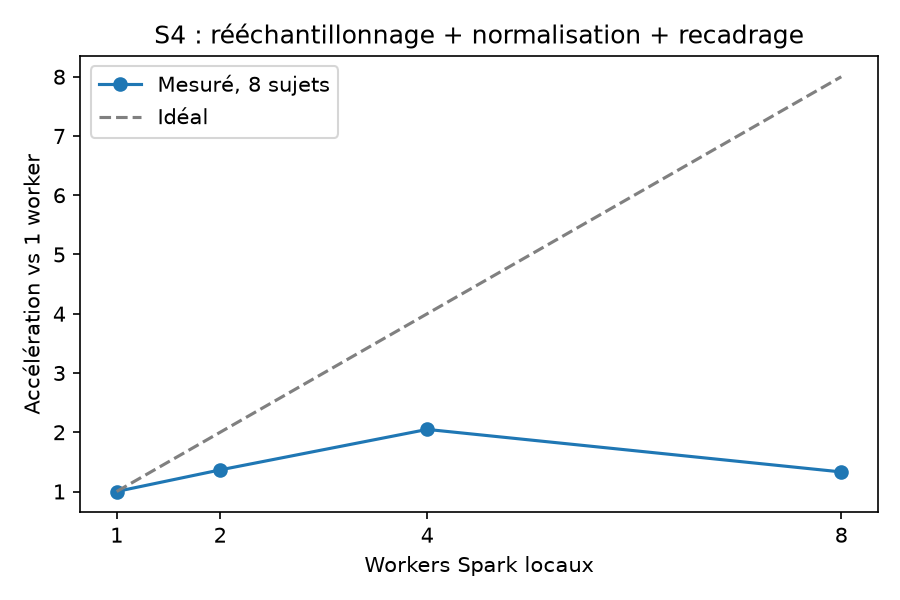
\includegraphics[width=0.6\linewidth]{preprocessing/reports/benchmark_speedup.png}
  \caption{Accélération du prétraitement S4 selon le nombre de workers Spark locaux (8 sujets, un essai).}
  \label{fig:yosra-benchmark}
\end{figure}

\section{Statistiques et empreinte du centre}
\label{sec:yosra-s5-s6}

Les rapports S5 comparent les distributions avant/après prétraitement et mesurent les distances Wasserstein et MMD entre centres et référence.
Le z-score contraint moyenne et variance par scan ; les différences restantes portent donc surtout sur la forme des distributions.
Les échelles avant/après ne sont pas identiques : leur comparaison normalisée reste descriptive.

Le test S6 prédit le centre depuis des histogrammes ou statistiques, avec cinq plis stratifiés, exactitude équilibrée et contrôle à labels mélangés.
Comparer des histogrammes de granularité proche et les mêmes patients permet de mieux isoler l'effet du prétraitement.
Une empreinte reconnaissable n'implique pas à elle seule une baisse du Dice.

Valeurs et figures : \nolinkurl{analysis/reports/post_stats_summary.json}, \nolinkurl{analysis/reports/site_fingerprint_s6.csv}, figures~\ref{fig:yosra-s5-avant-apres}, \ref{fig:yosra-s5-distances} et~\ref{fig:yosra-s6}.
Les versions historiques sur 1\,402 cas ne doivent pas être confondues avec la relance sur 1\,415.
Les versions historiques sur 1\,402 cas sont conservées dans l'historique Git du dépôt
(commit \texttt{5a86471}, fichier \texttt{analysis/reports/post\_stats\_summary.json}).

La relance du 11 novembre couvre 1\,415 sujets dans 54 centres.
La distance relative médiane passe de 0,1315 avant à 0,0376 après, sur la même cohorte disponible.
La corrélation entre Wasserstein et MMD vaut 0,842 pour les centres d'au moins cinq scans.
La médiane de Wasserstein vaut 0,0376 pour ID et 0,0900 pour OOD ; cet écart reste affecté par la sélection initiale des centres (\nolinkurl{analysis/reports/post_stats_summary.json}).
Le test S6 retient 1\,140 scans de 25 centres.
Avec les histogrammes 32 classes avant / 30 classes après et le meilleur des deux classifieurs, l'exactitude équilibrée vaut 69,7~\% puis 48,9~\%.
Le contrôle mélangé vaut 4,0~\%, proche du hasard à 4~\% (\nolinkurl{analysis/reports/site_fingerprint_s6.csv}, \nolinkurl{analysis/reports/site_fingerprint_s6_summary.json}).
Ces chiffres ne mesurent pas la performance de segmentation.

\begin{figure}[p]
  \centering
  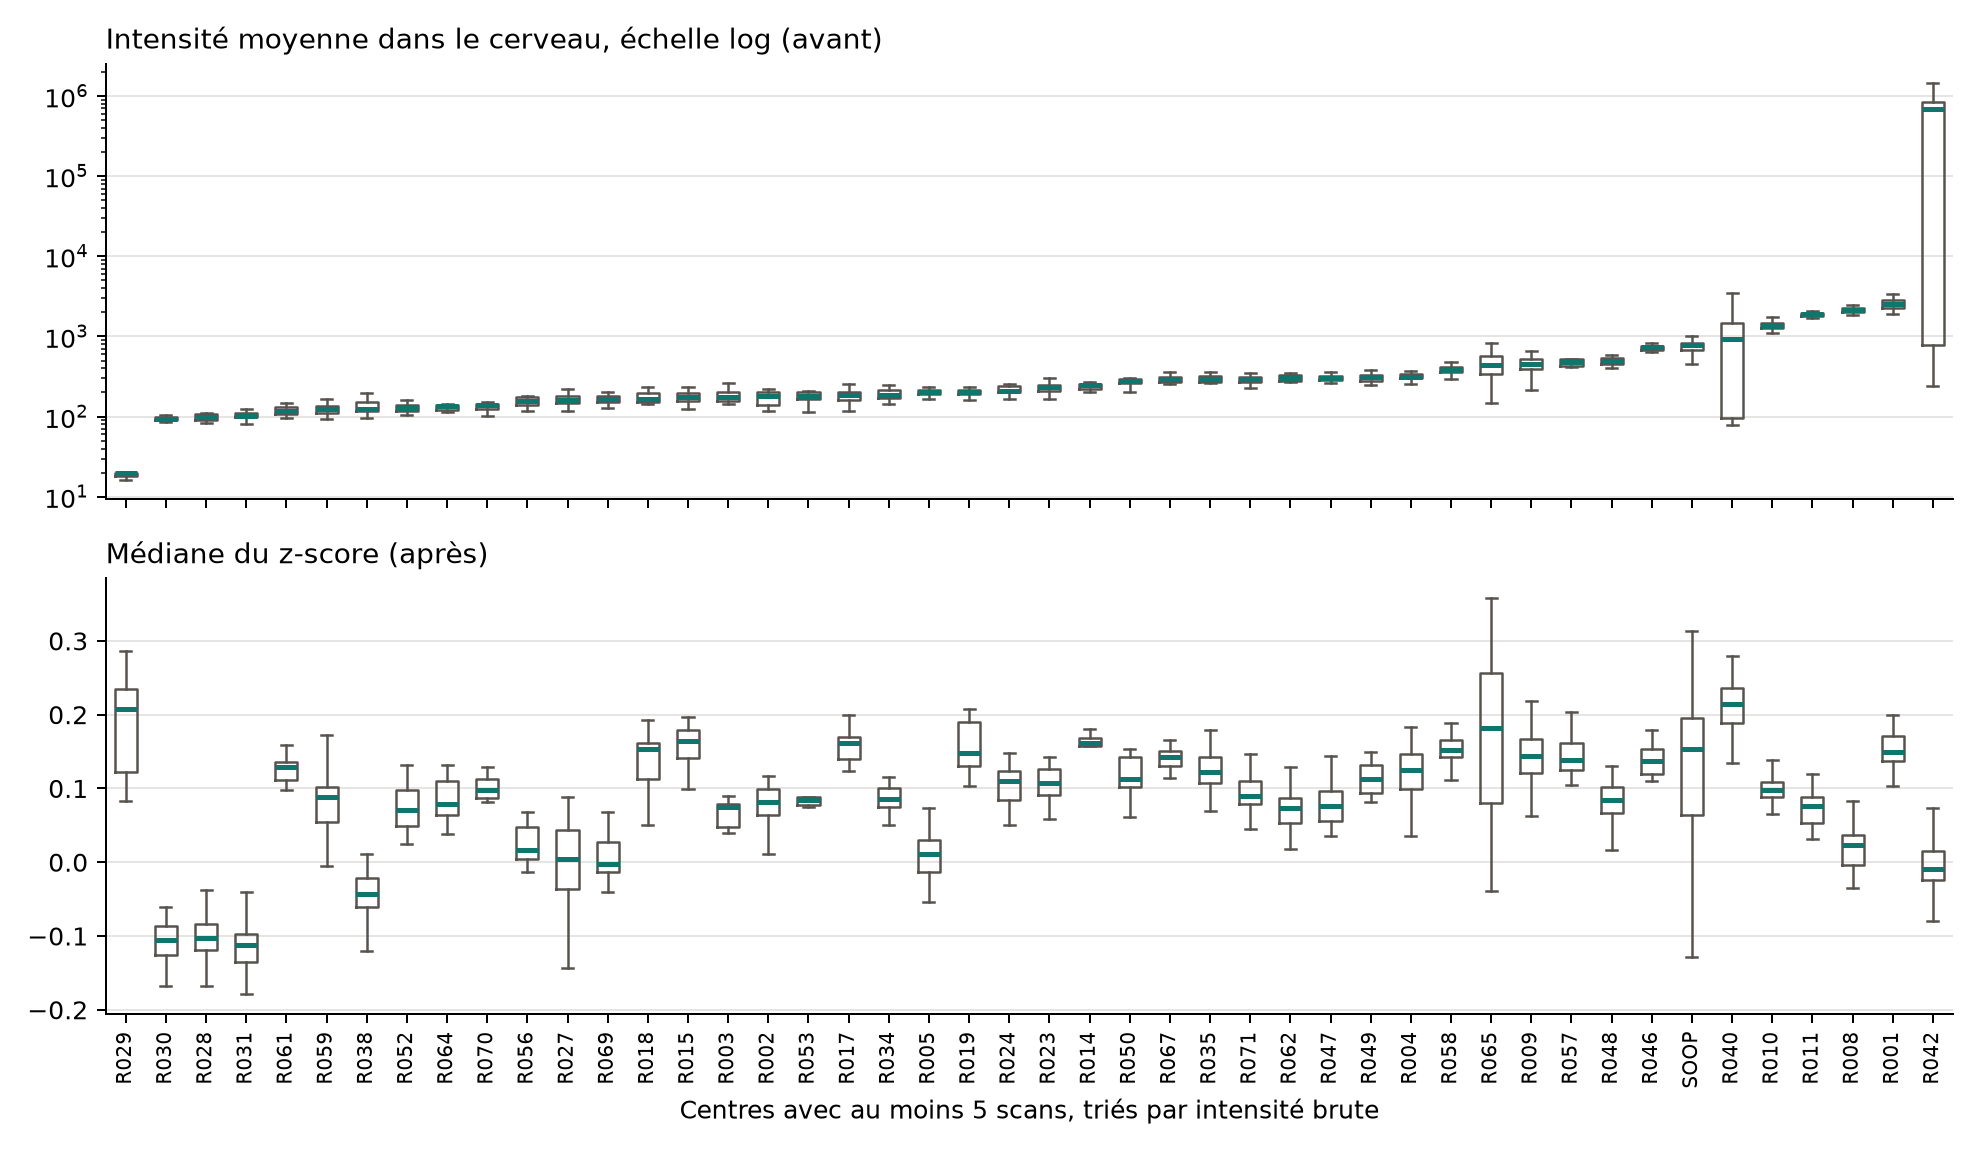
\includegraphics[angle=90,height=0.9\textheight]{figures/s5_avant_apres_par_centre.png}
  \caption{Intensité moyenne dans le cerveau avant prétraitement (échelle log) et médiane du z-score après, par centre (centres d'au moins 5 scans).}
  \label{fig:yosra-s5-avant-apres}
\end{figure}

\begin{figure}[htbp]
  \centering
  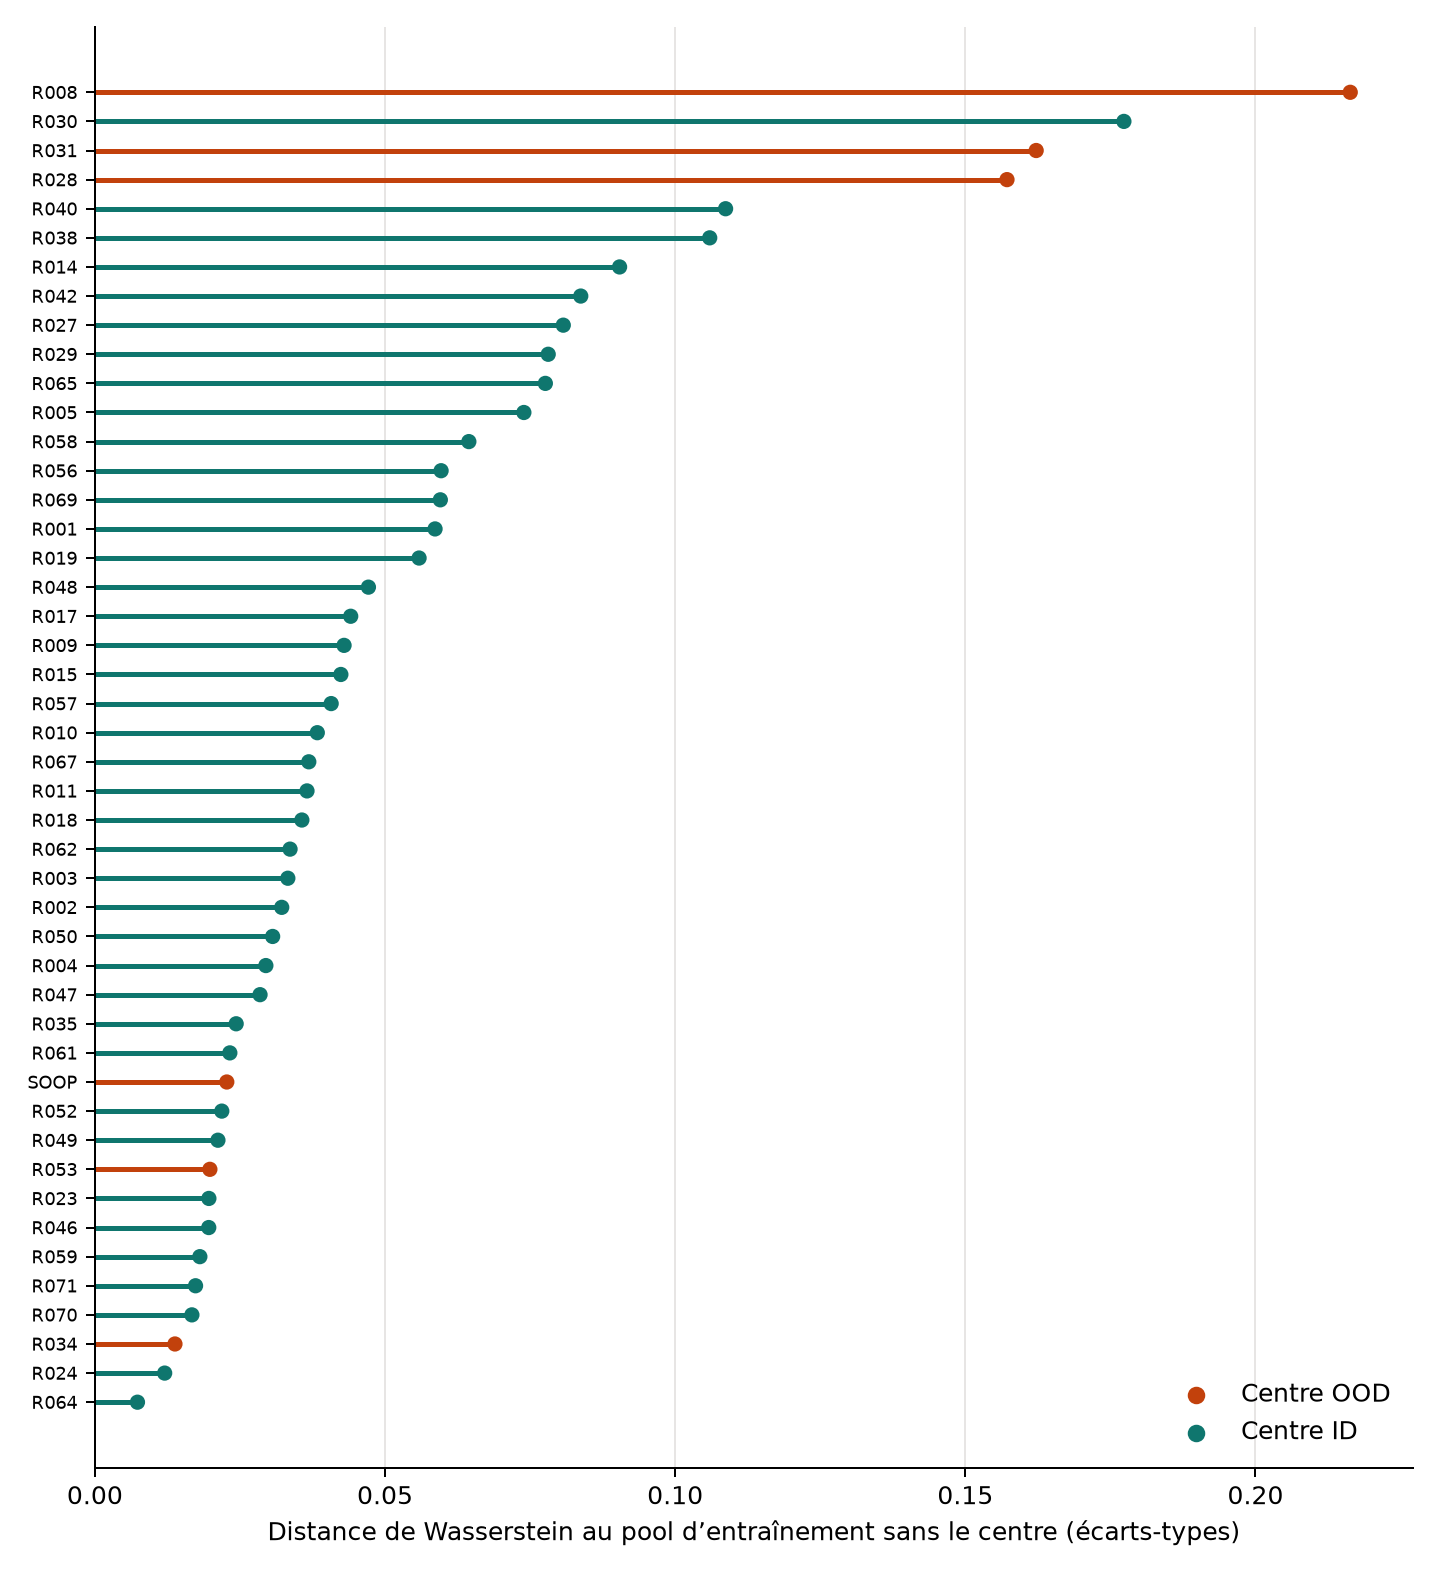
\includegraphics[width=0.85\linewidth]{figures/s5_distances_centres.png}
  \caption{Distance de Wasserstein de chaque centre au pool d'entraînement sans ce centre ; centres OOD en orange.}
  \label{fig:yosra-s5-distances}
\end{figure}

\begin{figure}[htbp]
  \centering
  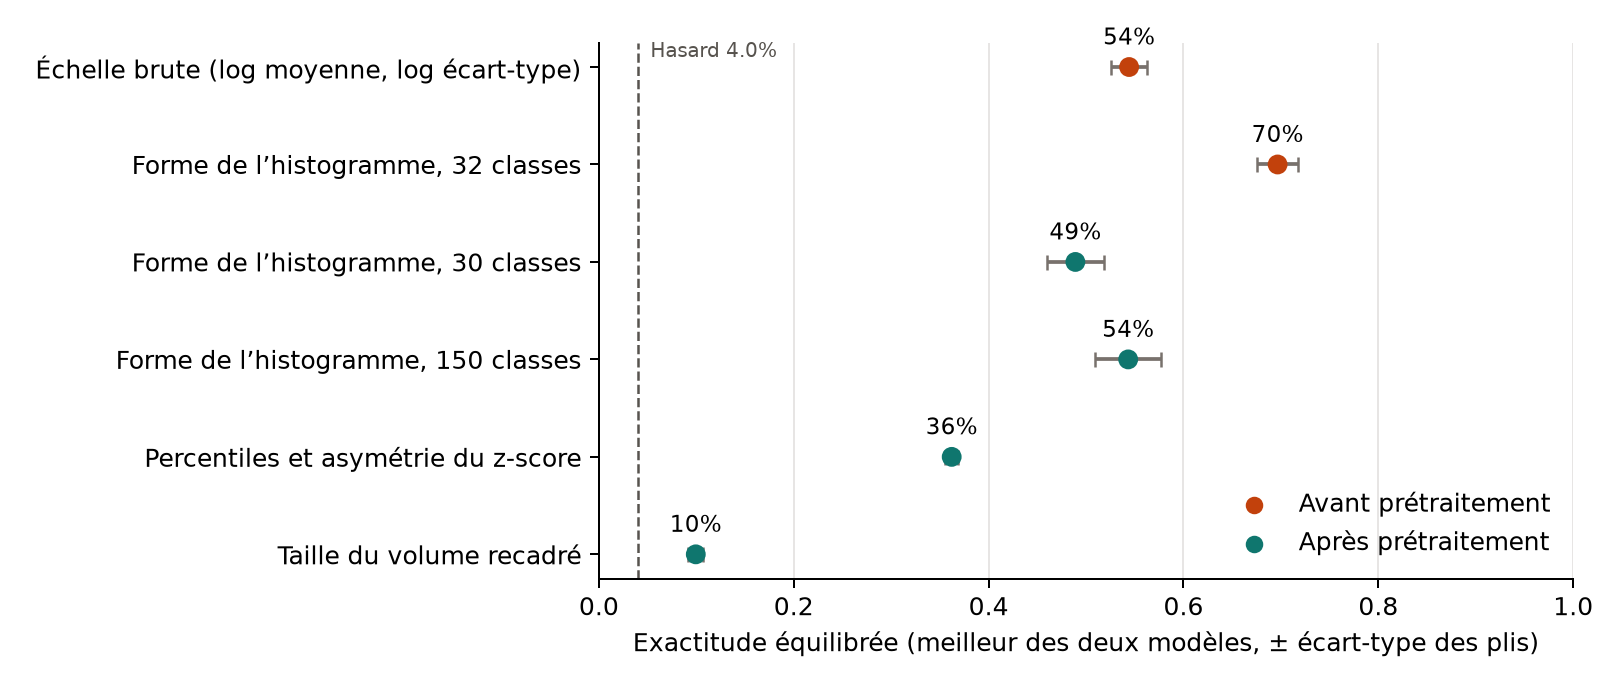
\includegraphics[width=\linewidth]{figures/s6_empreinte_centre.png}
  \caption{Empreinte du centre (S6) : exactitude équilibrée de la prédiction du centre selon la représentation, avant et après prétraitement (hasard : 4~\%).}
  \label{fig:yosra-s6}
\end{figure}

\section{Prédiction d'échec et effet du temps : protocole C1 préparé}
\label{sec:yosra-s7-s8}

S7 met en relation la distance au train du pli et l'erreur $1 - \mathrm{Dice}$ par centre.
Une validation leave-one-center-out produit des prédictions hors calibration.
La régression et le seuil d'alerte sont ajustés uniquement sur les autres centres de validation.
La différence de Dice par rapport au test ID est rapportée séparément.
Sans les résultats C3 de C1, ni corrélation empirique ni performance d'alerte ne peuvent être annoncées.

S8 compare les associations du centre et du délai post-AVC par modèles linéaires emboîtés sur les mêmes cas complets.
Le délai est transformé par $\log(1 + \textrm{jours})$.
Le test de permutation préserve le centre.
Les délais manquants, la sélection des cas et les confusions possibles limitent l'interprétation.
Le protocole n'établit pas une relation causale.

\section{Caractéristiques du réseau (C6 v2)}
\label{sec:yosra-c6}

La version C6 v2 mesure le décalage dans l'espace appris par le réseau plutôt que sur les
intensités. Le modèle C8 (U-Net 3D, augmentation d'intensité, pli 0) est gelé et utilisé en
mode évaluation, sans gradient et sans masque lésionnel. Pour chaque sujet, la sortie du
bottleneck, la couche que lit le classifieur de centre de DANN, est moyennée dans l'espace :
on obtient un vecteur de 320 valeurs par scan.
L'entrée est le volume C1 complet, complété par des zéros jusqu'à un multiple de 16. Le réseau
a été entraîné sur des patchs $96^3$ : sur le volume entier, les normalisations d'instance
portent sur une autre étendue. La même règle est appliquée à tous les scans, ce qui garde la
comparaison entre centres cohérente.

La comparaison d'empreinte baseline / augmentation / DANN demande les checkpoints baseline et
DANN du même protocole ; elle reste à faire.

\section{Démonstration et limites}
\label{sec:yosra-demo}

L'application Gradio affiche les coupes d'une IRM et un masque, calcule le volume lésionnel en mL et accepte une carte d'incertitude.
Un adaptateur permet de brancher le modèle final.
NiiVue fournit une vue 3D locale sur la route \texttt{/viewer/} du même serveur.
ANTsPy peut recaler un template MNI et transférer un atlas de labels ; une inspection visuelle demeure nécessaire avant de nommer les régions.

L'alerte individuelle d'intensité utilise un quantile de validation distinct du seuil par centre.
Elle n'est ni une garantie de performance ni une décision clinique.
En l'absence d'une entrée requise, l'application indique ce qui manque au lieu de créer un résultat.
Le support animé de secours est synthétique et explicitement étiqueté.

\subsection{Interface web du projet}
\label{sec:yosra-frontend}

Une application web (\texttt{frontend/}) présente l'ensemble du projet en dix pages :
vue d'ensemble, avancement du pipeline, contrôle qualité, prétraitement Spark, décalage entre
centres, modèles et Dice, adaptation de domaine, démonstration IRM avec vue 3D, conclusions
et galerie des figures. Le serveur FastAPI lit uniquement les rapports versionnés du dépôt
(\texttt{analysis/reports}, \texttt{preprocessing/reports}, \texttt{baselines/outputs},
\texttt{adaptation/outputs}, \texttt{integration/reports}) : aucun chiffre n'est simulé, et une
expérience absente est signalée comme telle. Chaque page et chaque carte indiquent qui a
produit le résultat. L'interface fonctionne sans étape de construction ni ressource externe ;
seules les figures des dossiers de résultats sont servies, jamais les données IRM. Sept tests
couvrent l'API (\texttt{frontend/tests/test\_server.py}).

\subsection{Branchement du modèle C8}
\label{sec:yosra-c8}

La démonstration (\texttt{demo/app.py}) et l'interface web appellent la fonction désignée par
la variable \texttt{AVC\_PREDICT\_ADAPTER}, au format \texttt{module:fonction}. L'adaptateur de
l'équipe, \texttt{adaptation.demo\_adapter:predict}, applique le prétraitement S4 puis le modèle
retenu (augmentation d'intensité, pli 0) et enregistre le masque en NIfTI \texttt{uint8} dans la
grille de l'IRM reçue. Il demande PyTorch et MONAI, absents de l'environnement de la
démonstration. Le pont \texttt{demo/c8\_bridge.py} lance donc cet adaptateur dans
l'environnement du modèle, dans un processus séparé, et récupère le masque ; la démonstration
utilise \texttt{AVC\_PREDICT\_ADAPTER=c8\_bridge:predict}. Le checkpoint est lu dans
\texttt{data/modeles/unet3d\_intensity\_pli0\_best.pt} (SHA-256 \texttt{ee6b93af\ldots abb6}),
hors du dépôt.

Sur le sujet OOD R034\_sub-r034s003\_ses-1, le rapport de la démonstration donne un volume
lésionnel de 27,058~mL (27\,058 voxels de 1~mm$^3$). Cette valeur concorde avec le volume
prédit lors de l'évaluation du modèle : 27,054~mL dans le fichier \texttt{resultats\_ood\_test.csv}
de la run intensité, conservé hors du dépôt. Sur le sujet OOD R031\_sub-r031s006\_ses-1, envoyé
sans masque à l'interface web, le modèle prédit 33,8~mL pour 27,7~mL annotés, soit un Dice de
0,745, en environ 35~s sur processeur. Ces deux cas vérifient le branchement ; ils ne constituent
pas une évaluation. Le modèle ne produit pas de carte d'incertitude. Cinq tests couvrent les
erreurs du pont (\texttt{tests/test\_c8\_bridge.py}).

\section{Discussion et travaux à terminer}
\label{sec:yosra-discussion}

Les principales limites actuelles sont la quarantaine QC à relire collectivement, le faible nombre de centres pour calibrer un prédicteur d'échec, la dépendance des distances aux effectifs, les métadonnées manquantes et l'absence locale des checkpoints et des Dice correspondant à C1 v2.
Les résultats RQ3 du pli 0 et le checkpoint C8 sont désormais disponibles (chapitre RQ3,
conclusion). Les analyses S7 et S8 sur C1 v2 attendent encore les Dice par sujet, y compris
sur la validation, qui sert à calibrer le seuil d'alerte sans consulter le test. L'empreinte
avant/après DANN attend les checkpoints baseline et DANN. La vidéo de vraie inférence et la
relecture collective restent à faire.
Une analyse S8 historique distincte est disponible plus bas (section~\ref{sec:yosra-s8-historique}).
Les références bibliographiques du document de projet doivent être vérifiées dans leurs publications originales avant d'être reprises dans la version remise.

\section{Compléments vérifiés de la livraison v2}
\label{sec:yosra-livraison}

L'export nnU-Net contient 916 images et labels d'entraînement, 499 images de test (231 ID, 268 OOD) et cinq plis (\nolinkurl{preprocessing/reports/export_v2.json}).
Le contrôle officiel nnU-Net reste à lancer dans l'environnement d'entraînement de Fayfa.
Les autres appartenances de v1 sont conservées.

L'analyse descriptive S8 trouve 1\,073 délais utilisables et 342 manquants ou invalides ; le délai médian est de 365 jours.
Huit centres n'ont aucun délai utilisable.
L'association centre / log-délai (eta carré 0,7475) souligne la nécessité de tenir compte du centre ; elle ne mesure pas l'effet du délai sur le Dice.
Voir \nolinkurl{analysis/reports/s8_metadata/} (\nolinkurl{summary.json}).

Le seuil individuel d'atypie du pli~0 vaut 0,114885 : référence de 733 scans du train, quantile 95~\% sur 183 scans de validation.
Aucun test ID/OOD n'a servi à ce réglage.
Le seuil est enregistré dans \texttt{data/demo/reference\_ood.json} (pli 0, quantile 0,95,
733 scans d'entraînement, 183 de validation), hors du dépôt comme l'ensemble de \texttt{data/}.

Chrome a chargé l'application, produit le rapport synthétique de 2,091~mL, puis affiché les coupes et le rendu 3D NiiVue sans erreur JavaScript (\nolinkurl{docs/pipeline/demo_verification/browser_report.json}).
L'image Docker a été construite et ses routes ainsi que le calcul du rapport ont été testés (\nolinkurl{docs/pipeline/verification.json}).
La vidéo de secours MP4 utilise ces captures réelles d'interface sur un phantom explicitement synthétique ; elle ne montre pas une inférence du réseau.

L'atlas Harvard-Oxford et le template compatible MNI152NLin6Asym ont été récupérés avec leurs sources et empreintes dans \nolinkurl{data/demo/atlas/provenance.json} (hors du dépôt ; copie versionnée : \nolinkurl{docs/pipeline/demo_verification/atlas_provenance.json}).
Les labels corticaux sont prioritaires, puis les labels sous-corticaux décalés de 100 ; les zones non couvertes gardent la valeur zéro.
Le recalage natif exige une relecture anatomique.
Sources : Nilearn Harvard-Oxford\footnote{\url{https://nilearn.github.io/stable/modules/generated/nilearn.datasets.fetch_atlas_harvard_oxford.html}} et TemplateFlow MNI152NLin6Asym\footnote{\url{https://github.com/templateflow/tpl-MNI152NLin6Asym}}.

Le recalage SyN sur l'exemple réel a été exécuté.
Atlas et IRM ont la même grille, les labels restent entiers et 97,75~\% des voxels atlas non nuls se trouvent dans le support d'intensité de l'image (\nolinkurl{docs/pipeline/verification.json}).
La planche locale \nolinkurl{data/demo/registration/qc_overlay.png} (hors du dépôt) a été examinée dans trois plans ; cela ne remplace pas une relecture anatomique experte.
Le rapport régional utilise le masque de référence fourni, sans inférence de réseau.

\section{S8 : résultat exploratoire sur les baselines récupérées}
\label{sec:yosra-s8-historique}

Le 12 novembre, les scores historiques de \texttt{cnn\_pretrained\_freeze-none} ont été rattachés à leur propre partition (903 train, 226 ID validation, 287 OOD), sans les reclasser dans C1 v2.
L'analyse utilise 167 cas ID complets de 31 centres et 257 cas OOD de 12 centres.
En ID, 58 délais manquent ou sont invalides et un Dice est absent ; en OOD, 30 délais manquent ou sont invalides.
Le Dice absent du cas à masque vide n'est pas remplacé par un score supposé.

Après ajustement sur le centre, l'ajout de $\log(1 + \textrm{délai})$ augmente le R$^2$ de 0,000046 en ID ($p$ exploratoire $= 0{,}911$) et de 0,03808 en OOD ($p = 0{,}001$ ; 999 permutations intra-centre pour chaque groupe).
Après ajout de $\log(1 + \textrm{volume lésionnel})$, ces gains sont respectivement 0,000711 et 0,000217 (\nolinkurl{analysis/reports/s8_historical/summary.json}).
L'association OOD dépend donc fortement des variables prises en compte ; elle ne permet pas d'attribuer un effet causal au temps.
Le volume est une analyse de sensibilité, pas un ajustement causal validé.
La figure~\ref{fig:yosra-s8} montre les cas utilisés.

\begin{figure}[htbp]
  \centering
  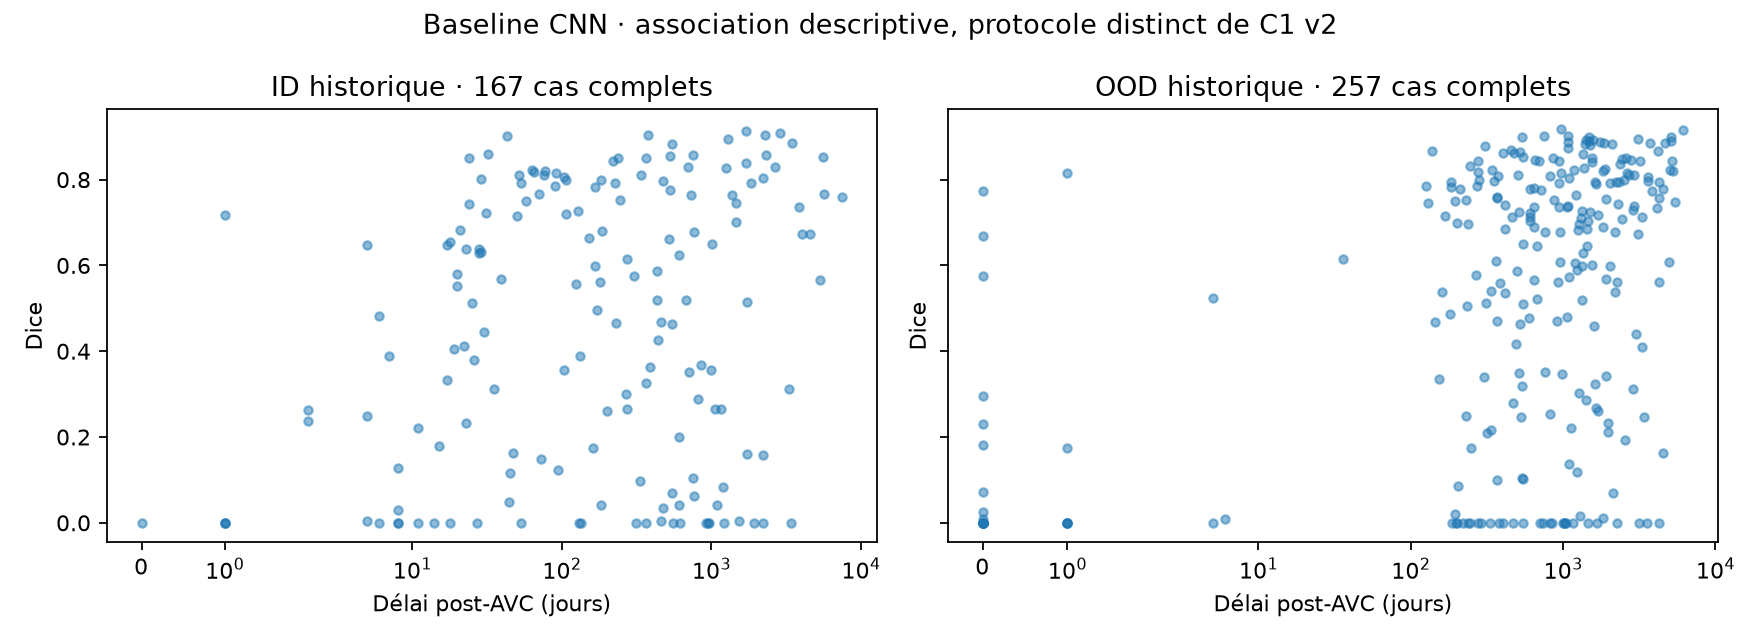
\includegraphics[width=\linewidth]{analysis/reports/s8_historical/time_dice.png}
  \caption{Dice de la baseline CNN historique selon le délai post-AVC, cas complets ID (167) et OOD (257) ; protocole distinct de C1 v2.}
  \label{fig:yosra-s8}
\end{figure}

Ces deux tests sont exploratoires, sans correction de multiplicité.
L'ID a participé au choix historique du modèle et n'est pas un test indépendant.
La partition et le prétraitement diffèrent de C1 v2.
Les résultats des autres baselines sont résumés séparément sur leurs effectifs disponibles, sans comparaison appariée implicite.

Livrables reproductibles : \nolinkurl{analysis/historical_baselines.py}, \nolinkurl{analysis/reports/s8_historical/summary.json}, \nolinkurl{README.md}, \nolinkurl{model_summary.csv}, \nolinkurl{missing_by_center.csv} et \nolinkurl{time_dice.png}.
Les empreintes des fichiers sources sont conservées.

\section{S6 : complément sur l'incertitude}
\label{sec:yosra-s6-incertitude}

Une évaluation complémentaire utilise 912 sujets d'entraînement et 228 sujets réservés, stratifiés parmi les mêmes 25 centres.
Deux classifieurs fixés, régression logistique et forêt aléatoire, sont évalués sur les mêmes sujets.
Les sujets réservés sont ensuite rééchantillonnés 10\,000 fois à l'intérieur de chaque centre, avec les mêmes indices pour toutes les représentations ; l'exactitude équilibrée donne le même poids aux centres.

Pour la forêt aléatoire, le score avant traitement (32 classes) est de 70,1~\%, avec un intervalle percentile conditionnel à 95~\% de [64,6 ; 75,5]~\%.
Après traitement (30 classes), il est de 51,1~\% [45,3 ; 57,0]~\%.
La différence appariée après moins avant est de $-19{,}0$ points [$-25{,}5$ ; $-12{,}6$].
Pour la régression logistique, elle est de $-21{,}5$ points [$-27{,}4$ ; $-15{,}5$] (\nolinkurl{analysis/reports/s6_uncertainty/intervals.csv}, \nolinkurl{analysis/reports/s6_uncertainty/paired_differences.csv}).
La variante après traitement à 150 classes est aussi rapportée pour montrer la sensibilité à la représentation, sans sélectionner uniquement le meilleur score.
La figure~\ref{fig:yosra-s6-incertitude} présente ces intervalles.

\begin{figure}[htbp]
  \centering
  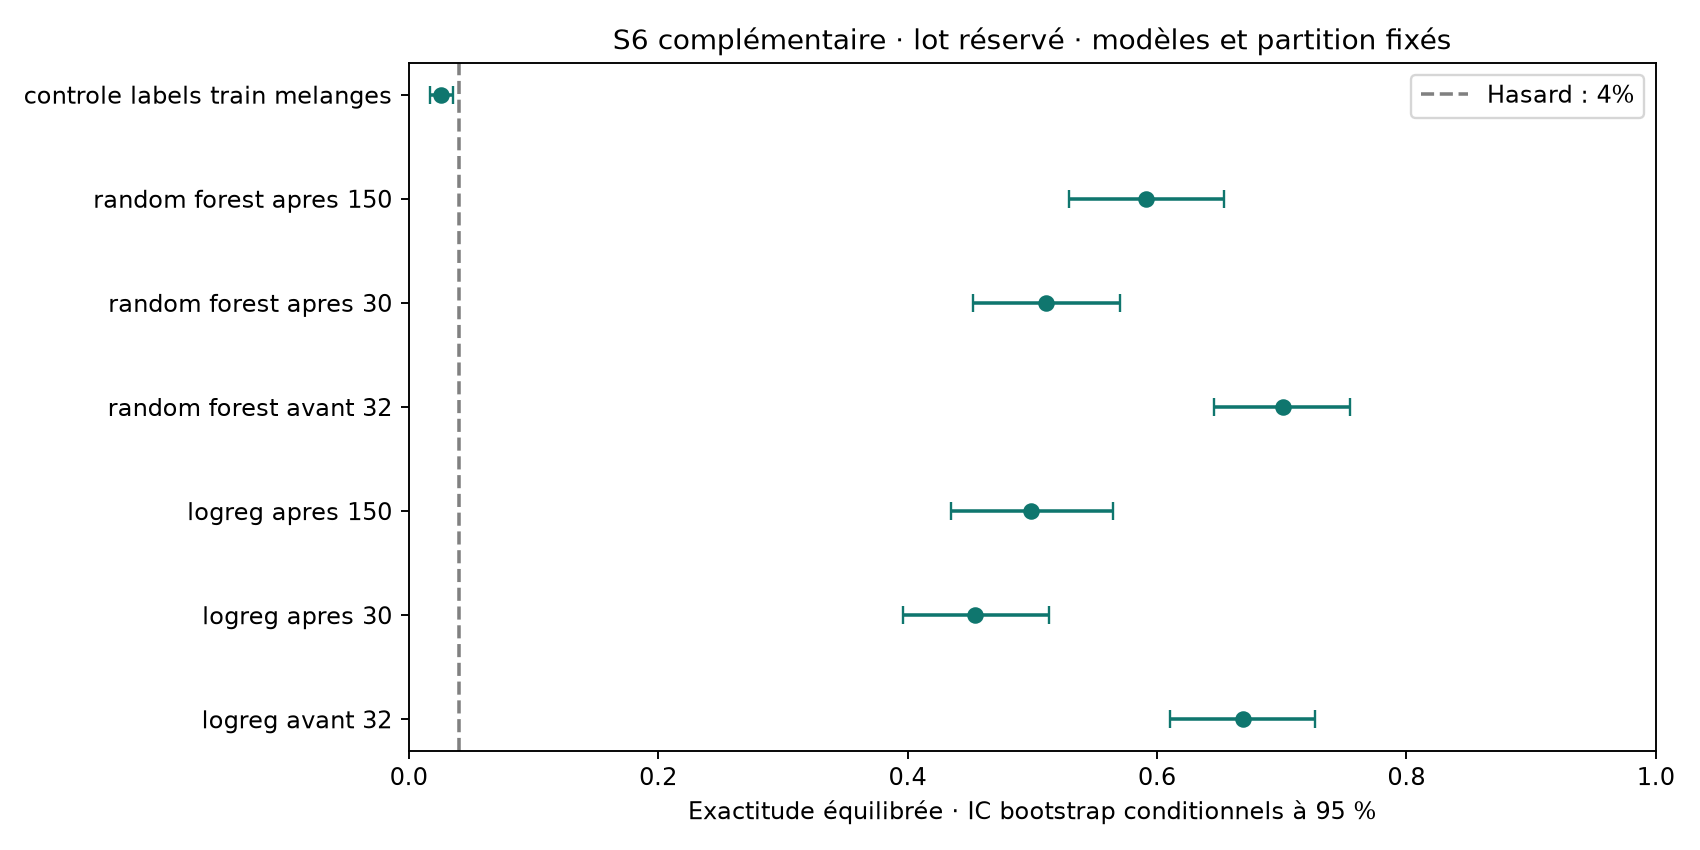
\includegraphics[width=\linewidth]{analysis/reports/s6_uncertainty/confidence_intervals.png}
  \caption{Exactitude équilibrée de la reconnaissance du centre sur le lot réservé, avec IC bootstrap conditionnels à 95~\% (modèles et partition fixés).}
  \label{fig:yosra-s6-incertitude}
\end{figure}

Ces intervalles conditionnent sur les modèles et la partition fixés : ils n'incluent pas la variabilité d'un nouvel entraînement.
La cohorte avait déjà été explorée en S6, et la granularité avant/après reste différente.
Il s'agit d'un complément exploratoire, pas d'une validation externe ni d'un effet causal isolé du prétraitement.
Les centres sont présents dans le train et le test : l'expérience mesure leur reconnaissance, pas la segmentation dans un centre inconnu.
Les moyennes des cinq plis précédentes restent inchangées et ne doivent pas être confondues avec ces nouveaux scores.

Livrables : \nolinkurl{analysis/reports/s6_uncertainty/README.md}, \nolinkurl{intervals.csv}, \nolinkurl{paired_differences.csv}, \nolinkurl{summary.json} et \nolinkurl{confidence_intervals.png}.
Les prédictions individuelles restent dans \nolinkurl{data/analysis/s6_uncertainty/} (hors du dépôt).

\section{Synthèse du contrôle qualité par centre}
\label{sec:yosra-qc}

La synthèse couvre les 1\,453 sujets inventoriés dans 55 centres.
Elle retrouve 1\,415 sujets retenus dans 54 centres, 38 exclus et aucune erreur active.
Les exclusions correspondent aux 37 cas R032 pour espacement non fiable et au cas R065 mis en quarantaine pour annotation hors du support et du recadrage.
Cette synthèse n'ajoute aucune exclusion et ne remplace pas la relecture collective des décisions.

Parmi les 1\,415 sujets retenus, cinq masques sont vides et conservés comme cas négatifs ; 1\,410 sont non vides et aucun statut de masque n'est inconnu.
Le délai post-AVC est disponible pour 1\,073 sujets ; 342 délais sont manquants ou invalides (24,2~\%).
Huit centres retenus n'ont aucun délai utilisable.
Le drapeau CHRONICITY est présent pour 296 sujets et non renseigné pour 1\,119 ; cette absence ne permet pas de déduire un stade clinique.
Deux sujets SOOP portent l'avertissement de fichier de métadonnées vide : cet avertissement de fichier ne recouvre pas toutes les valeurs de délai absentes.

Les effectifs d'exclusion utilisent tout l'inventaire ; les pourcentages de métadonnées utilisent seulement les sujets retenus de chaque centre.
Pour R032, sans sujet retenu, les taux sont non définis plutôt que nuls.
Les colonnes inconnues ne sont pas assimilées à des masques non vides.
Le tableau détaillé, la figure, les motifs d'exclusion et les avertissements sont disponibles dans \nolinkurl{analysis/reports/qc_by_center/} (\nolinkurl{summary.json}, \nolinkurl{qc_by_center.csv}, \nolinkurl{exclusion_reasons.csv}, \nolinkurl{metadata_warnings.csv}).
% La figure qc_by_center.png (55 centres sur trois panneaux) n'est pas insérée : à la largeur de la page, son texte
% ferait environ 3 pt. Elle reste disponible dans analysis/reports/qc_by_center/.
\section{Vérification de l'intégration}
\label{sec:yosra-verification}

Après la fusion des contributions de l'équipe dans \texttt{main}, 310 tests réussissent :
50 pour le pipeline et les analyses, 7 pour l'interface web, 224 pour la généralisation et
l'adaptation (dont des patchs C1 réels) et 29 pour la calibration. Quatorze tests
d'entraînement (\texttt{adaptation/tests/test\_train.py}, \texttt{test\_continual.py}) échouent
sur le Mac de vérification : \texttt{torch.amp.GradScaler} n'existe pas dans torch 2.2.2,
dernière version disponible pour macOS Intel. L'entraînement est exécuté sur Kaggle ;
l'inférence du checkpoint C8 est vérifiée localement
(\texttt{integration/reports/verification.json}).

\setlength{\emergencystretch}{0pt}
. Version LaTeX de docs/pipeline/RAPPORT.md (commit 4540d85) :
% plan, contenu et formulations conservés ; chemins des fichiers sources ajoutés pour chaque chiffre.
% Paquets attendus dans le préambule : babel (french), graphicx, booktabs, makecell, hyperref, float.
% Réglages à mettre dans le préambule du rapport final :
%   \addto\captionsfrench{\def\tablename{Tableau}}   % « Tableau » au lieu de « Table »
%   \hypersetup{hidelinks}                             % liens sans cadre rouge
% Les chemins des figures sont relatifs à la racine du dépôt.
% Statut d'origine (RAPPORT.md) : brouillon scientifique fondé sur les résultats locaux disponibles ; les valeurs
% finales doivent être prises dans les JSON/CSV générés après le dernier QC ; les expériences sans prédictions ou
% checkpoints ne sont pas présentées comme réalisées.

% Chemins de fichiers longs : coupures de ligne aussi permises après « _ » et « - » dans \nolinkurl et \url.
\makeatletter
\g@addto@macro\UrlBreaks{\do\_\do\-}
\makeatother
% Étirement d'urgence limité à ce chapitre (lignes chargées de chemins), remis à zéro à la fin.
\setlength{\emergencystretch}{3em}

\chapter{Données, décalage de domaine et démonstration}
\label{chap:yosra}

\section{Introduction et questions de recherche}
\label{sec:yosra-introduction}

Ce projet étudie la segmentation des lésions d'AVC sur des IRM T1 acquises dans plusieurs centres.
Les différences de scanner, protocole et résolution peuvent modifier la distribution des images.
Notre objectif est de mesurer ce décalage, d'évaluer la généralisation des modèles sur des centres absents de l'entraînement, puis d'étudier la possibilité d'anticiper et de réduire leur perte de performance.

Trois questions structurent le projet : quel est l'écart entre test ID et test OOD ?
Les architectures Transformer améliorent-elles la généralisation par rapport à nnU-Net ?
Quelles techniques de généralisation ou d'adaptation réduisent cet écart ?
La contribution de Yosra fournit le pipeline de données, les partitions communes, les mesures du décalage, les analyses explicatives et l'interface de démonstration.
Les comparaisons de segmentation et l'adaptation continue sont produites par Fayfa et Anas.

\section{Données et contrôle qualité}
\label{sec:yosra-donnees}

L'inventaire local contient 1\,453 paires IRM/masque dans 55 centres.
Le centre R032, soit 37 cas, est exclu provisoirement pour espacement incohérent.
Les métadonnées vides sont signalées sans supprimer une paire utilisable.
Les masques vides sont conservés comme cas négatifs.
Le délai post-AVC reste numérique ; \texttt{CHRONICITY}, codé 1/vide, n'est pas interprété comme une catégorie aigu/subaigu/chronique
(\nolinkurl{analysis/reports/qc_by_center/summary.json}, \nolinkurl{analysis/reports/qc_by_center/exclusion_reasons.csv}).

La livraison v2 contient 1\,415 volumes prétraités, relus et exportés.
Elle exclut les 37 cas R032 et met un cas supplémentaire en quarantaine technique.
Le split v1 est archivé ; v2 retire uniquement ce cas, sans déplacer les autres sujets ni les centres.
La relecture collective de cette quarantaine reste nécessaire ; les annotations brutes sont intactes
(\nolinkurl{preprocessing/reports/release_v2.json}, \nolinkurl{preprocessing/qc_exclusions.json}).

\section{Pipeline Spark}
\label{sec:yosra-pipeline}

Chaque sujet constitue une unité de travail.
Le pipeline réoriente les images en RAS, rééchantillonne à 1~mm isotrope (linéaire pour l'image, plus proche voisin pour les masques), normalise les intensités dans le support cérébral et recadre avec une marge de cinq voxels.
Le support est défini par les intensités supérieures à la valeur de fond estimée ; cette précaution traite notamment le centre R029 dont le fond n'est pas nul.
Cette heuristique reste une limite et doit être examinée sur les cas atypiques.

Le z-score est stocké en \texttt{int16} avec un pas de 0,001.
L'erreur d'arrondi est au plus 0,0005 unité de z-score.
Le validateur utilise cette borne, avec une petite marge numérique, pour la moyenne et l'écart-type ; le fond doit rester exactement nul.
Une signature des entrées et paramètres permet la reprise et chaque paire est accompagnée d'un QC (\nolinkurl{preprocessing/week4.py}).

La boîte de recadrage est déterminée par l'image seule.
Le code existant tolère la suppression de labels hors boîte jusqu'à 1~\% du volume lésionnel.
Ce choix n'est pas une correction clinique des annotations : il doit être documenté et validé.
Le dernier cas dépasse cette tolérance (1,76~\% : 77 voxels sur 4\,376, \nolinkurl{preprocessing/qc_exclusions.json}) et est mis en quarantaine dans v2.
L'option N4 a été ajoutée pour une expérience distincte ; elle n'a pas été appliquée au jeu de référence et aucun bénéfice n'en est revendiqué.

\section{Partitions et absence de fuite}
\label{sec:yosra-partitions}

Le fichier commun \nolinkurl{splits.json} version 2 fixe 916 cas d'entraînement/validation, 231 cas ID et 268 cas OOD (\nolinkurl{preprocessing/reports/release_v2.json}).
Six centres OOD sont intégralement retirés : R008, R028, R031, R034, R053 et SOOP.
Les cinq plis séparent les centres d'entraînement et de validation.
Le test ID de chaque pli est limité aux centres présents dans son entraînement.
Le découpage compte 231 sujets ID au total ; pour le pli~0, le test ID n'en garde que 185, car les 46 autres appartiennent aux centres de validation de ce pli, absents de son entraînement (\nolinkurl{splits.json}, \texttt{folds[0].id\_test}).

La sélection des centres OOD varie taille et distance d'intensité.
Comme la distance participe à cette sélection, un écart de distance ID/OOD n'est pas une découverte indépendante.
Les mesures prédictives doivent utiliser la référence d'entraînement du modèle considéré, pas le pool global.
Aucun hyperparamètre d'alerte ne doit être choisi sur le test OOD.

\section{Benchmark}
\label{sec:yosra-benchmark}

Le pilote existant porte sur huit petits volumes et un essai par configuration.
Les temps de calcul sont 56,59~s, 41,46~s, 27,63~s et 42,54~s pour 1, 2, 4 et 8 workers.
L'accélération maximale mesurée est $\times$2,05 avec quatre workers (\nolinkurl{preprocessing/reports/benchmark_summary.csv}, \nolinkurl{preprocessing/reports/benchmark_scope.json}).
La dégradation à huit workers est compatible avec des coûts de concurrence et de ressources ; ce pilote ne permet pas d'en isoler la cause.
Les workers ne constituent pas des cœurs physiques réservés.
Le démarrage Spark n'entre pas dans \texttt{compute\_seconds}.
Les courbes ne sont pas extrapolées au dataset entier.
La figure~\ref{fig:yosra-benchmark} montre l'accélération mesurée.

\begin{figure}[htbp]
  \centering
  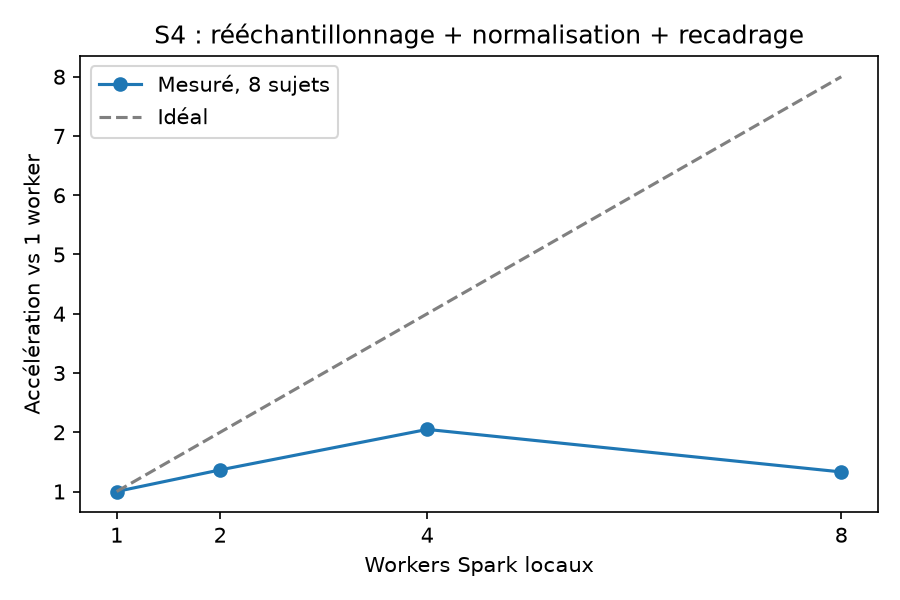
\includegraphics[width=0.6\linewidth]{preprocessing/reports/benchmark_speedup.png}
  \caption{Accélération du prétraitement S4 selon le nombre de workers Spark locaux (8 sujets, un essai).}
  \label{fig:yosra-benchmark}
\end{figure}

\section{Statistiques et empreinte du centre}
\label{sec:yosra-s5-s6}

Les rapports S5 comparent les distributions avant/après prétraitement et mesurent les distances Wasserstein et MMD entre centres et référence.
Le z-score contraint moyenne et variance par scan ; les différences restantes portent donc surtout sur la forme des distributions.
Les échelles avant/après ne sont pas identiques : leur comparaison normalisée reste descriptive.

Le test S6 prédit le centre depuis des histogrammes ou statistiques, avec cinq plis stratifiés, exactitude équilibrée et contrôle à labels mélangés.
Comparer des histogrammes de granularité proche et les mêmes patients permet de mieux isoler l'effet du prétraitement.
Une empreinte reconnaissable n'implique pas à elle seule une baisse du Dice.

Valeurs et figures : \nolinkurl{analysis/reports/post_stats_summary.json}, \nolinkurl{analysis/reports/site_fingerprint_s6.csv}, figures~\ref{fig:yosra-s5-avant-apres}, \ref{fig:yosra-s5-distances} et~\ref{fig:yosra-s6}.
Les versions historiques sur 1\,402 cas ne doivent pas être confondues avec la relance sur 1\,415.
Les versions historiques sur 1\,402 cas sont conservées dans l'historique Git du dépôt
(commit \texttt{5a86471}, fichier \texttt{analysis/reports/post\_stats\_summary.json}).

La relance du 11 novembre couvre 1\,415 sujets dans 54 centres.
La distance relative médiane passe de 0,1315 avant à 0,0376 après, sur la même cohorte disponible.
La corrélation entre Wasserstein et MMD vaut 0,842 pour les centres d'au moins cinq scans.
La médiane de Wasserstein vaut 0,0376 pour ID et 0,0900 pour OOD ; cet écart reste affecté par la sélection initiale des centres (\nolinkurl{analysis/reports/post_stats_summary.json}).
Le test S6 retient 1\,140 scans de 25 centres.
Avec les histogrammes 32 classes avant / 30 classes après et le meilleur des deux classifieurs, l'exactitude équilibrée vaut 69,7~\% puis 48,9~\%.
Le contrôle mélangé vaut 4,0~\%, proche du hasard à 4~\% (\nolinkurl{analysis/reports/site_fingerprint_s6.csv}, \nolinkurl{analysis/reports/site_fingerprint_s6_summary.json}).
Ces chiffres ne mesurent pas la performance de segmentation.

\begin{figure}[p]
  \centering
  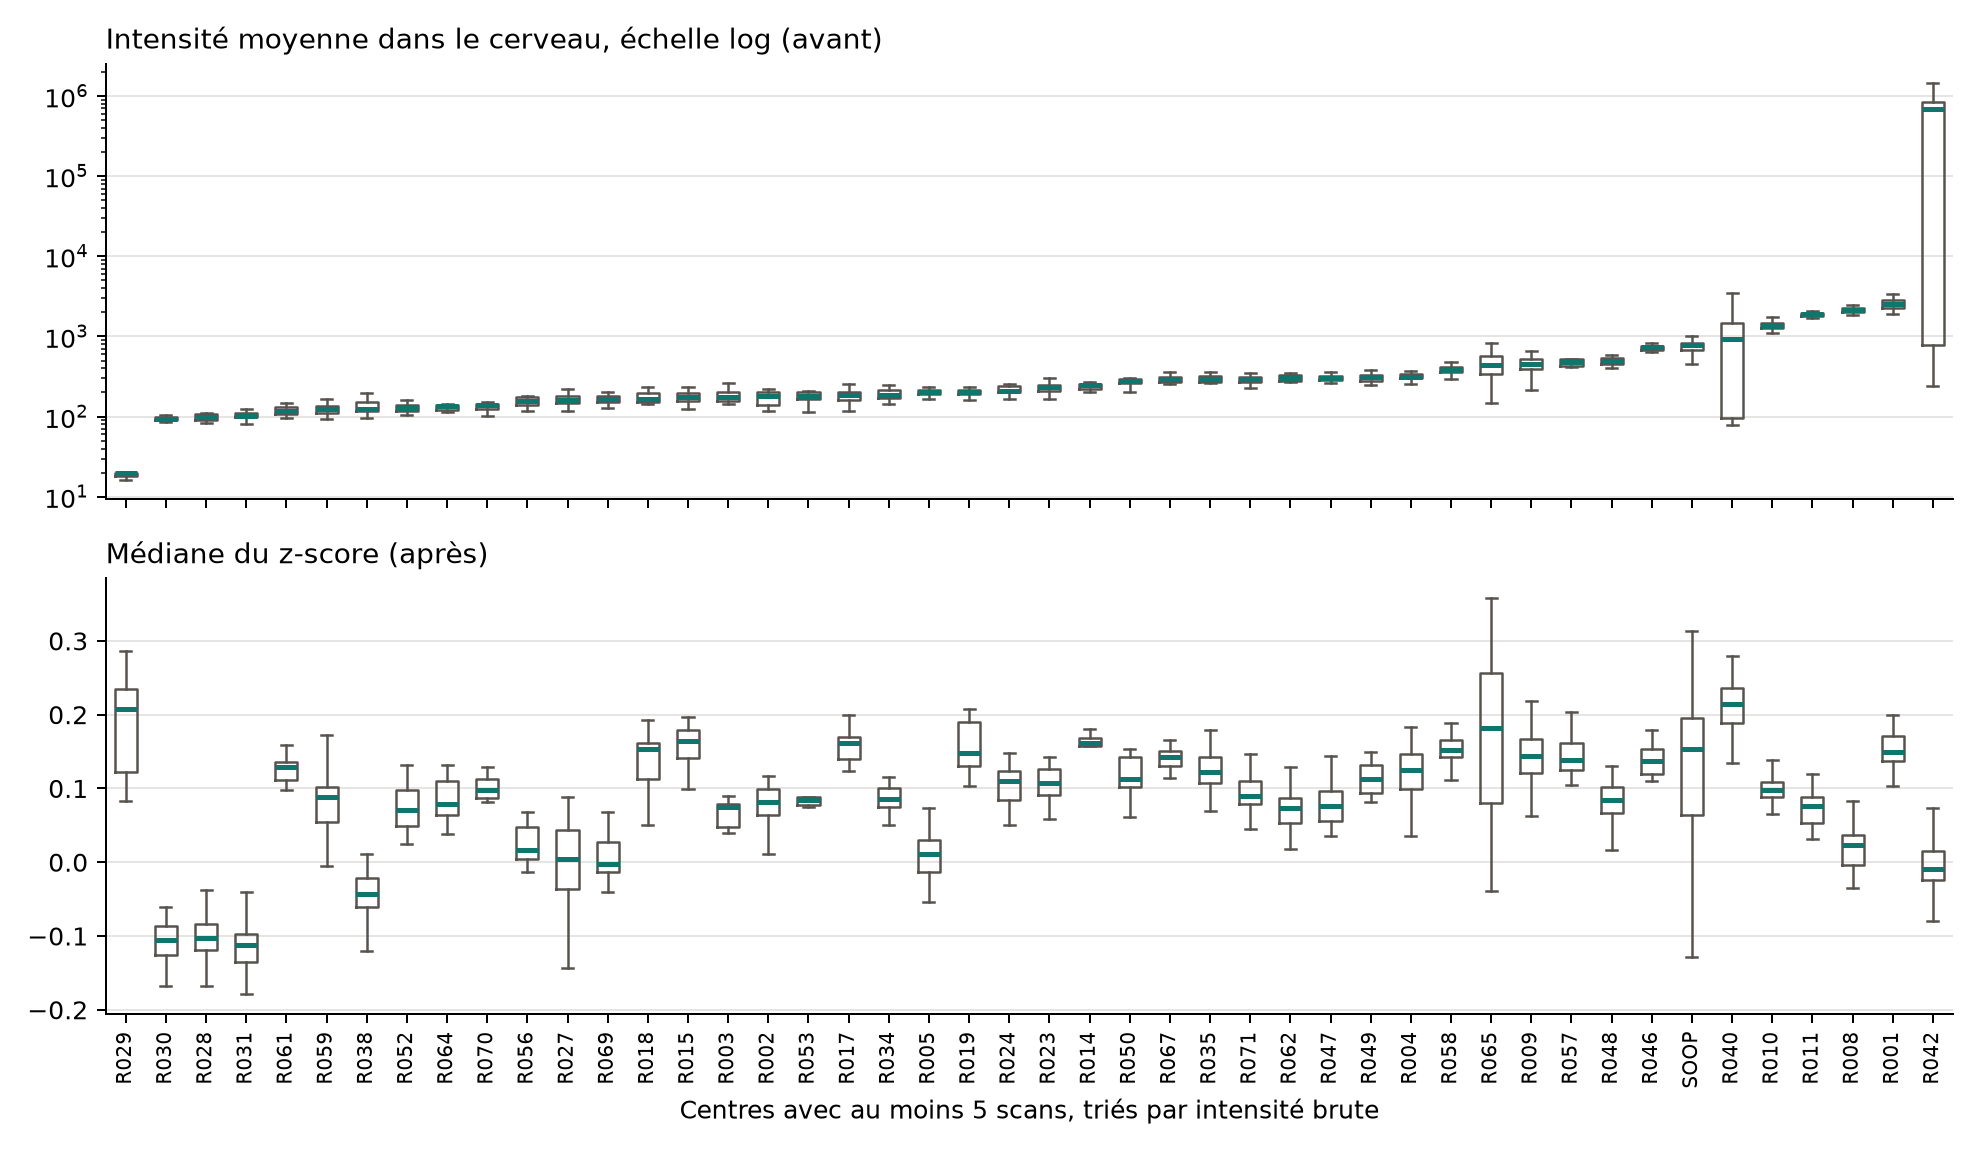
\includegraphics[angle=90,height=0.9\textheight]{figures/s5_avant_apres_par_centre.png}
  \caption{Intensité moyenne dans le cerveau avant prétraitement (échelle log) et médiane du z-score après, par centre (centres d'au moins 5 scans).}
  \label{fig:yosra-s5-avant-apres}
\end{figure}

\begin{figure}[htbp]
  \centering
  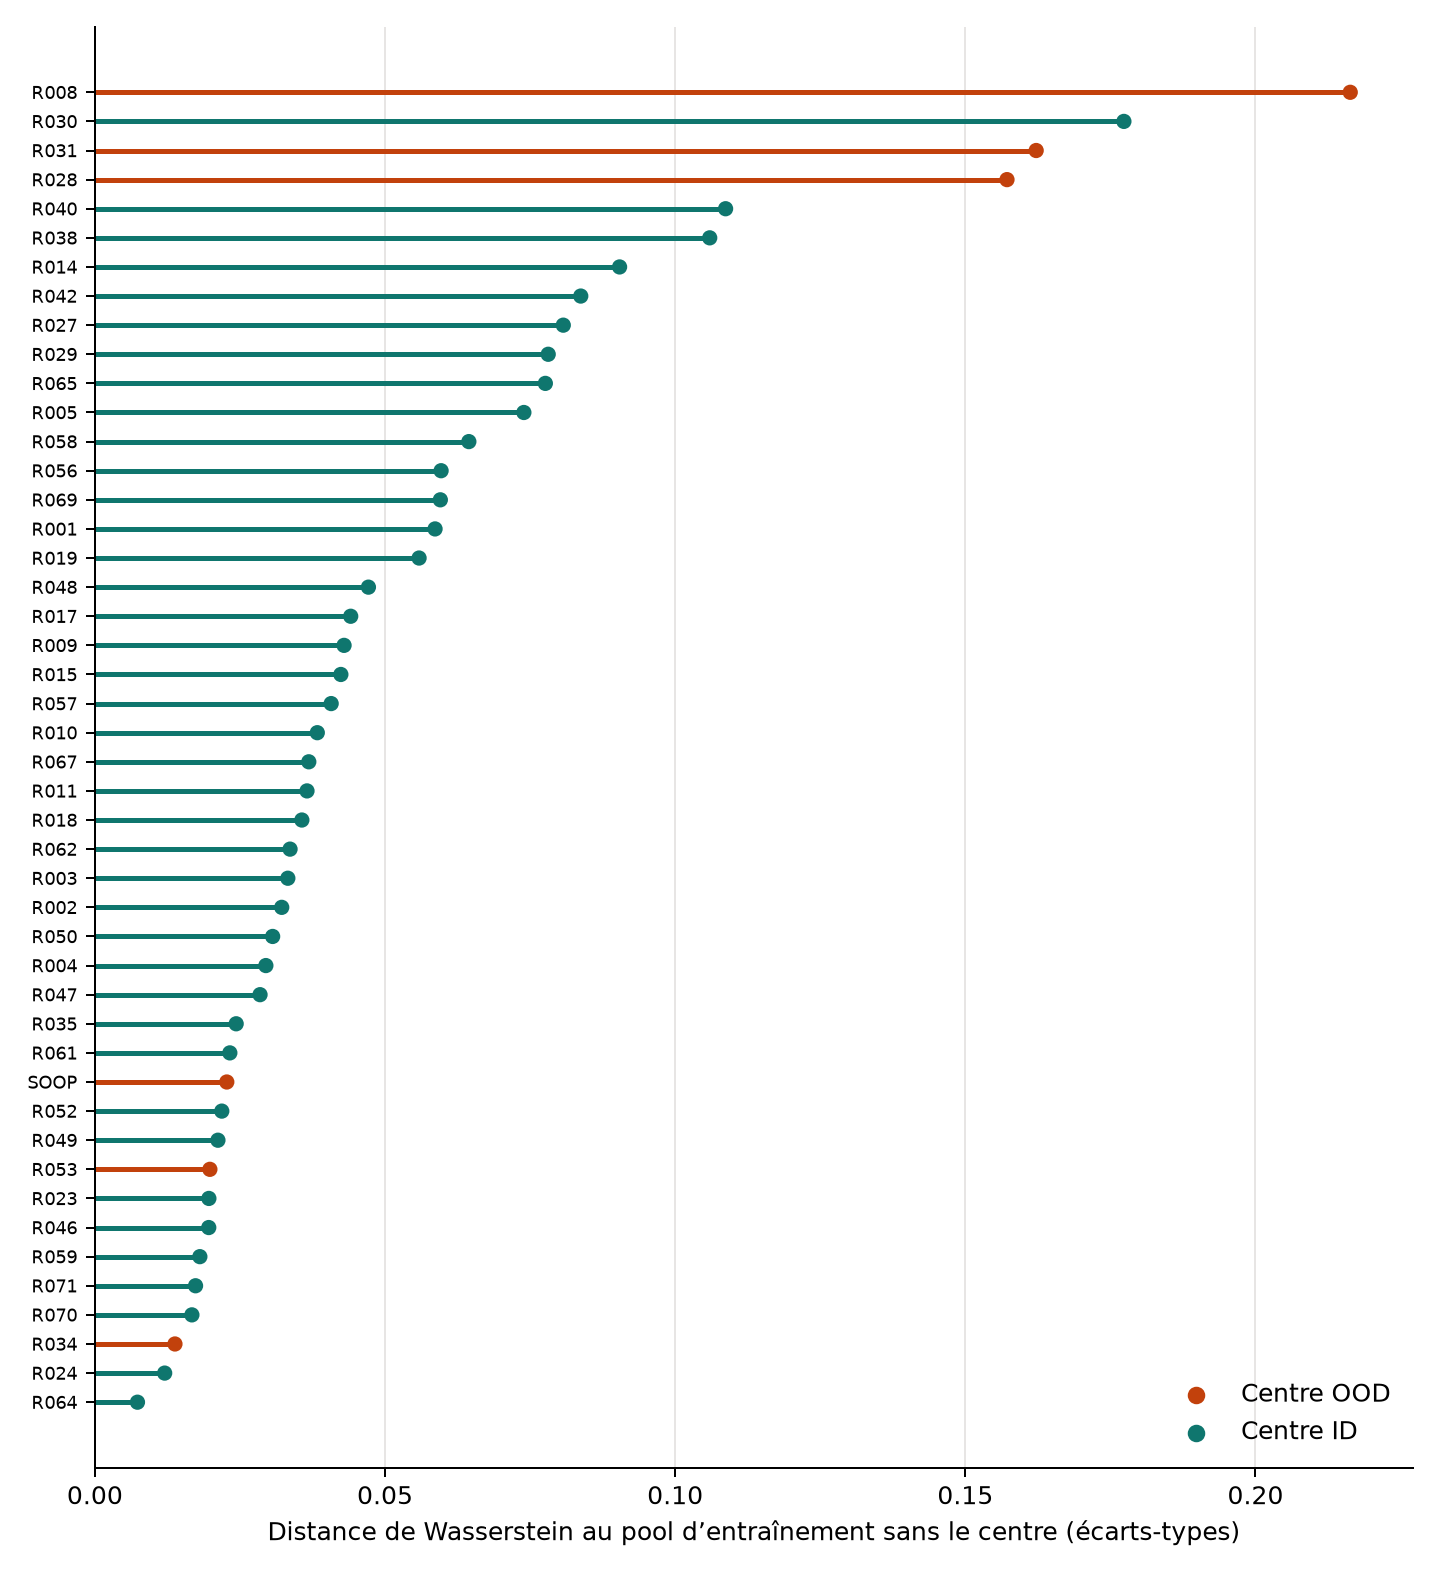
\includegraphics[width=0.85\linewidth]{figures/s5_distances_centres.png}
  \caption{Distance de Wasserstein de chaque centre au pool d'entraînement sans ce centre ; centres OOD en orange.}
  \label{fig:yosra-s5-distances}
\end{figure}

\begin{figure}[htbp]
  \centering
  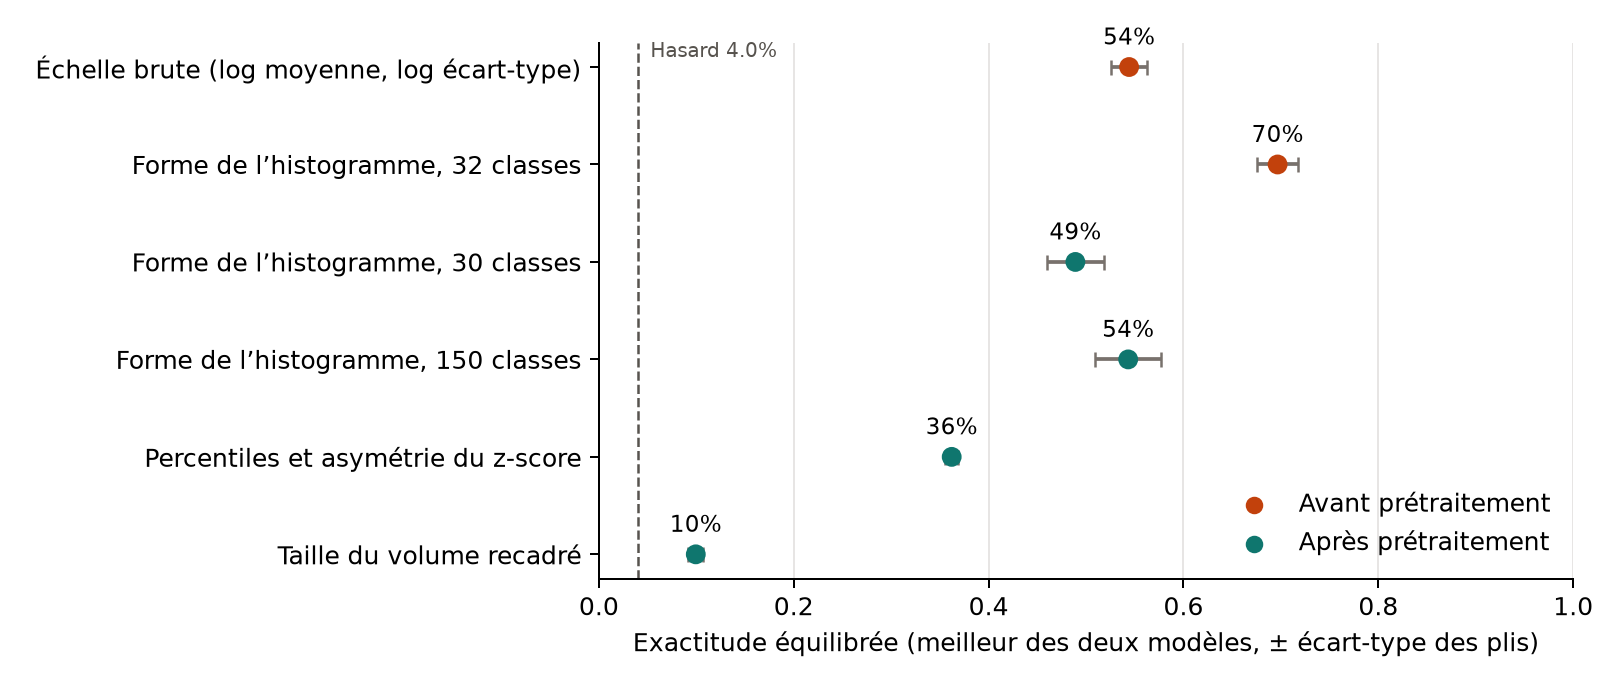
\includegraphics[width=\linewidth]{figures/s6_empreinte_centre.png}
  \caption{Empreinte du centre (S6) : exactitude équilibrée de la prédiction du centre selon la représentation, avant et après prétraitement (hasard : 4~\%).}
  \label{fig:yosra-s6}
\end{figure}

\section{Prédiction d'échec et effet du temps : protocole C1 préparé}
\label{sec:yosra-s7-s8}

S7 met en relation la distance au train du pli et l'erreur $1 - \mathrm{Dice}$ par centre.
Une validation leave-one-center-out produit des prédictions hors calibration.
La régression et le seuil d'alerte sont ajustés uniquement sur les autres centres de validation.
La différence de Dice par rapport au test ID est rapportée séparément.
Sans les résultats C3 de C1, ni corrélation empirique ni performance d'alerte ne peuvent être annoncées.

S8 compare les associations du centre et du délai post-AVC par modèles linéaires emboîtés sur les mêmes cas complets.
Le délai est transformé par $\log(1 + \textrm{jours})$.
Le test de permutation préserve le centre.
Les délais manquants, la sélection des cas et les confusions possibles limitent l'interprétation.
Le protocole n'établit pas une relation causale.

\section{Caractéristiques du réseau (C6 v2)}
\label{sec:yosra-c6}

La version C6 v2 mesure le décalage dans l'espace appris par le réseau plutôt que sur les
intensités. Le modèle C8 (U-Net 3D, augmentation d'intensité, pli 0) est gelé et utilisé en
mode évaluation, sans gradient et sans masque lésionnel. Pour chaque sujet, la sortie du
bottleneck, la couche que lit le classifieur de centre de DANN, est moyennée dans l'espace :
on obtient un vecteur de 320 valeurs par scan.
L'entrée est le volume C1 complet, complété par des zéros jusqu'à un multiple de 16. Le réseau
a été entraîné sur des patchs $96^3$ : sur le volume entier, les normalisations d'instance
portent sur une autre étendue. La même règle est appliquée à tous les scans, ce qui garde la
comparaison entre centres cohérente.

La comparaison d'empreinte baseline / augmentation / DANN demande les checkpoints baseline et
DANN du même protocole ; elle reste à faire.

\section{Démonstration et limites}
\label{sec:yosra-demo}

L'application Gradio affiche les coupes d'une IRM et un masque, calcule le volume lésionnel en mL et accepte une carte d'incertitude.
Un adaptateur permet de brancher le modèle final.
NiiVue fournit une vue 3D locale sur la route \texttt{/viewer/} du même serveur.
ANTsPy peut recaler un template MNI et transférer un atlas de labels ; une inspection visuelle demeure nécessaire avant de nommer les régions.

L'alerte individuelle d'intensité utilise un quantile de validation distinct du seuil par centre.
Elle n'est ni une garantie de performance ni une décision clinique.
En l'absence d'une entrée requise, l'application indique ce qui manque au lieu de créer un résultat.
Le support animé de secours est synthétique et explicitement étiqueté.

\subsection{Interface web du projet}
\label{sec:yosra-frontend}

Une application web (\texttt{frontend/}) présente l'ensemble du projet en dix pages :
vue d'ensemble, avancement du pipeline, contrôle qualité, prétraitement Spark, décalage entre
centres, modèles et Dice, adaptation de domaine, démonstration IRM avec vue 3D, conclusions
et galerie des figures. Le serveur FastAPI lit uniquement les rapports versionnés du dépôt
(\texttt{analysis/reports}, \texttt{preprocessing/reports}, \texttt{baselines/outputs},
\texttt{adaptation/outputs}, \texttt{integration/reports}) : aucun chiffre n'est simulé, et une
expérience absente est signalée comme telle. Chaque page et chaque carte indiquent qui a
produit le résultat. L'interface fonctionne sans étape de construction ni ressource externe ;
seules les figures des dossiers de résultats sont servies, jamais les données IRM. Sept tests
couvrent l'API (\texttt{frontend/tests/test\_server.py}).

\subsection{Branchement du modèle C8}
\label{sec:yosra-c8}

La démonstration (\texttt{demo/app.py}) et l'interface web appellent la fonction désignée par
la variable \texttt{AVC\_PREDICT\_ADAPTER}, au format \texttt{module:fonction}. L'adaptateur de
l'équipe, \texttt{adaptation.demo\_adapter:predict}, applique le prétraitement S4 puis le modèle
retenu (augmentation d'intensité, pli 0) et enregistre le masque en NIfTI \texttt{uint8} dans la
grille de l'IRM reçue. Il demande PyTorch et MONAI, absents de l'environnement de la
démonstration. Le pont \texttt{demo/c8\_bridge.py} lance donc cet adaptateur dans
l'environnement du modèle, dans un processus séparé, et récupère le masque ; la démonstration
utilise \texttt{AVC\_PREDICT\_ADAPTER=c8\_bridge:predict}. Le checkpoint est lu dans
\texttt{data/modeles/unet3d\_intensity\_pli0\_best.pt} (SHA-256 \texttt{ee6b93af\ldots abb6}),
hors du dépôt.

Sur le sujet OOD R034\_sub-r034s003\_ses-1, le rapport de la démonstration donne un volume
lésionnel de 27,058~mL (27\,058 voxels de 1~mm$^3$). Cette valeur concorde avec le volume
prédit lors de l'évaluation du modèle : 27,054~mL dans le fichier \texttt{resultats\_ood\_test.csv}
de la run intensité, conservé hors du dépôt. Sur le sujet OOD R031\_sub-r031s006\_ses-1, envoyé
sans masque à l'interface web, le modèle prédit 33,8~mL pour 27,7~mL annotés, soit un Dice de
0,745, en environ 35~s sur processeur. Ces deux cas vérifient le branchement ; ils ne constituent
pas une évaluation. Le modèle ne produit pas de carte d'incertitude. Cinq tests couvrent les
erreurs du pont (\texttt{tests/test\_c8\_bridge.py}).

\section{Discussion et travaux à terminer}
\label{sec:yosra-discussion}

Les principales limites actuelles sont la quarantaine QC à relire collectivement, le faible nombre de centres pour calibrer un prédicteur d'échec, la dépendance des distances aux effectifs, les métadonnées manquantes et l'absence locale des checkpoints et des Dice correspondant à C1 v2.
Les résultats RQ3 du pli 0 et le checkpoint C8 sont désormais disponibles (chapitre RQ3,
conclusion). Les analyses S7 et S8 sur C1 v2 attendent encore les Dice par sujet, y compris
sur la validation, qui sert à calibrer le seuil d'alerte sans consulter le test. L'empreinte
avant/après DANN attend les checkpoints baseline et DANN. La vidéo de vraie inférence et la
relecture collective restent à faire.
Une analyse S8 historique distincte est disponible plus bas (section~\ref{sec:yosra-s8-historique}).
Les références bibliographiques du document de projet doivent être vérifiées dans leurs publications originales avant d'être reprises dans la version remise.

\section{Compléments vérifiés de la livraison v2}
\label{sec:yosra-livraison}

L'export nnU-Net contient 916 images et labels d'entraînement, 499 images de test (231 ID, 268 OOD) et cinq plis (\nolinkurl{preprocessing/reports/export_v2.json}).
Le contrôle officiel nnU-Net reste à lancer dans l'environnement d'entraînement de Fayfa.
Les autres appartenances de v1 sont conservées.

L'analyse descriptive S8 trouve 1\,073 délais utilisables et 342 manquants ou invalides ; le délai médian est de 365 jours.
Huit centres n'ont aucun délai utilisable.
L'association centre / log-délai (eta carré 0,7475) souligne la nécessité de tenir compte du centre ; elle ne mesure pas l'effet du délai sur le Dice.
Voir \nolinkurl{analysis/reports/s8_metadata/} (\nolinkurl{summary.json}).

Le seuil individuel d'atypie du pli~0 vaut 0,114885 : référence de 733 scans du train, quantile 95~\% sur 183 scans de validation.
Aucun test ID/OOD n'a servi à ce réglage.
Le seuil est enregistré dans \texttt{data/demo/reference\_ood.json} (pli 0, quantile 0,95,
733 scans d'entraînement, 183 de validation), hors du dépôt comme l'ensemble de \texttt{data/}.

Chrome a chargé l'application, produit le rapport synthétique de 2,091~mL, puis affiché les coupes et le rendu 3D NiiVue sans erreur JavaScript (\nolinkurl{docs/pipeline/demo_verification/browser_report.json}).
L'image Docker a été construite et ses routes ainsi que le calcul du rapport ont été testés (\nolinkurl{docs/pipeline/verification.json}).
La vidéo de secours MP4 utilise ces captures réelles d'interface sur un phantom explicitement synthétique ; elle ne montre pas une inférence du réseau.

L'atlas Harvard-Oxford et le template compatible MNI152NLin6Asym ont été récupérés avec leurs sources et empreintes dans \nolinkurl{data/demo/atlas/provenance.json} (hors du dépôt ; copie versionnée : \nolinkurl{docs/pipeline/demo_verification/atlas_provenance.json}).
Les labels corticaux sont prioritaires, puis les labels sous-corticaux décalés de 100 ; les zones non couvertes gardent la valeur zéro.
Le recalage natif exige une relecture anatomique.
Sources : Nilearn Harvard-Oxford\footnote{\url{https://nilearn.github.io/stable/modules/generated/nilearn.datasets.fetch_atlas_harvard_oxford.html}} et TemplateFlow MNI152NLin6Asym\footnote{\url{https://github.com/templateflow/tpl-MNI152NLin6Asym}}.

Le recalage SyN sur l'exemple réel a été exécuté.
Atlas et IRM ont la même grille, les labels restent entiers et 97,75~\% des voxels atlas non nuls se trouvent dans le support d'intensité de l'image (\nolinkurl{docs/pipeline/verification.json}).
La planche locale \nolinkurl{data/demo/registration/qc_overlay.png} (hors du dépôt) a été examinée dans trois plans ; cela ne remplace pas une relecture anatomique experte.
Le rapport régional utilise le masque de référence fourni, sans inférence de réseau.

\section{S8 : résultat exploratoire sur les baselines récupérées}
\label{sec:yosra-s8-historique}

Le 12 novembre, les scores historiques de \texttt{cnn\_pretrained\_freeze-none} ont été rattachés à leur propre partition (903 train, 226 ID validation, 287 OOD), sans les reclasser dans C1 v2.
L'analyse utilise 167 cas ID complets de 31 centres et 257 cas OOD de 12 centres.
En ID, 58 délais manquent ou sont invalides et un Dice est absent ; en OOD, 30 délais manquent ou sont invalides.
Le Dice absent du cas à masque vide n'est pas remplacé par un score supposé.

Après ajustement sur le centre, l'ajout de $\log(1 + \textrm{délai})$ augmente le R$^2$ de 0,000046 en ID ($p$ exploratoire $= 0{,}911$) et de 0,03808 en OOD ($p = 0{,}001$ ; 999 permutations intra-centre pour chaque groupe).
Après ajout de $\log(1 + \textrm{volume lésionnel})$, ces gains sont respectivement 0,000711 et 0,000217 (\nolinkurl{analysis/reports/s8_historical/summary.json}).
L'association OOD dépend donc fortement des variables prises en compte ; elle ne permet pas d'attribuer un effet causal au temps.
Le volume est une analyse de sensibilité, pas un ajustement causal validé.
La figure~\ref{fig:yosra-s8} montre les cas utilisés.

\begin{figure}[htbp]
  \centering
  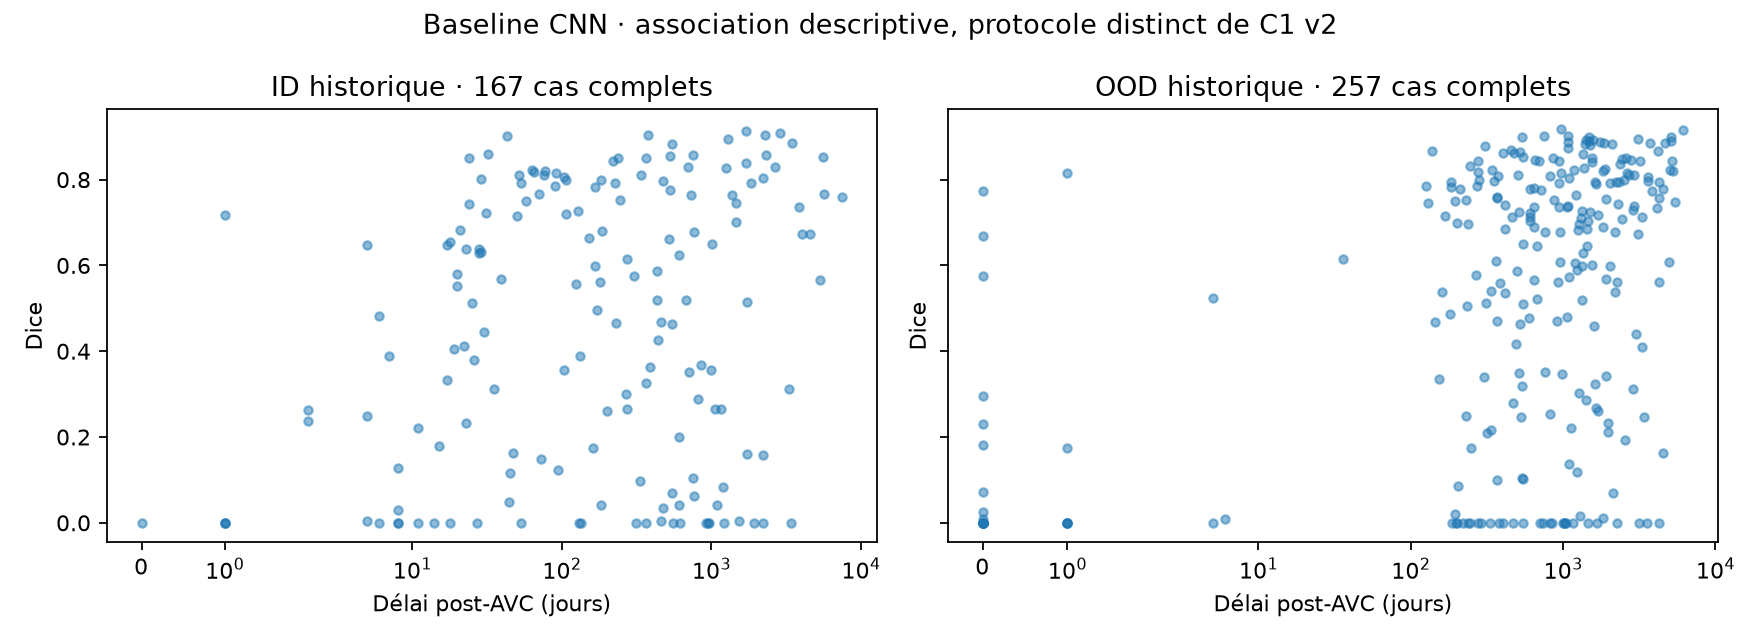
\includegraphics[width=\linewidth]{analysis/reports/s8_historical/time_dice.png}
  \caption{Dice de la baseline CNN historique selon le délai post-AVC, cas complets ID (167) et OOD (257) ; protocole distinct de C1 v2.}
  \label{fig:yosra-s8}
\end{figure}

Ces deux tests sont exploratoires, sans correction de multiplicité.
L'ID a participé au choix historique du modèle et n'est pas un test indépendant.
La partition et le prétraitement diffèrent de C1 v2.
Les résultats des autres baselines sont résumés séparément sur leurs effectifs disponibles, sans comparaison appariée implicite.

Livrables reproductibles : \nolinkurl{analysis/historical_baselines.py}, \nolinkurl{analysis/reports/s8_historical/summary.json}, \nolinkurl{README.md}, \nolinkurl{model_summary.csv}, \nolinkurl{missing_by_center.csv} et \nolinkurl{time_dice.png}.
Les empreintes des fichiers sources sont conservées.

\section{S6 : complément sur l'incertitude}
\label{sec:yosra-s6-incertitude}

Une évaluation complémentaire utilise 912 sujets d'entraînement et 228 sujets réservés, stratifiés parmi les mêmes 25 centres.
Deux classifieurs fixés, régression logistique et forêt aléatoire, sont évalués sur les mêmes sujets.
Les sujets réservés sont ensuite rééchantillonnés 10\,000 fois à l'intérieur de chaque centre, avec les mêmes indices pour toutes les représentations ; l'exactitude équilibrée donne le même poids aux centres.

Pour la forêt aléatoire, le score avant traitement (32 classes) est de 70,1~\%, avec un intervalle percentile conditionnel à 95~\% de [64,6 ; 75,5]~\%.
Après traitement (30 classes), il est de 51,1~\% [45,3 ; 57,0]~\%.
La différence appariée après moins avant est de $-19{,}0$ points [$-25{,}5$ ; $-12{,}6$].
Pour la régression logistique, elle est de $-21{,}5$ points [$-27{,}4$ ; $-15{,}5$] (\nolinkurl{analysis/reports/s6_uncertainty/intervals.csv}, \nolinkurl{analysis/reports/s6_uncertainty/paired_differences.csv}).
La variante après traitement à 150 classes est aussi rapportée pour montrer la sensibilité à la représentation, sans sélectionner uniquement le meilleur score.
La figure~\ref{fig:yosra-s6-incertitude} présente ces intervalles.

\begin{figure}[htbp]
  \centering
  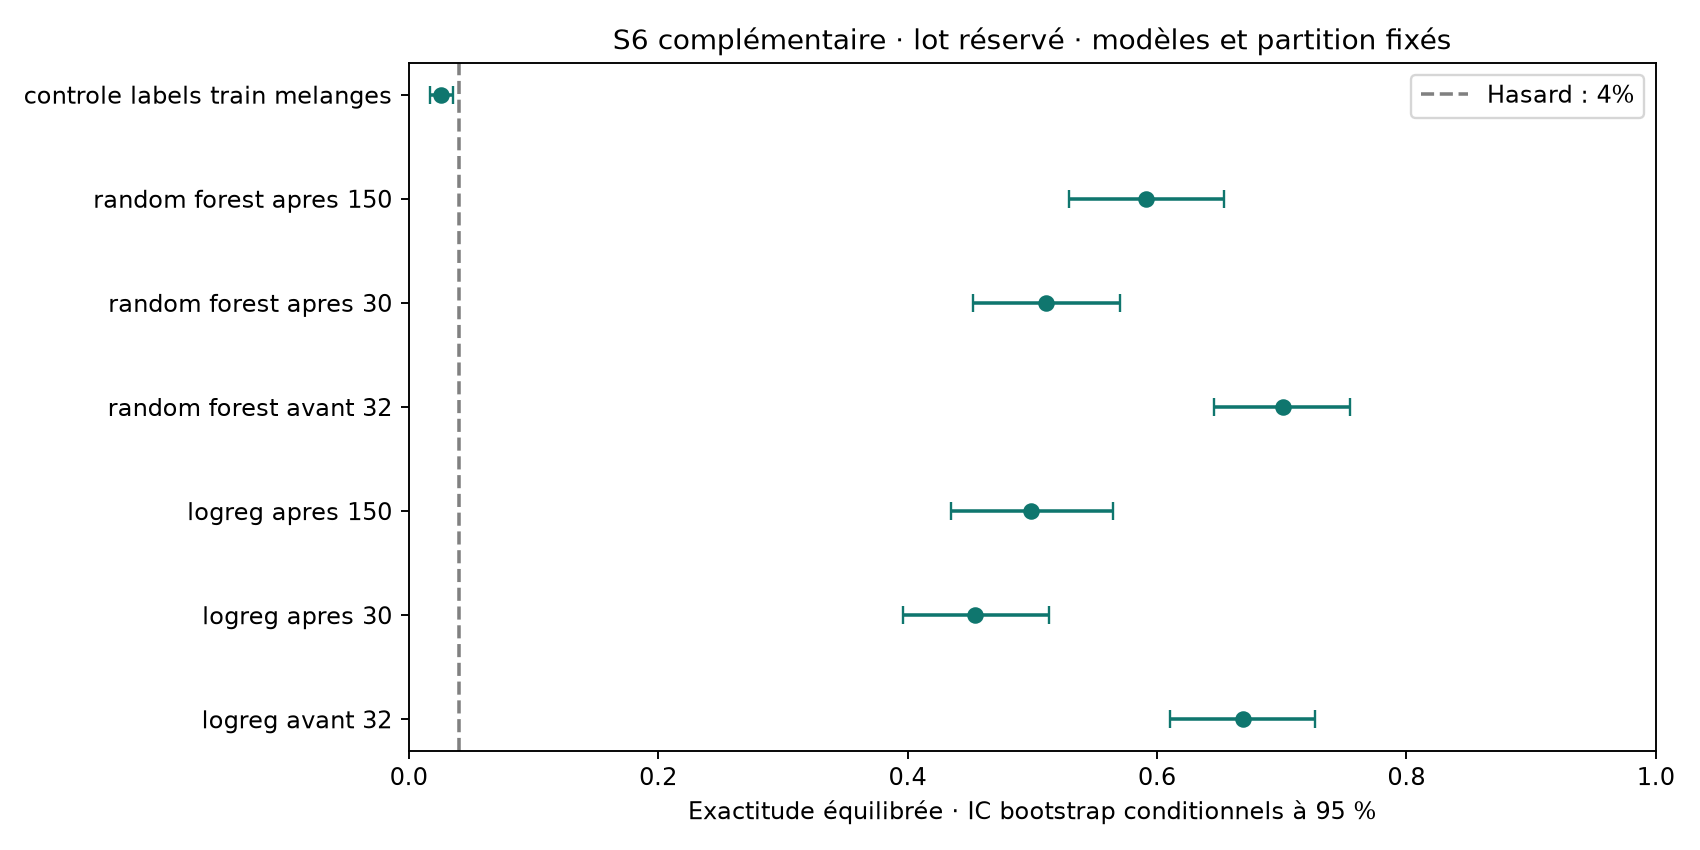
\includegraphics[width=\linewidth]{analysis/reports/s6_uncertainty/confidence_intervals.png}
  \caption{Exactitude équilibrée de la reconnaissance du centre sur le lot réservé, avec IC bootstrap conditionnels à 95~\% (modèles et partition fixés).}
  \label{fig:yosra-s6-incertitude}
\end{figure}

Ces intervalles conditionnent sur les modèles et la partition fixés : ils n'incluent pas la variabilité d'un nouvel entraînement.
La cohorte avait déjà été explorée en S6, et la granularité avant/après reste différente.
Il s'agit d'un complément exploratoire, pas d'une validation externe ni d'un effet causal isolé du prétraitement.
Les centres sont présents dans le train et le test : l'expérience mesure leur reconnaissance, pas la segmentation dans un centre inconnu.
Les moyennes des cinq plis précédentes restent inchangées et ne doivent pas être confondues avec ces nouveaux scores.

Livrables : \nolinkurl{analysis/reports/s6_uncertainty/README.md}, \nolinkurl{intervals.csv}, \nolinkurl{paired_differences.csv}, \nolinkurl{summary.json} et \nolinkurl{confidence_intervals.png}.
Les prédictions individuelles restent dans \nolinkurl{data/analysis/s6_uncertainty/} (hors du dépôt).

\section{Synthèse du contrôle qualité par centre}
\label{sec:yosra-qc}

La synthèse couvre les 1\,453 sujets inventoriés dans 55 centres.
Elle retrouve 1\,415 sujets retenus dans 54 centres, 38 exclus et aucune erreur active.
Les exclusions correspondent aux 37 cas R032 pour espacement non fiable et au cas R065 mis en quarantaine pour annotation hors du support et du recadrage.
Cette synthèse n'ajoute aucune exclusion et ne remplace pas la relecture collective des décisions.

Parmi les 1\,415 sujets retenus, cinq masques sont vides et conservés comme cas négatifs ; 1\,410 sont non vides et aucun statut de masque n'est inconnu.
Le délai post-AVC est disponible pour 1\,073 sujets ; 342 délais sont manquants ou invalides (24,2~\%).
Huit centres retenus n'ont aucun délai utilisable.
Le drapeau CHRONICITY est présent pour 296 sujets et non renseigné pour 1\,119 ; cette absence ne permet pas de déduire un stade clinique.
Deux sujets SOOP portent l'avertissement de fichier de métadonnées vide : cet avertissement de fichier ne recouvre pas toutes les valeurs de délai absentes.

Les effectifs d'exclusion utilisent tout l'inventaire ; les pourcentages de métadonnées utilisent seulement les sujets retenus de chaque centre.
Pour R032, sans sujet retenu, les taux sont non définis plutôt que nuls.
Les colonnes inconnues ne sont pas assimilées à des masques non vides.
Le tableau détaillé, la figure, les motifs d'exclusion et les avertissements sont disponibles dans \nolinkurl{analysis/reports/qc_by_center/} (\nolinkurl{summary.json}, \nolinkurl{qc_by_center.csv}, \nolinkurl{exclusion_reasons.csv}, \nolinkurl{metadata_warnings.csv}).
% La figure qc_by_center.png (55 centres sur trois panneaux) n'est pas insérée : à la largeur de la page, son texte
% ferait environ 3 pt. Elle reste disponible dans analysis/reports/qc_by_center/.
\section{Vérification de l'intégration}
\label{sec:yosra-verification}

Après la fusion des contributions de l'équipe dans \texttt{main}, 310 tests réussissent :
50 pour le pipeline et les analyses, 7 pour l'interface web, 224 pour la généralisation et
l'adaptation (dont des patchs C1 réels) et 29 pour la calibration. Quatorze tests
d'entraînement (\texttt{adaptation/tests/test\_train.py}, \texttt{test\_continual.py}) échouent
sur le Mac de vérification : \texttt{torch.amp.GradScaler} n'existe pas dans torch 2.2.2,
dernière version disponible pour macOS Intel. L'entraînement est exécuté sur Kaggle ;
l'inférence du checkpoint C8 est vérifiée localement
(\texttt{integration/reports/verification.json}).

\setlength{\emergencystretch}{0pt}
. Version LaTeX de docs/pipeline/RAPPORT.md (commit 4540d85) :
% plan, contenu et formulations conservés ; chemins des fichiers sources ajoutés pour chaque chiffre.
% Paquets attendus dans le préambule : babel (french), graphicx, booktabs, makecell, hyperref, float.
% Réglages à mettre dans le préambule du rapport final :
%   \addto\captionsfrench{\def\tablename{Tableau}}   % « Tableau » au lieu de « Table »
%   \hypersetup{hidelinks}                             % liens sans cadre rouge
% Les chemins des figures sont relatifs à la racine du dépôt.
% Statut d'origine (RAPPORT.md) : brouillon scientifique fondé sur les résultats locaux disponibles ; les valeurs
% finales doivent être prises dans les JSON/CSV générés après le dernier QC ; les expériences sans prédictions ou
% checkpoints ne sont pas présentées comme réalisées.

% Chemins de fichiers longs : coupures de ligne aussi permises après « _ » et « - » dans \nolinkurl et \url.
\makeatletter
\g@addto@macro\UrlBreaks{\do\_\do\-}
\makeatother
% Étirement d'urgence limité à ce chapitre (lignes chargées de chemins), remis à zéro à la fin.
\setlength{\emergencystretch}{3em}

\chapter{Données, décalage de domaine et démonstration}
\label{chap:yosra}

\section{Introduction et questions de recherche}
\label{sec:yosra-introduction}

Ce projet étudie la segmentation des lésions d'AVC sur des IRM T1 acquises dans plusieurs centres.
Les différences de scanner, protocole et résolution peuvent modifier la distribution des images.
Notre objectif est de mesurer ce décalage, d'évaluer la généralisation des modèles sur des centres absents de l'entraînement, puis d'étudier la possibilité d'anticiper et de réduire leur perte de performance.

Trois questions structurent le projet : quel est l'écart entre test ID et test OOD ?
Les architectures Transformer améliorent-elles la généralisation par rapport à nnU-Net ?
Quelles techniques de généralisation ou d'adaptation réduisent cet écart ?
La contribution de Yosra fournit le pipeline de données, les partitions communes, les mesures du décalage, les analyses explicatives et l'interface de démonstration.
Les comparaisons de segmentation et l'adaptation continue sont produites par Fayfa et Anas.

\section{Données et contrôle qualité}
\label{sec:yosra-donnees}

L'inventaire local contient 1\,453 paires IRM/masque dans 55 centres.
Le centre R032, soit 37 cas, est exclu provisoirement pour espacement incohérent.
Les métadonnées vides sont signalées sans supprimer une paire utilisable.
Les masques vides sont conservés comme cas négatifs.
Le délai post-AVC reste numérique ; \texttt{CHRONICITY}, codé 1/vide, n'est pas interprété comme une catégorie aigu/subaigu/chronique
(\nolinkurl{analysis/reports/qc_by_center/summary.json}, \nolinkurl{analysis/reports/qc_by_center/exclusion_reasons.csv}).

La livraison v2 contient 1\,415 volumes prétraités, relus et exportés.
Elle exclut les 37 cas R032 et met un cas supplémentaire en quarantaine technique.
Le split v1 est archivé ; v2 retire uniquement ce cas, sans déplacer les autres sujets ni les centres.
La relecture collective de cette quarantaine reste nécessaire ; les annotations brutes sont intactes
(\nolinkurl{preprocessing/reports/release_v2.json}, \nolinkurl{preprocessing/qc_exclusions.json}).

\section{Pipeline Spark}
\label{sec:yosra-pipeline}

Chaque sujet constitue une unité de travail.
Le pipeline réoriente les images en RAS, rééchantillonne à 1~mm isotrope (linéaire pour l'image, plus proche voisin pour les masques), normalise les intensités dans le support cérébral et recadre avec une marge de cinq voxels.
Le support est défini par les intensités supérieures à la valeur de fond estimée ; cette précaution traite notamment le centre R029 dont le fond n'est pas nul.
Cette heuristique reste une limite et doit être examinée sur les cas atypiques.

Le z-score est stocké en \texttt{int16} avec un pas de 0,001.
L'erreur d'arrondi est au plus 0,0005 unité de z-score.
Le validateur utilise cette borne, avec une petite marge numérique, pour la moyenne et l'écart-type ; le fond doit rester exactement nul.
Une signature des entrées et paramètres permet la reprise et chaque paire est accompagnée d'un QC (\nolinkurl{preprocessing/week4.py}).

La boîte de recadrage est déterminée par l'image seule.
Le code existant tolère la suppression de labels hors boîte jusqu'à 1~\% du volume lésionnel.
Ce choix n'est pas une correction clinique des annotations : il doit être documenté et validé.
Le dernier cas dépasse cette tolérance (1,76~\% : 77 voxels sur 4\,376, \nolinkurl{preprocessing/qc_exclusions.json}) et est mis en quarantaine dans v2.
L'option N4 a été ajoutée pour une expérience distincte ; elle n'a pas été appliquée au jeu de référence et aucun bénéfice n'en est revendiqué.

\section{Partitions et absence de fuite}
\label{sec:yosra-partitions}

Le fichier commun \nolinkurl{splits.json} version 2 fixe 916 cas d'entraînement/validation, 231 cas ID et 268 cas OOD (\nolinkurl{preprocessing/reports/release_v2.json}).
Six centres OOD sont intégralement retirés : R008, R028, R031, R034, R053 et SOOP.
Les cinq plis séparent les centres d'entraînement et de validation.
Le test ID de chaque pli est limité aux centres présents dans son entraînement.
Le découpage compte 231 sujets ID au total ; pour le pli~0, le test ID n'en garde que 185, car les 46 autres appartiennent aux centres de validation de ce pli, absents de son entraînement (\nolinkurl{splits.json}, \texttt{folds[0].id\_test}).

La sélection des centres OOD varie taille et distance d'intensité.
Comme la distance participe à cette sélection, un écart de distance ID/OOD n'est pas une découverte indépendante.
Les mesures prédictives doivent utiliser la référence d'entraînement du modèle considéré, pas le pool global.
Aucun hyperparamètre d'alerte ne doit être choisi sur le test OOD.

\section{Benchmark}
\label{sec:yosra-benchmark}

Le pilote existant porte sur huit petits volumes et un essai par configuration.
Les temps de calcul sont 56,59~s, 41,46~s, 27,63~s et 42,54~s pour 1, 2, 4 et 8 workers.
L'accélération maximale mesurée est $\times$2,05 avec quatre workers (\nolinkurl{preprocessing/reports/benchmark_summary.csv}, \nolinkurl{preprocessing/reports/benchmark_scope.json}).
La dégradation à huit workers est compatible avec des coûts de concurrence et de ressources ; ce pilote ne permet pas d'en isoler la cause.
Les workers ne constituent pas des cœurs physiques réservés.
Le démarrage Spark n'entre pas dans \texttt{compute\_seconds}.
Les courbes ne sont pas extrapolées au dataset entier.
La figure~\ref{fig:yosra-benchmark} montre l'accélération mesurée.

\begin{figure}[htbp]
  \centering
  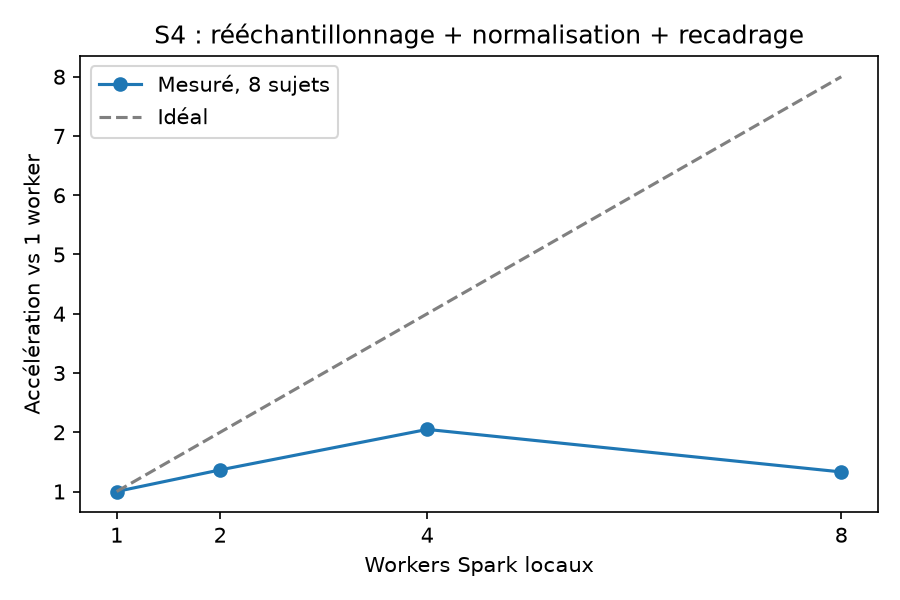
\includegraphics[width=0.6\linewidth]{preprocessing/reports/benchmark_speedup.png}
  \caption{Accélération du prétraitement S4 selon le nombre de workers Spark locaux (8 sujets, un essai).}
  \label{fig:yosra-benchmark}
\end{figure}

\section{Statistiques et empreinte du centre}
\label{sec:yosra-s5-s6}

Les rapports S5 comparent les distributions avant/après prétraitement et mesurent les distances Wasserstein et MMD entre centres et référence.
Le z-score contraint moyenne et variance par scan ; les différences restantes portent donc surtout sur la forme des distributions.
Les échelles avant/après ne sont pas identiques : leur comparaison normalisée reste descriptive.

Le test S6 prédit le centre depuis des histogrammes ou statistiques, avec cinq plis stratifiés, exactitude équilibrée et contrôle à labels mélangés.
Comparer des histogrammes de granularité proche et les mêmes patients permet de mieux isoler l'effet du prétraitement.
Une empreinte reconnaissable n'implique pas à elle seule une baisse du Dice.

Valeurs et figures : \nolinkurl{analysis/reports/post_stats_summary.json}, \nolinkurl{analysis/reports/site_fingerprint_s6.csv}, figures~\ref{fig:yosra-s5-avant-apres}, \ref{fig:yosra-s5-distances} et~\ref{fig:yosra-s6}.
Les versions historiques sur 1\,402 cas ne doivent pas être confondues avec la relance sur 1\,415.
Les versions historiques sur 1\,402 cas sont conservées dans l'historique Git du dépôt
(commit \texttt{5a86471}, fichier \texttt{analysis/reports/post\_stats\_summary.json}).

La relance du 11 novembre couvre 1\,415 sujets dans 54 centres.
La distance relative médiane passe de 0,1315 avant à 0,0376 après, sur la même cohorte disponible.
La corrélation entre Wasserstein et MMD vaut 0,842 pour les centres d'au moins cinq scans.
La médiane de Wasserstein vaut 0,0376 pour ID et 0,0900 pour OOD ; cet écart reste affecté par la sélection initiale des centres (\nolinkurl{analysis/reports/post_stats_summary.json}).
Le test S6 retient 1\,140 scans de 25 centres.
Avec les histogrammes 32 classes avant / 30 classes après et le meilleur des deux classifieurs, l'exactitude équilibrée vaut 69,7~\% puis 48,9~\%.
Le contrôle mélangé vaut 4,0~\%, proche du hasard à 4~\% (\nolinkurl{analysis/reports/site_fingerprint_s6.csv}, \nolinkurl{analysis/reports/site_fingerprint_s6_summary.json}).
Ces chiffres ne mesurent pas la performance de segmentation.

\begin{figure}[p]
  \centering
  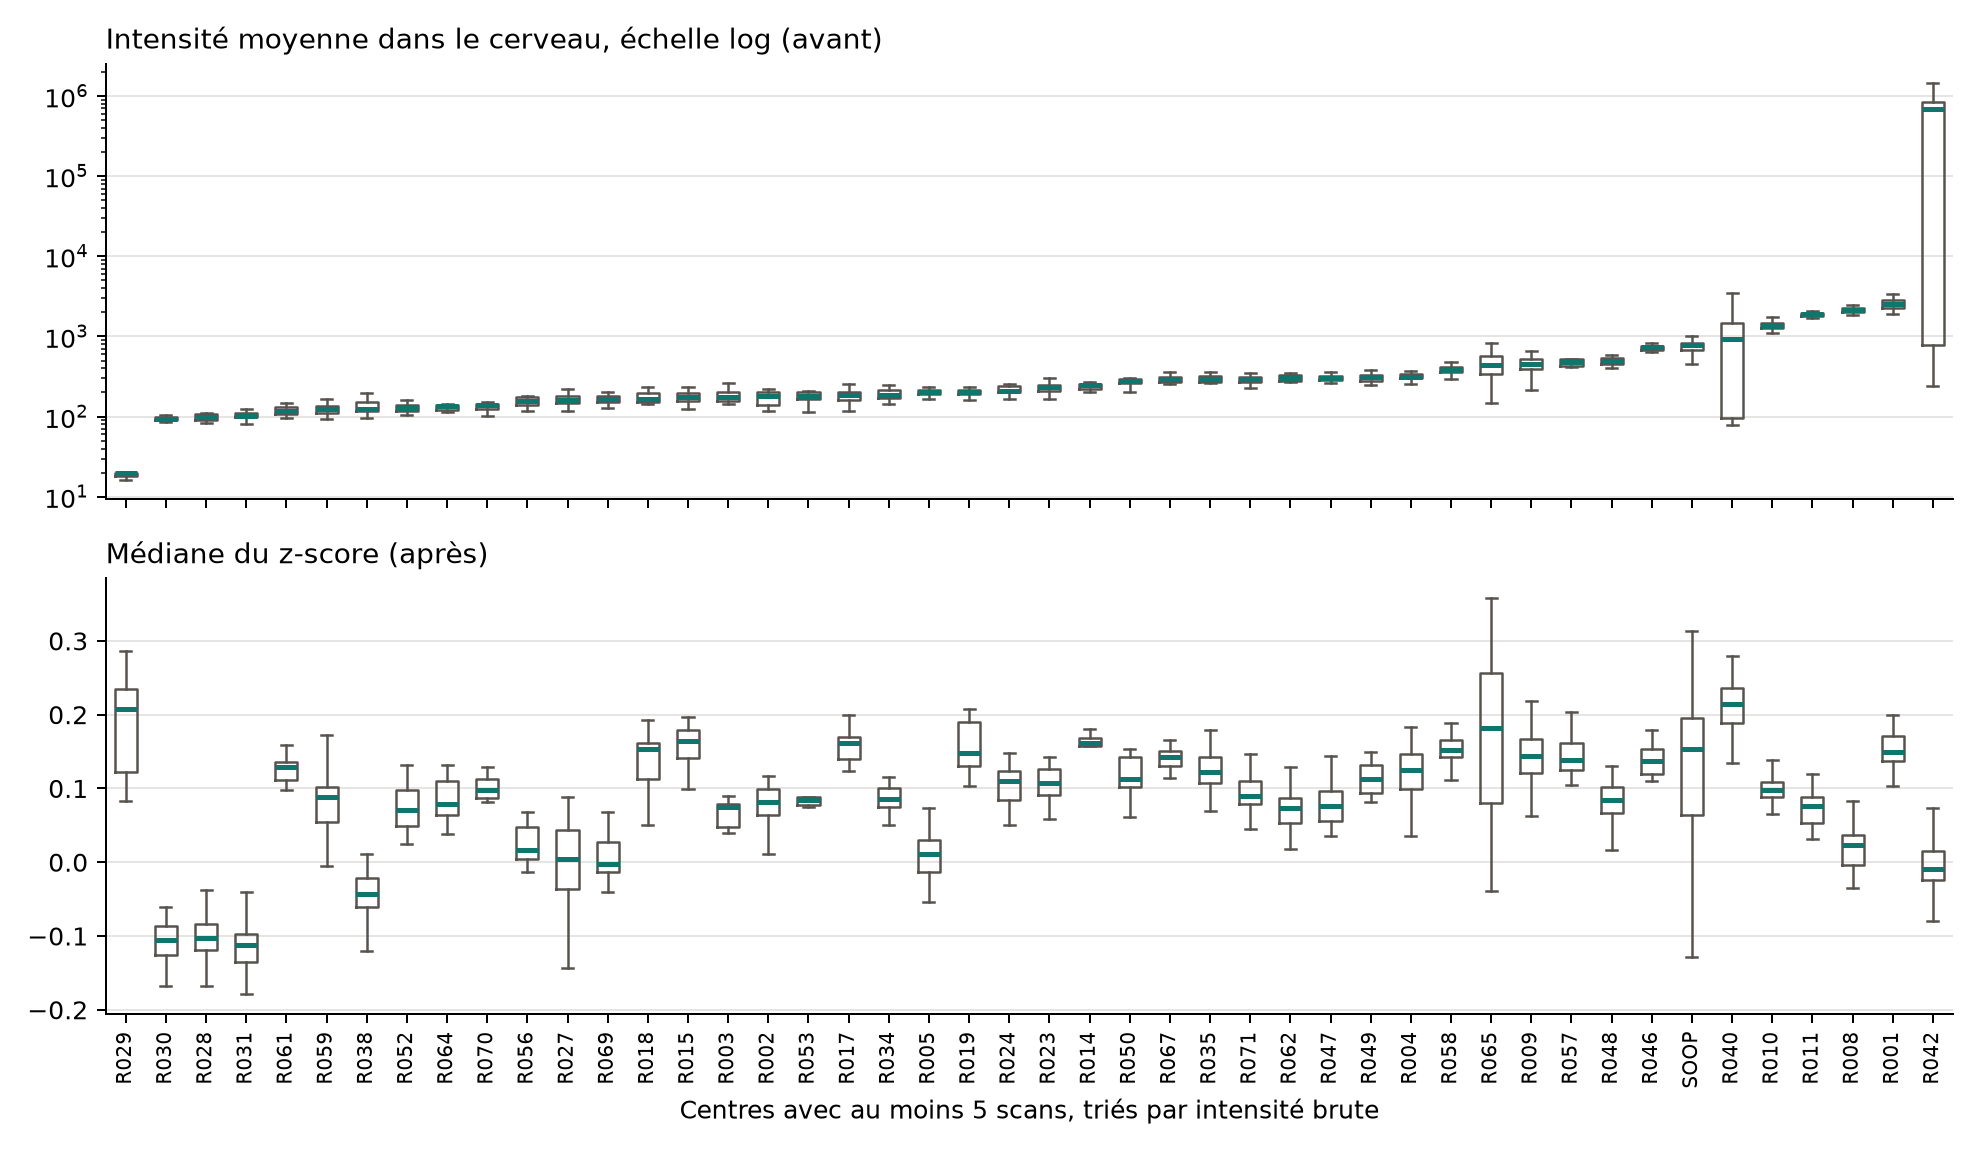
\includegraphics[angle=90,height=0.9\textheight]{figures/s5_avant_apres_par_centre.png}
  \caption{Intensité moyenne dans le cerveau avant prétraitement (échelle log) et médiane du z-score après, par centre (centres d'au moins 5 scans).}
  \label{fig:yosra-s5-avant-apres}
\end{figure}

\begin{figure}[htbp]
  \centering
  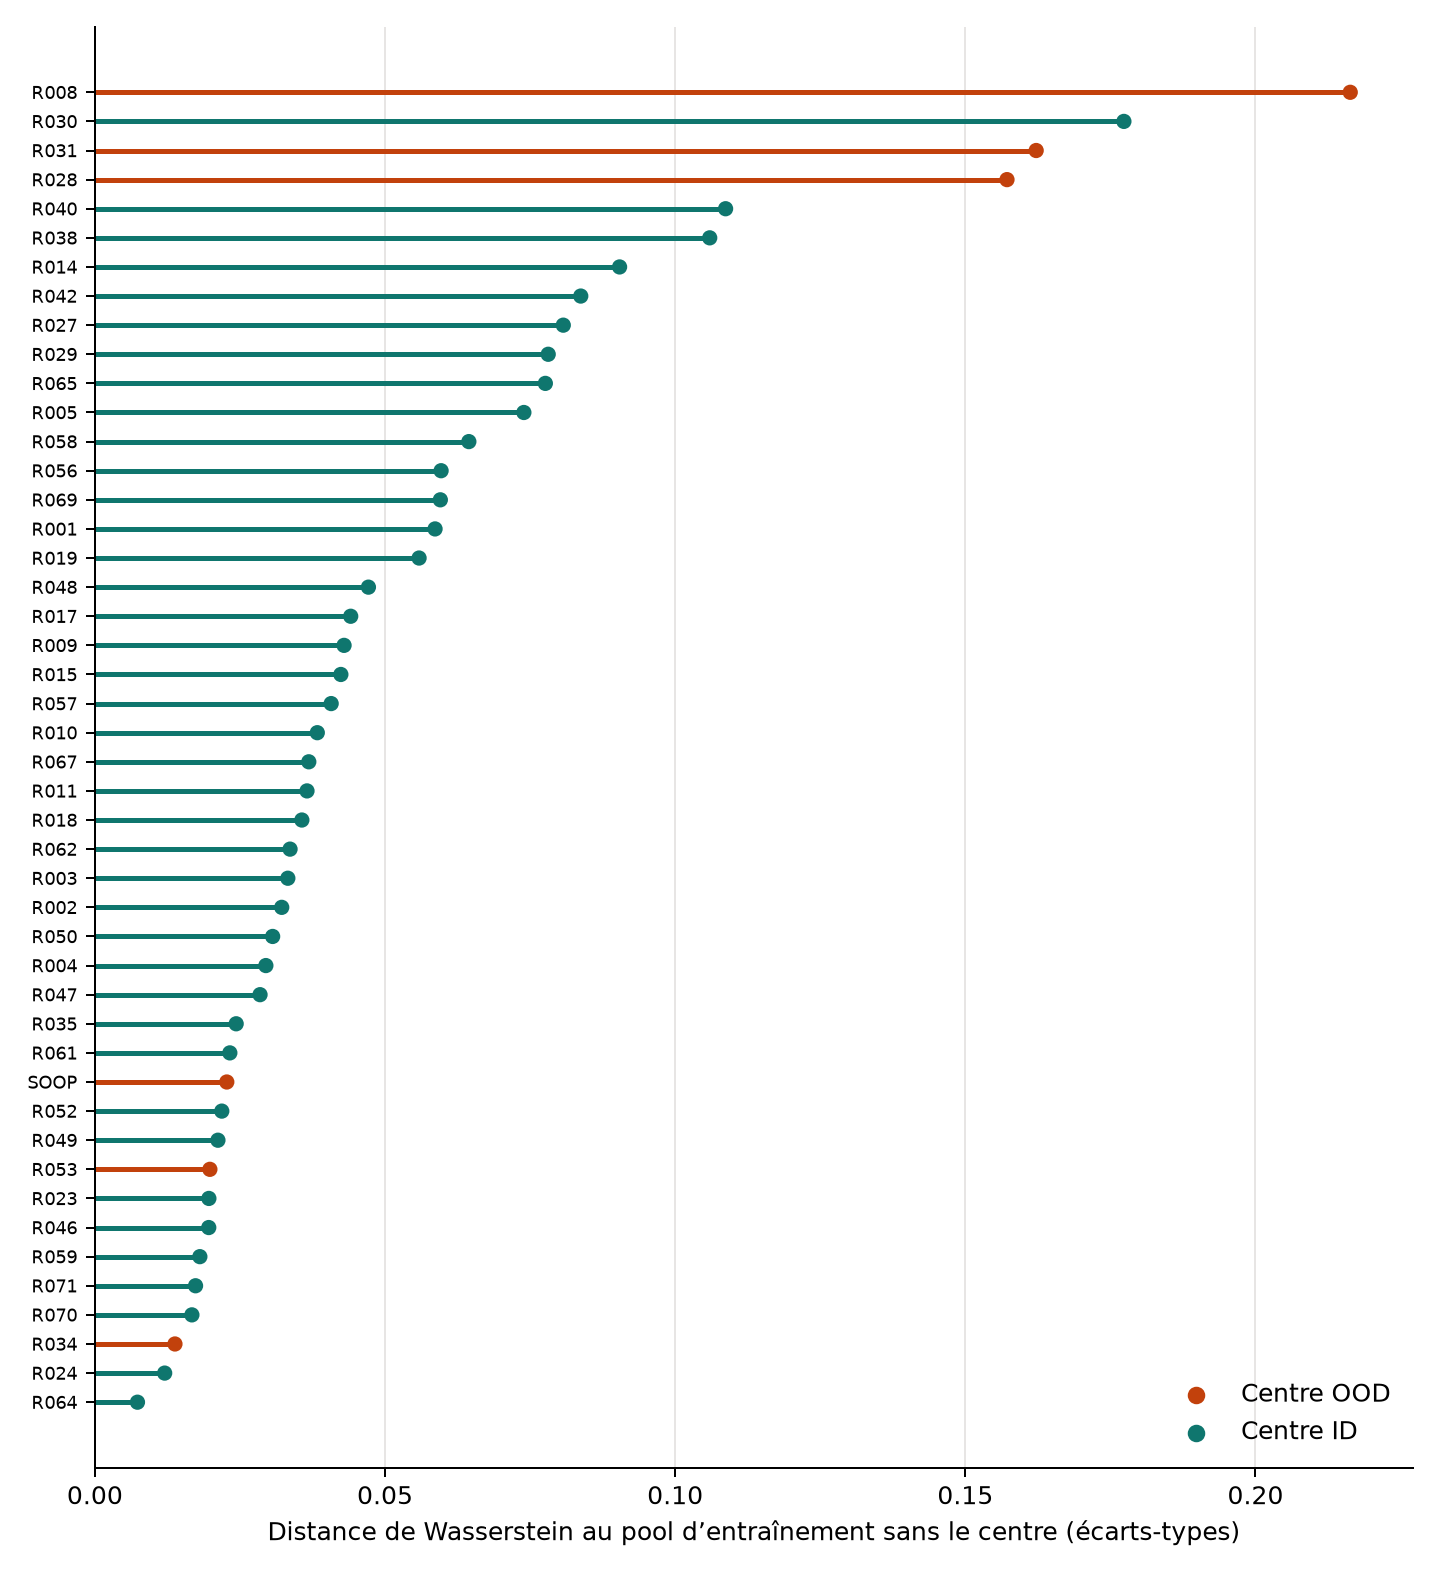
\includegraphics[width=0.85\linewidth]{figures/s5_distances_centres.png}
  \caption{Distance de Wasserstein de chaque centre au pool d'entraînement sans ce centre ; centres OOD en orange.}
  \label{fig:yosra-s5-distances}
\end{figure}

\begin{figure}[htbp]
  \centering
  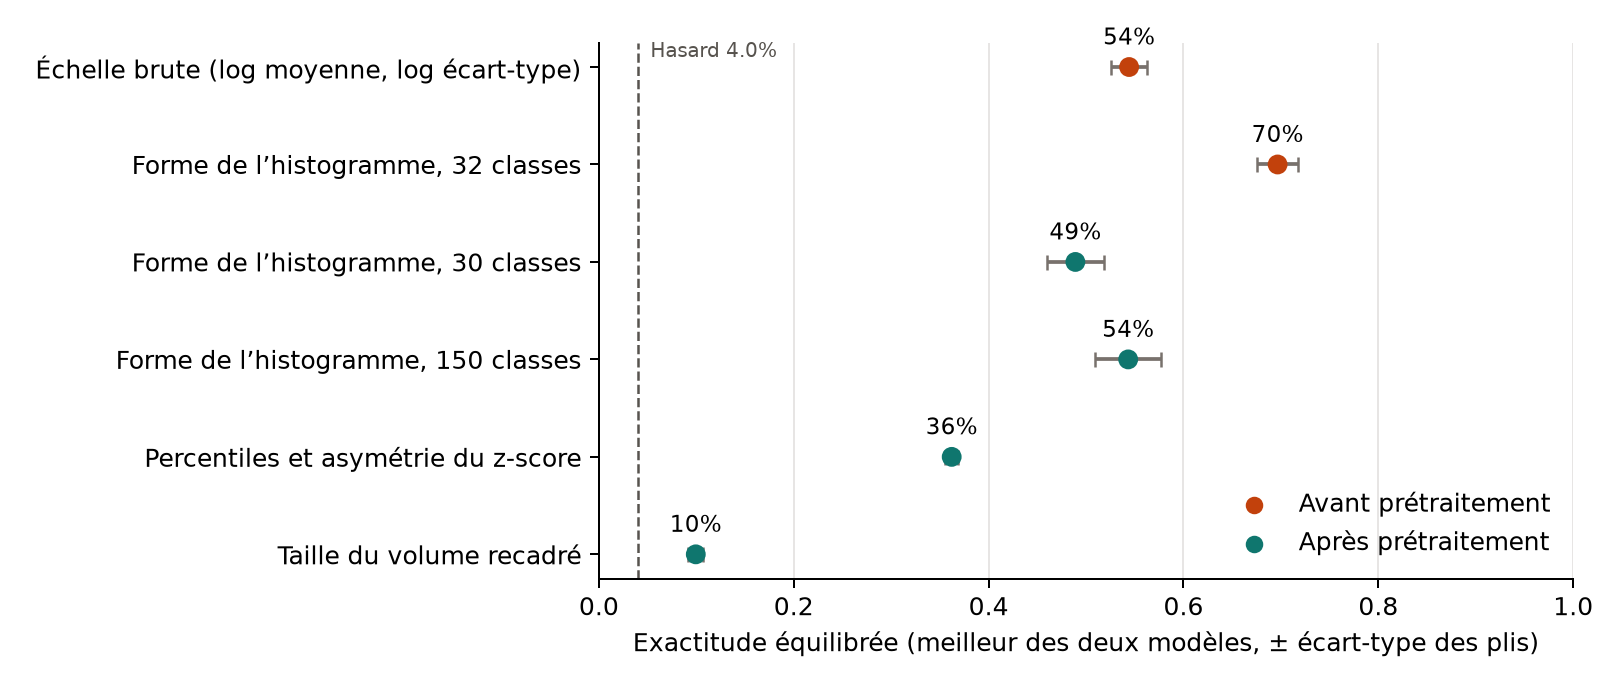
\includegraphics[width=\linewidth]{figures/s6_empreinte_centre.png}
  \caption{Empreinte du centre (S6) : exactitude équilibrée de la prédiction du centre selon la représentation, avant et après prétraitement (hasard : 4~\%).}
  \label{fig:yosra-s6}
\end{figure}

\section{Prédiction d'échec et effet du temps : protocole C1 préparé}
\label{sec:yosra-s7-s8}

S7 met en relation la distance au train du pli et l'erreur $1 - \mathrm{Dice}$ par centre.
Une validation leave-one-center-out produit des prédictions hors calibration.
La régression et le seuil d'alerte sont ajustés uniquement sur les autres centres de validation.
La différence de Dice par rapport au test ID est rapportée séparément.
Sans les résultats C3 de C1, ni corrélation empirique ni performance d'alerte ne peuvent être annoncées.

S8 compare les associations du centre et du délai post-AVC par modèles linéaires emboîtés sur les mêmes cas complets.
Le délai est transformé par $\log(1 + \textrm{jours})$.
Le test de permutation préserve le centre.
Les délais manquants, la sélection des cas et les confusions possibles limitent l'interprétation.
Le protocole n'établit pas une relation causale.

\section{Caractéristiques du réseau (C6 v2)}
\label{sec:yosra-c6}

La version C6 v2 mesure le décalage dans l'espace appris par le réseau plutôt que sur les
intensités. Le modèle C8 (U-Net 3D, augmentation d'intensité, pli 0) est gelé et utilisé en
mode évaluation, sans gradient et sans masque lésionnel. Pour chaque sujet, la sortie du
bottleneck, la couche que lit le classifieur de centre de DANN, est moyennée dans l'espace :
on obtient un vecteur de 320 valeurs par scan.
L'entrée est le volume C1 complet, complété par des zéros jusqu'à un multiple de 16. Le réseau
a été entraîné sur des patchs $96^3$ : sur le volume entier, les normalisations d'instance
portent sur une autre étendue. La même règle est appliquée à tous les scans, ce qui garde la
comparaison entre centres cohérente.

La comparaison d'empreinte baseline / augmentation / DANN demande les checkpoints baseline et
DANN du même protocole ; elle reste à faire.

\section{Démonstration et limites}
\label{sec:yosra-demo}

L'application Gradio affiche les coupes d'une IRM et un masque, calcule le volume lésionnel en mL et accepte une carte d'incertitude.
Un adaptateur permet de brancher le modèle final.
NiiVue fournit une vue 3D locale sur la route \texttt{/viewer/} du même serveur.
ANTsPy peut recaler un template MNI et transférer un atlas de labels ; une inspection visuelle demeure nécessaire avant de nommer les régions.

L'alerte individuelle d'intensité utilise un quantile de validation distinct du seuil par centre.
Elle n'est ni une garantie de performance ni une décision clinique.
En l'absence d'une entrée requise, l'application indique ce qui manque au lieu de créer un résultat.
Le support animé de secours est synthétique et explicitement étiqueté.

\subsection{Interface web du projet}
\label{sec:yosra-frontend}

Une application web (\texttt{frontend/}) présente l'ensemble du projet en dix pages :
vue d'ensemble, avancement du pipeline, contrôle qualité, prétraitement Spark, décalage entre
centres, modèles et Dice, adaptation de domaine, démonstration IRM avec vue 3D, conclusions
et galerie des figures. Le serveur FastAPI lit uniquement les rapports versionnés du dépôt
(\texttt{analysis/reports}, \texttt{preprocessing/reports}, \texttt{baselines/outputs},
\texttt{adaptation/outputs}, \texttt{integration/reports}) : aucun chiffre n'est simulé, et une
expérience absente est signalée comme telle. Chaque page et chaque carte indiquent qui a
produit le résultat. L'interface fonctionne sans étape de construction ni ressource externe ;
seules les figures des dossiers de résultats sont servies, jamais les données IRM. Sept tests
couvrent l'API (\texttt{frontend/tests/test\_server.py}).

\subsection{Branchement du modèle C8}
\label{sec:yosra-c8}

La démonstration (\texttt{demo/app.py}) et l'interface web appellent la fonction désignée par
la variable \texttt{AVC\_PREDICT\_ADAPTER}, au format \texttt{module:fonction}. L'adaptateur de
l'équipe, \texttt{adaptation.demo\_adapter:predict}, applique le prétraitement S4 puis le modèle
retenu (augmentation d'intensité, pli 0) et enregistre le masque en NIfTI \texttt{uint8} dans la
grille de l'IRM reçue. Il demande PyTorch et MONAI, absents de l'environnement de la
démonstration. Le pont \texttt{demo/c8\_bridge.py} lance donc cet adaptateur dans
l'environnement du modèle, dans un processus séparé, et récupère le masque ; la démonstration
utilise \texttt{AVC\_PREDICT\_ADAPTER=c8\_bridge:predict}. Le checkpoint est lu dans
\texttt{data/modeles/unet3d\_intensity\_pli0\_best.pt} (SHA-256 \texttt{ee6b93af\ldots abb6}),
hors du dépôt.

Sur le sujet OOD R034\_sub-r034s003\_ses-1, le rapport de la démonstration donne un volume
lésionnel de 27,058~mL (27\,058 voxels de 1~mm$^3$). Cette valeur concorde avec le volume
prédit lors de l'évaluation du modèle : 27,054~mL dans le fichier \texttt{resultats\_ood\_test.csv}
de la run intensité, conservé hors du dépôt. Sur le sujet OOD R031\_sub-r031s006\_ses-1, envoyé
sans masque à l'interface web, le modèle prédit 33,8~mL pour 27,7~mL annotés, soit un Dice de
0,745, en environ 35~s sur processeur. Ces deux cas vérifient le branchement ; ils ne constituent
pas une évaluation. Le modèle ne produit pas de carte d'incertitude. Cinq tests couvrent les
erreurs du pont (\texttt{tests/test\_c8\_bridge.py}).

\section{Discussion et travaux à terminer}
\label{sec:yosra-discussion}

Les principales limites actuelles sont la quarantaine QC à relire collectivement, le faible nombre de centres pour calibrer un prédicteur d'échec, la dépendance des distances aux effectifs, les métadonnées manquantes et l'absence locale des checkpoints et des Dice correspondant à C1 v2.
Les résultats RQ3 du pli 0 et le checkpoint C8 sont désormais disponibles (chapitre RQ3,
conclusion). Les analyses S7 et S8 sur C1 v2 attendent encore les Dice par sujet, y compris
sur la validation, qui sert à calibrer le seuil d'alerte sans consulter le test. L'empreinte
avant/après DANN attend les checkpoints baseline et DANN. La vidéo de vraie inférence et la
relecture collective restent à faire.
Une analyse S8 historique distincte est disponible plus bas (section~\ref{sec:yosra-s8-historique}).
Les références bibliographiques du document de projet doivent être vérifiées dans leurs publications originales avant d'être reprises dans la version remise.

\section{Compléments vérifiés de la livraison v2}
\label{sec:yosra-livraison}

L'export nnU-Net contient 916 images et labels d'entraînement, 499 images de test (231 ID, 268 OOD) et cinq plis (\nolinkurl{preprocessing/reports/export_v2.json}).
Le contrôle officiel nnU-Net reste à lancer dans l'environnement d'entraînement de Fayfa.
Les autres appartenances de v1 sont conservées.

L'analyse descriptive S8 trouve 1\,073 délais utilisables et 342 manquants ou invalides ; le délai médian est de 365 jours.
Huit centres n'ont aucun délai utilisable.
L'association centre / log-délai (eta carré 0,7475) souligne la nécessité de tenir compte du centre ; elle ne mesure pas l'effet du délai sur le Dice.
Voir \nolinkurl{analysis/reports/s8_metadata/} (\nolinkurl{summary.json}).

Le seuil individuel d'atypie du pli~0 vaut 0,114885 : référence de 733 scans du train, quantile 95~\% sur 183 scans de validation.
Aucun test ID/OOD n'a servi à ce réglage.
Le seuil est enregistré dans \texttt{data/demo/reference\_ood.json} (pli 0, quantile 0,95,
733 scans d'entraînement, 183 de validation), hors du dépôt comme l'ensemble de \texttt{data/}.

Chrome a chargé l'application, produit le rapport synthétique de 2,091~mL, puis affiché les coupes et le rendu 3D NiiVue sans erreur JavaScript (\nolinkurl{docs/pipeline/demo_verification/browser_report.json}).
L'image Docker a été construite et ses routes ainsi que le calcul du rapport ont été testés (\nolinkurl{docs/pipeline/verification.json}).
La vidéo de secours MP4 utilise ces captures réelles d'interface sur un phantom explicitement synthétique ; elle ne montre pas une inférence du réseau.

L'atlas Harvard-Oxford et le template compatible MNI152NLin6Asym ont été récupérés avec leurs sources et empreintes dans \nolinkurl{data/demo/atlas/provenance.json} (hors du dépôt ; copie versionnée : \nolinkurl{docs/pipeline/demo_verification/atlas_provenance.json}).
Les labels corticaux sont prioritaires, puis les labels sous-corticaux décalés de 100 ; les zones non couvertes gardent la valeur zéro.
Le recalage natif exige une relecture anatomique.
Sources : Nilearn Harvard-Oxford\footnote{\url{https://nilearn.github.io/stable/modules/generated/nilearn.datasets.fetch_atlas_harvard_oxford.html}} et TemplateFlow MNI152NLin6Asym\footnote{\url{https://github.com/templateflow/tpl-MNI152NLin6Asym}}.

Le recalage SyN sur l'exemple réel a été exécuté.
Atlas et IRM ont la même grille, les labels restent entiers et 97,75~\% des voxels atlas non nuls se trouvent dans le support d'intensité de l'image (\nolinkurl{docs/pipeline/verification.json}).
La planche locale \nolinkurl{data/demo/registration/qc_overlay.png} (hors du dépôt) a été examinée dans trois plans ; cela ne remplace pas une relecture anatomique experte.
Le rapport régional utilise le masque de référence fourni, sans inférence de réseau.

\section{S8 : résultat exploratoire sur les baselines récupérées}
\label{sec:yosra-s8-historique}

Le 12 novembre, les scores historiques de \texttt{cnn\_pretrained\_freeze-none} ont été rattachés à leur propre partition (903 train, 226 ID validation, 287 OOD), sans les reclasser dans C1 v2.
L'analyse utilise 167 cas ID complets de 31 centres et 257 cas OOD de 12 centres.
En ID, 58 délais manquent ou sont invalides et un Dice est absent ; en OOD, 30 délais manquent ou sont invalides.
Le Dice absent du cas à masque vide n'est pas remplacé par un score supposé.

Après ajustement sur le centre, l'ajout de $\log(1 + \textrm{délai})$ augmente le R$^2$ de 0,000046 en ID ($p$ exploratoire $= 0{,}911$) et de 0,03808 en OOD ($p = 0{,}001$ ; 999 permutations intra-centre pour chaque groupe).
Après ajout de $\log(1 + \textrm{volume lésionnel})$, ces gains sont respectivement 0,000711 et 0,000217 (\nolinkurl{analysis/reports/s8_historical/summary.json}).
L'association OOD dépend donc fortement des variables prises en compte ; elle ne permet pas d'attribuer un effet causal au temps.
Le volume est une analyse de sensibilité, pas un ajustement causal validé.
La figure~\ref{fig:yosra-s8} montre les cas utilisés.

\begin{figure}[htbp]
  \centering
  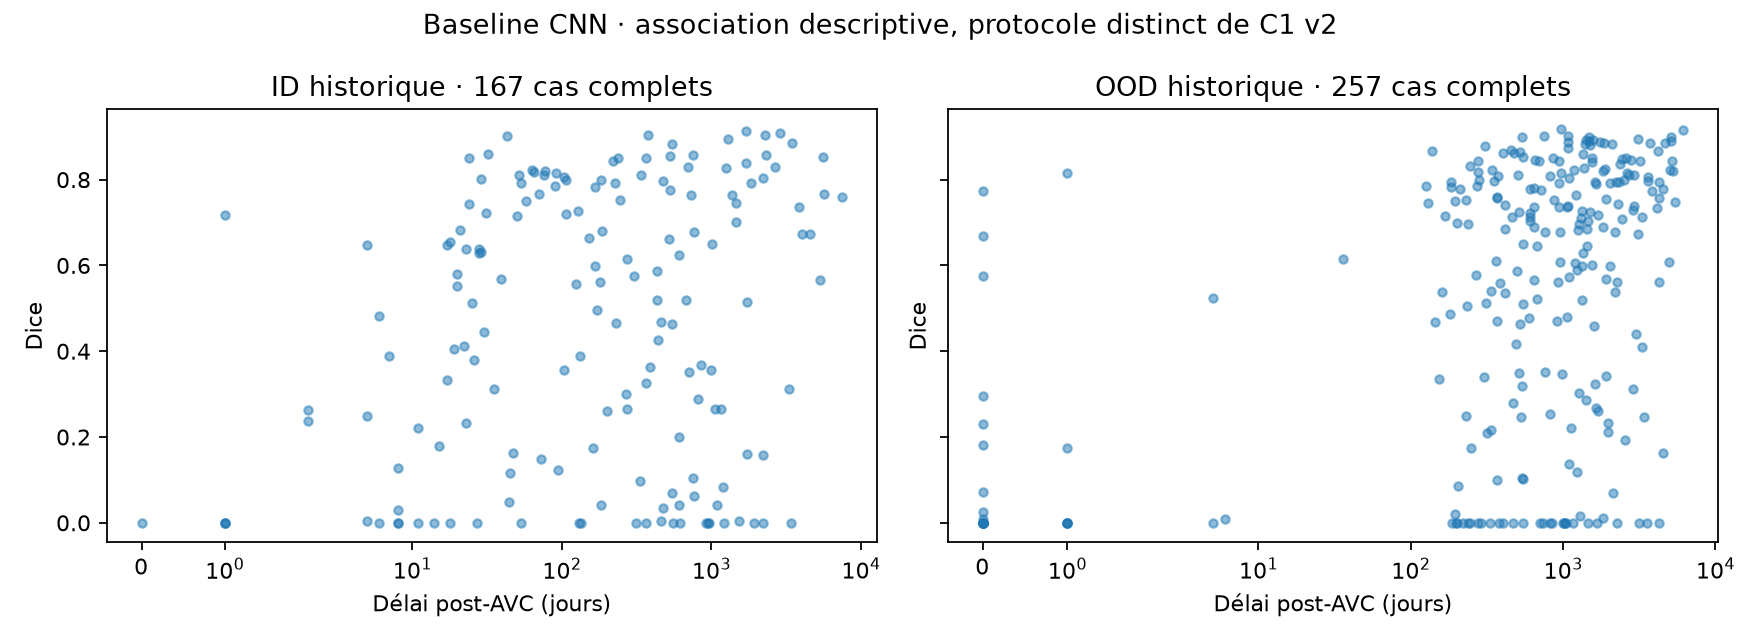
\includegraphics[width=\linewidth]{analysis/reports/s8_historical/time_dice.png}
  \caption{Dice de la baseline CNN historique selon le délai post-AVC, cas complets ID (167) et OOD (257) ; protocole distinct de C1 v2.}
  \label{fig:yosra-s8}
\end{figure}

Ces deux tests sont exploratoires, sans correction de multiplicité.
L'ID a participé au choix historique du modèle et n'est pas un test indépendant.
La partition et le prétraitement diffèrent de C1 v2.
Les résultats des autres baselines sont résumés séparément sur leurs effectifs disponibles, sans comparaison appariée implicite.

Livrables reproductibles : \nolinkurl{analysis/historical_baselines.py}, \nolinkurl{analysis/reports/s8_historical/summary.json}, \nolinkurl{README.md}, \nolinkurl{model_summary.csv}, \nolinkurl{missing_by_center.csv} et \nolinkurl{time_dice.png}.
Les empreintes des fichiers sources sont conservées.

\section{S6 : complément sur l'incertitude}
\label{sec:yosra-s6-incertitude}

Une évaluation complémentaire utilise 912 sujets d'entraînement et 228 sujets réservés, stratifiés parmi les mêmes 25 centres.
Deux classifieurs fixés, régression logistique et forêt aléatoire, sont évalués sur les mêmes sujets.
Les sujets réservés sont ensuite rééchantillonnés 10\,000 fois à l'intérieur de chaque centre, avec les mêmes indices pour toutes les représentations ; l'exactitude équilibrée donne le même poids aux centres.

Pour la forêt aléatoire, le score avant traitement (32 classes) est de 70,1~\%, avec un intervalle percentile conditionnel à 95~\% de [64,6 ; 75,5]~\%.
Après traitement (30 classes), il est de 51,1~\% [45,3 ; 57,0]~\%.
La différence appariée après moins avant est de $-19{,}0$ points [$-25{,}5$ ; $-12{,}6$].
Pour la régression logistique, elle est de $-21{,}5$ points [$-27{,}4$ ; $-15{,}5$] (\nolinkurl{analysis/reports/s6_uncertainty/intervals.csv}, \nolinkurl{analysis/reports/s6_uncertainty/paired_differences.csv}).
La variante après traitement à 150 classes est aussi rapportée pour montrer la sensibilité à la représentation, sans sélectionner uniquement le meilleur score.
La figure~\ref{fig:yosra-s6-incertitude} présente ces intervalles.

\begin{figure}[htbp]
  \centering
  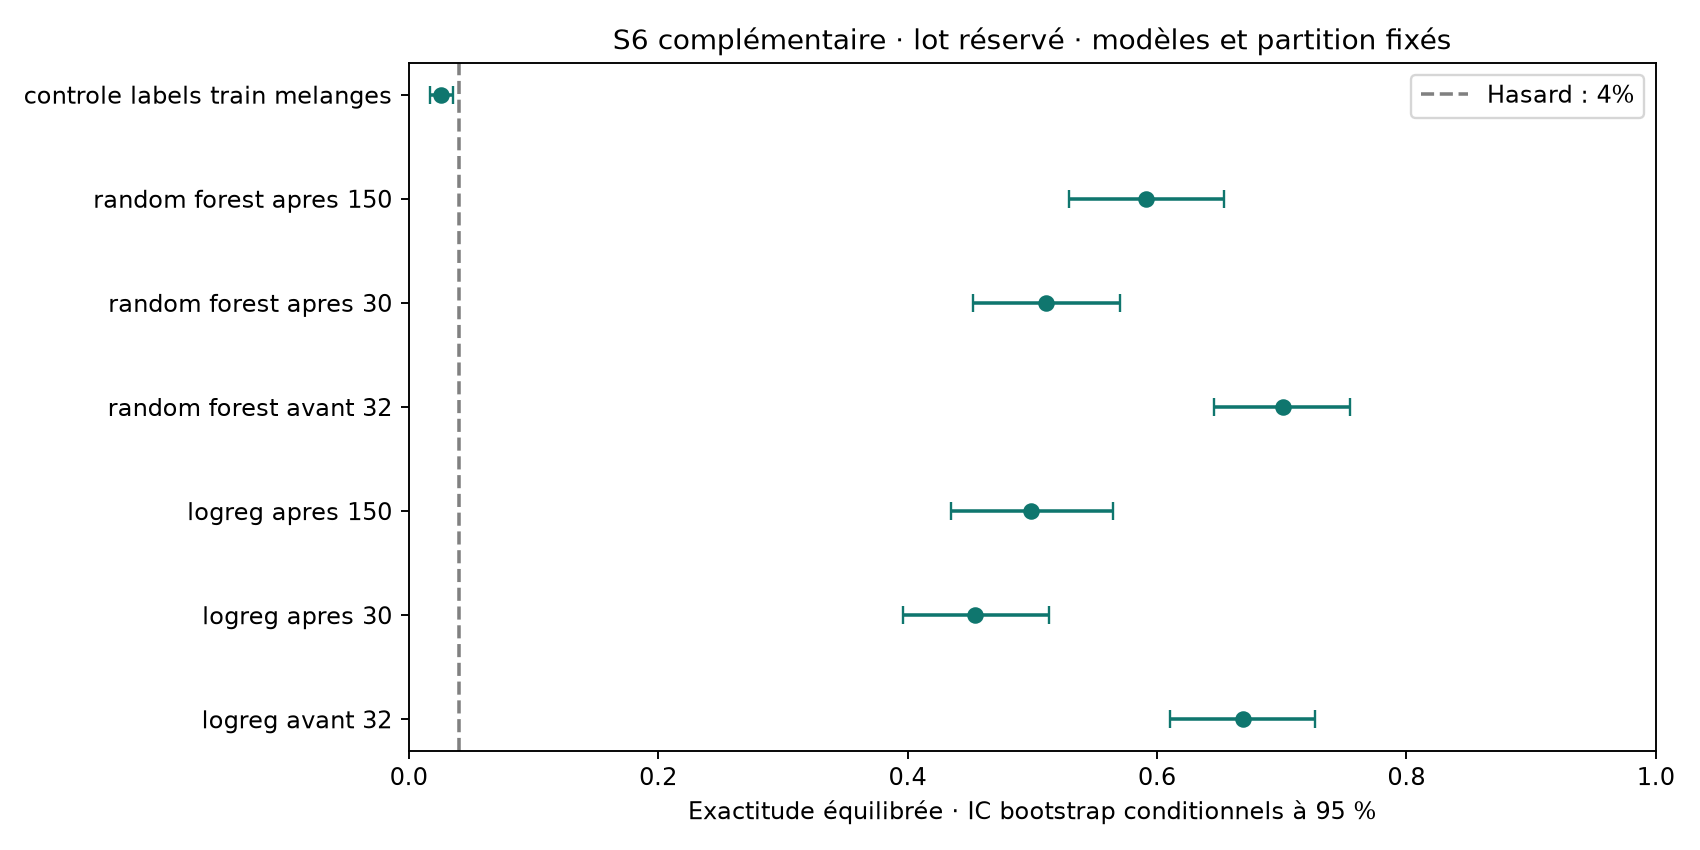
\includegraphics[width=\linewidth]{analysis/reports/s6_uncertainty/confidence_intervals.png}
  \caption{Exactitude équilibrée de la reconnaissance du centre sur le lot réservé, avec IC bootstrap conditionnels à 95~\% (modèles et partition fixés).}
  \label{fig:yosra-s6-incertitude}
\end{figure}

Ces intervalles conditionnent sur les modèles et la partition fixés : ils n'incluent pas la variabilité d'un nouvel entraînement.
La cohorte avait déjà été explorée en S6, et la granularité avant/après reste différente.
Il s'agit d'un complément exploratoire, pas d'une validation externe ni d'un effet causal isolé du prétraitement.
Les centres sont présents dans le train et le test : l'expérience mesure leur reconnaissance, pas la segmentation dans un centre inconnu.
Les moyennes des cinq plis précédentes restent inchangées et ne doivent pas être confondues avec ces nouveaux scores.

Livrables : \nolinkurl{analysis/reports/s6_uncertainty/README.md}, \nolinkurl{intervals.csv}, \nolinkurl{paired_differences.csv}, \nolinkurl{summary.json} et \nolinkurl{confidence_intervals.png}.
Les prédictions individuelles restent dans \nolinkurl{data/analysis/s6_uncertainty/} (hors du dépôt).

\section{Synthèse du contrôle qualité par centre}
\label{sec:yosra-qc}

La synthèse couvre les 1\,453 sujets inventoriés dans 55 centres.
Elle retrouve 1\,415 sujets retenus dans 54 centres, 38 exclus et aucune erreur active.
Les exclusions correspondent aux 37 cas R032 pour espacement non fiable et au cas R065 mis en quarantaine pour annotation hors du support et du recadrage.
Cette synthèse n'ajoute aucune exclusion et ne remplace pas la relecture collective des décisions.

Parmi les 1\,415 sujets retenus, cinq masques sont vides et conservés comme cas négatifs ; 1\,410 sont non vides et aucun statut de masque n'est inconnu.
Le délai post-AVC est disponible pour 1\,073 sujets ; 342 délais sont manquants ou invalides (24,2~\%).
Huit centres retenus n'ont aucun délai utilisable.
Le drapeau CHRONICITY est présent pour 296 sujets et non renseigné pour 1\,119 ; cette absence ne permet pas de déduire un stade clinique.
Deux sujets SOOP portent l'avertissement de fichier de métadonnées vide : cet avertissement de fichier ne recouvre pas toutes les valeurs de délai absentes.

Les effectifs d'exclusion utilisent tout l'inventaire ; les pourcentages de métadonnées utilisent seulement les sujets retenus de chaque centre.
Pour R032, sans sujet retenu, les taux sont non définis plutôt que nuls.
Les colonnes inconnues ne sont pas assimilées à des masques non vides.
Le tableau détaillé, la figure, les motifs d'exclusion et les avertissements sont disponibles dans \nolinkurl{analysis/reports/qc_by_center/} (\nolinkurl{summary.json}, \nolinkurl{qc_by_center.csv}, \nolinkurl{exclusion_reasons.csv}, \nolinkurl{metadata_warnings.csv}).
% La figure qc_by_center.png (55 centres sur trois panneaux) n'est pas insérée : à la largeur de la page, son texte
% ferait environ 3 pt. Elle reste disponible dans analysis/reports/qc_by_center/.
\section{Vérification de l'intégration}
\label{sec:yosra-verification}

Après la fusion des contributions de l'équipe dans \texttt{main}, 310 tests réussissent :
50 pour le pipeline et les analyses, 7 pour l'interface web, 224 pour la généralisation et
l'adaptation (dont des patchs C1 réels) et 29 pour la calibration. Quatorze tests
d'entraînement (\texttt{adaptation/tests/test\_train.py}, \texttt{test\_continual.py}) échouent
sur le Mac de vérification : \texttt{torch.amp.GradScaler} n'existe pas dans torch 2.2.2,
dernière version disponible pour macOS Intel. L'entraînement est exécuté sur Kaggle ;
l'inférence du checkpoint C8 est vérifiée localement
(\texttt{integration/reports/verification.json}).

\setlength{\emergencystretch}{0pt}

% Chapitre nnU-Net 3D (contribution d'Anas), à inclure dans docs/rapport/rapport.tex par \input.
% Traduction française fidèle de « Stroke lesion segmentation with nnU-Net 3D — final results » (18 novembre 2026) :
% mêmes chiffres, même plan, mêmes réserves. « Hospital » est rendu par « centre », comme dans les autres chapitres.
% Les notes de présentation ont été retirées ; le glossaire est en annexe (docs/rapport/annexe_glossaire.tex).
% Les figures de ce rapport ne sont pas dans le dépôt : emplacements [FIGURE À FOURNIR PAR ANAS].

\newcommand{\figureafournir}[1]{%
  \fbox{\parbox{0.9\linewidth}{\centering\vspace{1.5em}\textbf{[FIGURE À FOURNIR PAR ANAS : #1]}\vspace{1.5em}}}}

\chapter{Segmentation des lésions d'AVC avec nnU-Net 3D : résultats finaux}
\label{chap:anas}

\section{Résumé}
\label{sec:anas-resume}

Un nnU-Net 3D complet, entraîné pendant 8~heures sur un GPU Kaggle, atteint un \textbf{Dice de 0,61 sur de nouveaux patients de centres connus (ID) et de 0,66 sur des centres jamais vus (OOD)}, contre 0,47 / 0,53 pour notre CNN 2.5D précédent.

\begin{itemize}
  \item \textbf{Le 3D dépasse le 2.5D d'environ +0,13 de Dice}, pour toutes les tailles de lésion. Le plus grand gain concerne les lésions minuscules, de moins de 1~mL (0,20 $\rightarrow$ 0,47 en OOD).
  \item \textbf{Le réseau plus grand n'a pas aidé.} Le Residual Encoder U-Net (102~M de paramètres) obtient le même score que le U-Net simple (31~M) : 0,59 contre 0,61 en ID, 0,66 contre 0,66 en OOD. Chacune de ses époques est 1,6 fois plus lente ; dans les mêmes 8~heures, il a donc fait 94 époques au lieu de 152.
  \item \textbf{Pas de baisse sur les centres jamais vus.} L'OOD est même légèrement supérieur, parce que les centres OOD ont des lésions plus grandes, surtout chroniques, qui sont plus faciles. Dans chaque classe de taille de lésion, l'OOD est aussi $\geq$ ID.
  \item \textbf{Les deux modèles sont sous-entraînés, pas sur-entraînés.} Les pertes d'entraînement et de validation restent proches, et le Dice de validation montait encore à la fin. nnU-Net s'entraîne normalement pendant 1\,000 époques ; nous en avons fait 152.
  \item \textbf{Les cas difficiles sont les AVC aigus (< 7 jours) et les lésions minuscules} (< 1~mL) : Dice de 0,31 à 0,47. Seulement 6~\% des données sont aiguës, et la plupart viennent d'un seul centre, aux images de plus basse résolution.
\end{itemize}

\section{Données et découpage}
\label{sec:anas-donnees}

Nous utilisons \textbf{1\,416 IRM cérébrales pondérées en T1 provenant de 54 centres} (ATLAS v3 / ISLES'26), chacune avec un masque de lésion tracé par un expert.
Le centre R032 (37 IRM) a été retiré, car les en-têtes de ses fichiers sont incohérents.

Le découpage est fait \textbf{par centre}, ce qui permet de mesurer si le modèle fonctionne sur un centre qu'il n'a jamais vu (tableau~\ref{tab:anas-decoupage}).

\begin{table}[htbp]
  \centering
  \caption{Découpage par centre utilisé pour le CNN 2.5D, les baselines ML et nnU-Net 3D.}
  \label{tab:anas-decoupage}
  \small
  \begin{tabular}{lccl}
    \toprule
    Ensemble & Patients & Centres & Usage \\
    \midrule
    Entraînement & 903 & 40 & apprentissage des poids \\
    Validation ID & 226 & les mêmes 40 & \makecell[l]{choix du modèle, premiers contrôles\\(nouveaux patients, centres connus)} \\
    Test OOD & 287 & 14 autres & test final sur des centres jamais vus à l'entraînement \\
    \bottomrule
  \end{tabular}
\end{table}

Les 14 centres OOD ont été tirés au hasard (graine 0), avec au plus 60 patients chacun, pour qu'aucun grand centre ne forme à lui seul tout le jeu de test.
Le découpage ID est stratifié par centre.
Ce découpage est identique à celui utilisé pour le CNN 2.5D et les baselines ML : tous les chiffres de ce chapitre se comparent donc directement.

La lésion est minuscule par rapport au cerveau : environ \textbf{1~\% des voxels du cerveau}, médiane de 3,7~mL (ID) et de 5,6~mL (OOD).
C'est pourquoi nous mesurons le Dice (recouvrement) et non l'exactitude, qui vaudrait 99~\% pour un modèle qui ne prédit rien.

\section{Prétraitement}
\label{sec:anas-pretraitement}

Le prétraitement comporte deux parties : des corrections de données écrites par nous, puis le prétraitement automatique de nnU-Net, qui s'adapte au jeu de données.

\textbf{Nos corrections de données} (\nolinkurl{baselines/preprocessing/01_build_dataset.py}), identifiées pendant l'exploration des données :
\begin{enumerate}
  \item \textbf{Retrait du centre R032} : ses tailles de voxels sont incohérentes, et 2 IRM ne sont pas alignées avec leurs masques.
  \item \textbf{Nettoyage du fond de R029} : il valait une petite valeur non nulle au lieu de 0, ce qui fausse le recadrage du cerveau.
  \item \textbf{Masques strictement binaires} : 41 masques stockaient « 1 » sous la forme 0,99999998. Chaque masque est seuillé à 0,5 et enregistré avec l'en-tête exact de son T1, sans quoi le contrôle d'espacement de nnU-Net échoue.
  \item \textbf{Sous-échantillonnage de 105 IRM de très haute résolution} (centre SOOP, voxels de 0,25~mm, jusqu'à $1\,008 \times 1\,008 \times 348$) à 1~mm, avec anti-repliement. À pleine résolution, une IRM occupe 1,3~Go de mémoire.
  \item \textbf{Même orientation pour toutes les IRM} : toutes sont lues en orientation RAS (Right, Anterior, Superior).
\end{enumerate}

\textbf{Prétraitement automatique de nnU-Net} (\texttt{nnUNetv2\_plan\_and\_preprocess}) :
\begin{enumerate}
  \item \textbf{Empreinte} : nnU-Net mesure les tailles de voxels, les tailles d'image et les intensités du jeu de données, et en déduit ses réglages.
  \item \textbf{Recadrage} de chaque IRM sur le cerveau (la région non nulle).
  \item \textbf{Rééchantillonnage à $1 \times 1 \times 1$~mm} (l'espacement médian) : images par interpolation cubique, masques par interpolation linéaire puis seuillage.
  \item \textbf{Normalisation des intensités} par un z-score par IRM : (valeur $-$ moyenne) / écart-type. L'IRM n'a pas d'échelle d'intensité fixe ; cette étape ramène tous les scanners à la même échelle.
  \item \textbf{Planification du réseau} selon la mémoire du GPU : patches de $128 \times 128 \times 128$ voxels, lots de 2, 6 niveaux de résolution.
  \item \textbf{Enregistrement} des 1\,129 cas d'entraînement sous forme de tableaux compressés : 6,5~Go, 43 minutes sur le CPU de Kaggle.
\end{enumerate}

\textbf{Où cela a tourné.} L'ordinateur portable (GPU de 4~Go, 16~Go de RAM) est trop petit pour nnU-Net 3D : son prétraitement a été interrompu faute de mémoire.
Tout a tourné sur Kaggle, avec 2 GPU NVIDIA T4 (16~Go chacun) et des sessions gratuites de 12~h, pilotées depuis le portable par un script (\nolinkurl{kaggle/run.py}, hors du dépôt).
Le script envoie les données, lance les tâches, rapatrie les résultats et enregistre chaque run (paramètres, courbes, métriques, modèle) dans MLflow.

\section{Les deux modèles}
\label{sec:anas-modeles}

Les deux sont des U-Net 3D de même forme, planifiés par nnU-Net ; ils ne diffèrent que par le contenu de chaque niveau de l'encodeur.
Contrairement au CNN 2.5D, ils voient l'IRM en 3D (un cube de 12,8~cm à la fois) et utilisent donc le contexte au-dessus et au-dessous de chaque coupe.
La figure~\ref{fig:anas-architecture} résume les deux architectures.

\begin{figure}[htbp]
  \centering
  \figureafournir{schéma « Même forme en U pour les deux ; ResEnc met 3 fois plus de paramètres dans l'encodeur » (6 niveaux, de $128^3 \cdot 32$ à $4^3 \cdot 320$ caractéristiques ; U-Net simple 31~M, 152 époques en 8~h ; ResEnc U-Net 102~M, 94 époques en 8~h)}
  \caption{U-Net 3D planifié par nnU-Net pour nos données : 6 niveaux, la taille est divisée par deux à chaque niveau. Architecture tirée du \texttt{plans.json} de chaque run (hors du dépôt) ; nombres de paramètres tirés des checkpoints enregistrés.}
  \label{fig:anas-architecture}
\end{figure}

\begin{itemize}
  \item \textbf{Encodeur} (à gauche) : réduit l'image niveau par niveau et extrait des caractéristiques : d'abord des contours, puis des formes, puis « ceci ressemble à une lésion ».
  \item \textbf{Décodeur} (à droite) : agrandit à nouveau jusqu'à la taille d'origine et décide, voxel par voxel, lésion ou non. Les connexions de saut lui transmettent les détails fins que l'encodeur avait à chaque taille.
  \item \textbf{Blocs résiduels} (ResEnc) : chaque bloc ajoute son entrée à sa sortie, si bien que l'information et les gradients peuvent passer directement. Cela permet d'entraîner correctement un encodeur bien plus profond ; c'est l'idée de ResNet.
  \item \textbf{Commun aux deux} : normalisation d'instance et leaky ReLU après chaque convolution ; la sortie est une probabilité de lésion par voxel (softmax lésion / fond).
\end{itemize}

\section{Configuration de l'entraînement}
\label{sec:anas-entrainement}

Les deux modèles ont été entraînés avec la même recette nnU-Net, les mêmes données et le même \textbf{budget de 8~heures} ; seul le réseau diffère (tableau~\ref{tab:anas-config}).

\begin{table}[htbp]
  \centering
  \caption{Configuration d'entraînement commune aux deux modèles.}
  \label{tab:anas-config}
  \small
  \begin{tabular}{ll}
    \toprule
    Paramètre & Valeur \\
    \midrule
    Perte & \makecell[l]{perte Dice + entropie croisée, appliquée aussi à 4 résolutions\\plus basses (supervision profonde)} \\
    Optimiseur & SGD avec moment de Nesterov 0,99, décroissance des poids $3 \times 10^{-5}$ \\
    Taux d'apprentissage & \makecell[l]{part de 0,01 et décroît jusqu'à 0\\(polynomial : lr $\times$ (1 $-$ époque / dernière époque)$^{0,9}$)} \\
    Époque & 250 lots d'entraînement + 50 lots de validation \\
    Lot & \makecell[l]{2 patches de $128 \times 128 \times 128$ voxels ($12{,}8 \times 12{,}8 \times 12{,}8$~cm) ;\\1 patch sur 3 contient forcément de la lésion} \\
    Augmentation (à la volée) & \makecell[l]{rotation, mise à l'échelle, miroir, bruit et flou gaussiens,\\luminosité, contraste, gamma, basse résolution simulée} \\
    Précision & mixte (float16), pour tenir en mémoire et aller plus vite \\
    Modèle conservé & le checkpoint final (nnU-Net ne fait pas d'arrêt précoce) \\
    Inférence & \makecell[l]{fenêtre glissante sur toute l'IRM, sans augmentation miroir au test\\(environ 4 fois plus rapide)} \\
    \bottomrule
  \end{tabular}
\end{table}

\textbf{Le budget de temps.} nnU-Net s'entraîne normalement pendant 1\,000 époques, environ 2 jours sur une T4, mais une session Kaggle s'arrête au bout de 12~h.
Notre entraîneur mesure la durée d'une époque après 3 époques et réduit le nombre d'époques pour tenir en 8~h ; le taux d'apprentissage décroît ainsi quand même jusqu'à 0 selon le calendrier prévu (tableau~\ref{tab:anas-durees}).

\begin{table}[htbp]
  \centering
  \caption{Durées d'entraînement des deux modèles.}
  \label{tab:anas-durees}
  \small
  \begin{tabular}{lcc}
    \toprule
    & U-Net & ResEnc U-Net \\
    \midrule
    Durée par époque & 184~s & 301~s \\
    Époques en 8~h & 152 & 94 \\
    \makecell[l]{Session complète (installation + entraînement\\+ validation ID + prédiction OOD)} & 8~h~17~min & 8~h~22~min \\
    \bottomrule
  \end{tabular}
\end{table}

Les deux runs ont tourné en même temps, dans deux sessions Kaggle.
À la fin de chaque run, la validation ID (226 IRM) et la prédiction OOD (287 IRM) ont tourné en parallèle sur les deux GPU, en environ 10 minutes.

\section{Résultats}
\label{sec:anas-resultats}

Le U-Net 3D de 8~heures est le meilleur modèle : \textbf{Dice de 0,606 en ID et de 0,655 en OOD}, soit +0,13 par rapport au CNN 2.5D sur les deux ensembles (IC à 95~\% : +0,11 à +0,16).
Le test de 1,5~h montre que le gain vient du temps d'entraînement : avec seulement 26 époques, le même réseau ne faisait pas mieux que le CNN.
La figure~\ref{fig:anas-dice} compare les modèles.

\begin{figure}[htbp]
  \centering
  \figureafournir{« 8 h de nnU-Net 3D dépassent le CNN 2.5D de +0,13 de Dice ; le ResEnc plus grand n'apporte rien » : Dice moyen par patient avec intervalle bootstrap à 95~\%, mêmes patients pour chaque modèle (CNN 2.5D, U-Net 3D test de 1,5~h, U-Net 3D 8~h, ResEnc U-Net 3D 8~h ; ID 225 patients, OOD 287 patients)}
  \caption{Dice moyen par patient, avec intervalle bootstrap à 95~\%. Sources : métriques par cas de chaque run (\texttt{nnunet\_validation\_metrics\_cases.csv}, hors du dépôt ; CNN : \nolinkurl{baselines/outputs/fast_results/cnn_pretrained_freeze-none_cases.csv}) ; 225 patients ID et 287 patients OOD avec une lésion.}
  \label{fig:anas-dice}
\end{figure}

Le U-Net et le ResEnc sont statistiquement à égalité : ResEnc $-$ U-Net $= -0{,}015$ de Dice en ID (Wilcoxon $p = 0{,}62$) et $+0{,}001$ en OOD (IC à 95~\% : $-0{,}008$ à $+0{,}010$).
Chacun l'emporte sur environ la moitié des patients.
Le U-Net trouve un peu mieux les lésions (F1 par lésion de 0,60 contre 0,55 en ID) ; le ResEnc manque certaines lésions entièrement (voir les images plus bas).

Autres métriques du U-Net 8~h (ID / OOD) : distance de bord médiane HD95 de 9,5 / 5,4~mm, erreur de volume de 5,3 / 6,0~mL, F1 par lésion de 0,60 / 0,61.
Pour le CNN 2.5D, le F1 par lésion était de 0,34 / 0,33 : le modèle 3D trouve beaucoup plus de lésions séparées.

\subsection{Par taille de lésion}

La taille de la lésion est le facteur qui pèse le plus sur le Dice, pour tous les modèles.
Le modèle 3D aide surtout là où le CNN était le plus faible : les lésions minuscules, qu'un modèle 2D coupe par coupe manque facilement (figure~\ref{fig:anas-taille}).

\begin{figure}[htbp]
  \centering
  \figureafournir{« Le U-Net 3D gagne le plus sur les plus petites lésions : le Dice fait plus que doubler sous 1~mL » : Dice moyen par classe de taille de lésion, CNN 2.5D contre U-Net 3D 8~h, avec le gain (ID : $+0{,}26$, $+0{,}13$, $+0{,}07$, $+0{,}04$ ; OOD : $+0{,}27$, $+0{,}14$, $+0{,}07$, $+0{,}03$ pour $< 1$, 1--10, 10--50 et $> 50$~mL)}
  \caption{Dice moyen par classe de taille de lésion : CNN 2.5D (réglage fin complet) contre U-Net 3D 8~h. Taille de la lésion = volume de la lésion tracée par l'expert ; métriques par cas (hors du dépôt).}
  \label{fig:anas-taille}
\end{figure}

Le ResEnc U-Net reste à moins de 0,03 du U-Net dans chaque classe de taille.
À noter : OOD $\geq$ ID dans chaque classe ; le score OOD plus élevé n'est donc pas seulement dû à des lésions plus grandes, et rien n'indique de baisse sur les nouveaux centres.

\subsection{Par délai depuis l'AVC}

Les AVC aigus sont le point faible : à moins de 7 jours, le Dice vaut 0,43 en ID et 0,32 en OOD (tableau~\ref{tab:anas-delai}).

\begin{table}[htbp]
  \centering
  \caption{Dice du U-Net 8~h selon le stade de l'AVC (jours après l'AVC).}
  \label{tab:anas-delai}
  \small
  \begin{tabular}{lccc}
    \toprule
    Stade & Patients ID / OOD & Dice ID & Dice OOD \\
    \midrule
    aigu ($< 7$~j) & 12 / 26 & 0,43 & 0,32 \\
    subaigu (7--180~j) & 67 / 8 & 0,57 & 0,75 \\
    chronique ($> 180$~j) & 88 / 224 & 0,61 & 0,69 \\
    inconnu & 58 / 29 & 0,68 & 0,67 \\
    \bottomrule
  \end{tabular}
\end{table}

En IRM T1, une lésion aiguë est encore œdémateuse et à peine plus sombre que le tissu sain, alors qu'une lésion chronique est une cicatrice sombre et nette.
Les IRM aiguës sont aussi rares : 87 sur 1\,453 IRM de l'inventaire (6~\%).

\subsection{Par centre}

Le pire centre est \textbf{R049} (OOD, 24 patients, Dice 0,34).
C'est le cas extrême des points précédents : 23 de ses 24 patients sont aigus, ses lésions sont petites (médiane de 0,8~mL), et ses IRM ont une résolution plus basse (coupes de 1,5~mm, voxels de 3,4~mm\textsuperscript{3} au lieu de 1~mm\textsuperscript{3}).
En ID, \textbf{R009} (23 patients, Dice 0,41) a le même profil : lésions petites, en partie aiguës.
Les meilleurs centres d'au moins 3 patients atteignent un Dice de 0,77 à 0,88 (R003, R004, R057) ; ils ont surtout de grandes lésions chroniques.

\section{Ce que dessinent les modèles}
\label{sec:anas-exemples}

Chaque ligne correspond à un patient, montré sur la coupe axiale où la lésion de l'expert est la plus grande : l'IRM T1, le masque de l'expert, puis les masques tracés par le U-Net et par le ResEnc, avec le Dice de chacun sur toute l'IRM 3D.
Les patients ont été choisis pour montrer des réussites et des échecs typiques.
L'orientation des images est radiologique (la gauche du patient à droite).

\textbf{Là où cela fonctionne} (figure~\ref{fig:anas-reussites}).
\begin{itemize}
  \item \textbf{r003s005} (centre jamais vu, AVC chronique de 162~mL) : les deux modèles suivent la lésion presque exactement, Dice de 0,92 à 0,93. Les grandes lésions chroniques sont des cicatrices sombres et nettes en T1.
  \item \textbf{r058s059} (centre connu, 6~mL) : la lésion principale est trouvée par les deux. Les petites taches séparées du masque de l'expert sont en partie manquées, ce qui coûte du Dice (0,65 / 0,72).
  \item \textbf{r047s015} (centre jamais vu, 0,3~mL dans le tronc cérébral) : même cette lésion minuscule est trouvée par les deux, ce que le CNN 2.5D ne savait généralement pas faire.
\end{itemize}

\begin{figure}[htbp]
  \centering
  \figureafournir{exemples de réussite : r003s005 (R003, OOD, 162,0~mL ; Dice 0,92 / 0,93), r058s059 (R058, ID, 6,1~mL ; 0,65 / 0,72), r047s015 (R047, OOD, 0,3~mL ; 0,59 / 0,45) : IRM T1, masque de l'expert, U-Net, ResEnc U-Net}
  \caption{Réussites typiques : IRM T1, masque de l'expert, masques du U-Net et du ResEnc U-Net, avec leur Dice sur toute l'IRM 3D.}
  \label{fig:anas-reussites}
\end{figure}

\textbf{Là où cela échoue} (figure~\ref{fig:anas-echecs}).
\begin{itemize}
  \item \textbf{r009s040} (centre connu, 11~mL dans le cervelet) : le U-Net la trouve (0,60) ; le ResEnc la manque presque entièrement (0,02). Un exemple net de lésion entière manquée par le ResEnc.
  \item \textbf{r047s016} (centre jamais vu, 5~mL, deux lésions) : le U-Net trouve les deux (0,76) ; le ResEnc n'en marque que de petits morceaux (0,23). Les deux marquent aussi quelques petites taches que l'expert n'a pas tracées.
  \item \textbf{r049s010} (R049, aigu, 0,4~mL, IRM basse résolution) : les deux la manquent (Dice 0). Sur cette IRM floue, la lésion est à peine visible ; c'est l'échec typique du centre R049.
\end{itemize}

\begin{figure}[htbp]
  \centering
  \figureafournir{exemples d'échec : r009s040 (R009, ID, 10,6~mL ; Dice 0,60 / 0,02), r047s016 (R047, OOD, 5,4~mL ; 0,76 / 0,23), r049s010 (R049, OOD, 0,4~mL ; 0,00 / 0,00) : IRM T1, masque de l'expert, U-Net, ResEnc U-Net}
  \caption{Échecs typiques, présentés de la même façon.}
  \label{fig:anas-echecs}
\end{figure}

Tous les masques ont été vérifiés : recalculer le Dice à partir des fichiers de masques redonne exactement les valeurs des tableaux.

\section{Sous-apprentissage ou sur-apprentissage ?}
\label{sec:anas-apprentissage}

{\setlength{\emergencystretch}{2em}%
\textbf{Les deux modèles sont sous-entraînés (léger sous-apprentissage), pas sur-entraînés.}
Un sur-apprentissage se verrait par une perte de validation qui cesse de baisser puis remonte pendant que la perte d'entraînement continue de baisser.
Ici, les deux courbes baissent ensemble jusqu'à la fin (figure~\ref{fig:anas-pertes}).\par}

\begin{figure}[htbp]
  \centering
  \figureafournir{« Les pertes d'entraînement et de validation baissent ensemble : sous-entraîné, pas sur-entraîné » : perte nnU-Net (Dice + entropie croisée) selon les heures d'entraînement, moyenne glissante sur 9 époques, U-Net (152 époques, écart final 0,017) et ResEnc U-Net (94 époques, écart final 0,034)}
  \caption{Pertes d'entraînement et de validation. Sources : journaux d'entraînement nnU-Net (\texttt{training\_log\_*.txt}, hors du dépôt) des runs final-unet et final-resenc ; écart = moyenne des 10 dernières époques, validation moins entraînement.}
  \label{fig:anas-pertes}
\end{figure}

Trois signes vont dans le même sens :
\begin{itemize}
  \item \textbf{Écart faible.} À la fin, la perte de validation ne dépasse la perte d'entraînement que de 0,017 pour le U-Net, et de 0,034 pour le ResEnc. Le ResEnc, plus grand, commence à s'écarter un peu, ce qui est attendu avec 3 fois plus de paramètres.
  \item \textbf{Encore en progrès.} Le pseudo-Dice de validation du U-Net est passé de 0,73 (25~\% de l'entraînement) à 0,77 (50~\%), 0,79 (75~\%) et 0,81 (10 dernières époques). Il n'avait pas atteint de plateau.
  \item \textbf{Plus de temps a beaucoup aidé.} Le même U-Net est passé de 0,48 à 0,61 de Dice (ID) entre 26 époques (1,5~h) et 152 époques (8~h).
\end{itemize}

Le taux d'apprentissage décroît jusqu'à 0 à la fin de chaque run, par construction, ce qui aplatit aussi les courbes tout à la fin ; c'est la fin du calendrier, pas un plateau du modèle.
Le remède est donc d'\textbf{entraîner plus longtemps}, pas d'ajouter de la régularisation.

\section{Comment améliorer les modèles}
\label{sec:anas-ameliorations}

Les modèles sont limités par le \textbf{temps d'entraînement}, pas par la taille du modèle ; le premier levier est donc d'entraîner plus longtemps.
La liste est classée par gain attendu au regard du temps GPU qu'il coûte.
Les gains sont des estimations, non mesurées ici.

\begin{enumerate}
  \item \textbf{Entraîner le U-Net plus longtemps.} Reprendre depuis le checkpoint de 152 époques pour une ou deux sessions de 8~h de plus (le script prend déjà en charge \texttt{-{}-resume-from}). C'est le signal le plus net de nos courbes : le Dice de validation montait encore et il n'y a pas de sur-apprentissage.
  \item \textbf{Garder le U-Net simple, pas le ResEnc}, tant que le temps est limité. Le ResEnc n'a montré son avantage, dans l'étude des auteurs de nnU-Net, qu'avec le calendrier complet de 1\,000 époques. Avec 8~h, il est 3 fois plus grand, 1,6 fois plus lent, et pas meilleur.
  \item \textbf{Réactiver l'augmentation miroir au test} pour les prédictions finales. Elle ne coûte que du temps d'inférence (environ 40~min au lieu de 10), sans réentraînement, et apporte généralement un petit gain.
  \item \textbf{Travailler sur les AVC aigus et les lésions minuscules}, où le Dice est le plus bas (0,31 à 0,47). Pistes : échantillonner plus souvent les IRM aiguës et les petites lésions pendant l'entraînement, et évaluer à part les IRM basse résolution de R049. En T1 seul, un AVC aigu est à peine visible ; d'autres centres utilisent pour cela l'IRM de diffusion (DWI), que ce jeu de données ne contient pas.
  \item \textbf{Validation croisée à 5 plis et ensemble des 5 modèles} (le standard de nnU-Net). C'est plus fiable et généralement un peu meilleur, mais cela coûte 5 fois le temps GPU : environ 40~h, plus d'une semaine de quota Kaggle (30~h).
  \item \textbf{Tester le résultat OOD avec d'autres centres réservés} (validation croisée en laissant de côté des centres). Un seul découpage peut être chanceux ; plusieurs découpages confirmeraient qu'il n'y a pas de baisse sur les nouveaux centres.
\end{enumerate}

Quota GPU utilisé cette semaine : environ 19~h sur les 30~h disponibles sur Kaggle.

% Chapitre RQ3, à inclure dans le rapport (classe report) par % Chapitre RQ3, à inclure dans le rapport (classe report) par % Chapitre RQ3, à inclure dans le rapport (classe report) par \input{docs/rapport/chapitre_rq3}.
% Paquets attendus dans le préambule : babel (french), graphicx, booktabs, makecell, hyperref, float.
% Réglages à mettre dans le préambule du rapport final :
%   \addto\captionsfrench{\def\tablename{Tableau}}   % « Tableau » au lieu de « Table »
%   \hypersetup{hidelinks}                             % liens sans cadre rouge
% Les chemins des figures sont relatifs à la racine du dépôt.
% Citations : docs/rapport/references_rq3.bib, à ajouter à la commande \bibliography du rapport.

\chapter{Généralisation inter-centres (RQ3) et adaptation continue contrôlée}
\label{chap:rq3}

\section{Introduction}
\label{sec:rq3-introduction}

Ce chapitre étudie la robustesse d'un modèle de segmentation des lésions d'AVC face à des centres d'acquisition jamais vus.
La question de recherche RQ3 est la suivante : « Quelles techniques de data augmentation et/ou d'adaptation de domaine réduisent le plus efficacement l'écart de performance entre centres ? »
Nous mesurons cet écart entre des centres vus à l'entraînement (ID) et des centres non vus (OOD).
Nous décrivons d'abord le protocole et les techniques évaluées, puis les résultats et l'analyse des échecs.
Nous présentons ensuite une adaptation continue contrôlée, avant de discuter les limites de l'étude.

\section{Protocole expérimental}
\label{sec:rq3-protocole}

\paragraph{Données.}
Nous utilisons les images T1 d'ATLAS v2.0~\cite{liew2022atlas}, déjà débarrassées du crâne, après le prétraitement S4 de l'équipe : orientation RAS, rééchantillonnage à 1~mm, recadrage sur le cerveau et z-score dans le cerveau (\nolinkurl{preprocessing/week4.py}).
Le découpage est fixé dans \nolinkurl{splits.json}. Le centre R032 est exclu.

\paragraph{Découpage par centre.}
Six centres sont réservés au test OOD : R008, R028, R031, R034, R053 et SOOP.
Ils ont été choisis sur la taille des centres et la distance entre histogrammes d'intensité, sans consulter le Dice (champ \texttt{selection} de \nolinkurl{splits.json}).
Les autres centres sont répartis en cinq plis. Seul le pli~0 a été entraîné. Le tableau~\ref{tab:rq3-donnees} donne les effectifs.

\begin{table}[htbp]
  \centering
  \caption{Effectifs du pli~0.}
  \label{tab:rq3-donnees}
  \begin{tabular}{lrl}
    \toprule
    Ensemble & Sujets & Centres \\
    \midrule
    Entraînement & 733 & 39 \\
    Validation & 183 & 9 centres absents de l'entraînement \\
    Test ID & 185 & centres d'entraînement, sujets non vus \\
    Test OOD & 268 (265 à lésion non vide) & 6 \\
    \bottomrule
  \end{tabular}
\end{table}

Le découpage de \nolinkurl{splits.json} compte 184 sujets de validation.
L'un d'eux, le sujet r065s019 du centre R065, n'a pas de volume prétraité.
Le prétraitement S4 l'a rejeté, car une partie de sa lésion sort du recadrage calculé sur l'image.
Le chargeur l'écarte, et la validation porte donc sur 183 sujets, comme l'indiquent les journaux d'entraînement.
Un de ces 183 sujets a un masque vide : le Dice de validation est calculé sur 182 sujets.

\paragraph{Modèle et entraînement.}
Le réseau est un U-Net~3D de MONAI~\cite{cardoso2022monai} : canaux de 32 à 320, quatre sous-échantillonnages et deux unités résiduelles par niveau.
La normalisation d'instance est affine, ce qu'exige TENT.
L'entraînement utilise des patches de $96^3$ voxels, par lots de quatre patches (deux volumes $\times$ deux patches), dont la moitié est centrée sur la lésion.
Un miroir gauche-droite aléatoire est appliqué à toutes les runs.
La perte combine Dice et entropie croisée.
L'optimiseur AdamW part d'un taux d'apprentissage de $10^{-3}$, avec une décroissance polynomiale (puissance 0,9) et une décroissance des poids de $10^{-5}$.
La norme des gradients est écrêtée à 12.
Toutes les techniques reçoivent le même budget : 40\,000 itérations, graine 2026, calcul en fp32 sur un GPU T4.
Les runs ont été exécutées sur Kaggle (torch 2.11.0+cu130), sauf DANN.
DANN a été entraînée sur Google Colab (GPU T4, torch 2.14.1+cu130) jusqu'à l'itération 35\,889, puis reprise sur Kaggle jusqu'à 40\,000 (section~\ref{sec:rq3-limites}).

\paragraph{Sélection du modèle.}
Le modèle est validé toutes les 2\,000 itérations sur les 183 sujets de validation, en volume entier, par fenêtre glissante de $96^3$ (recouvrement 0,25).
Le checkpoint retenu est celui du meilleur Dice de validation. Il est évalué une seule fois sur les tests ID et OOD.

\paragraph{Métriques.}
Nous rapportons le Dice, la distance de Hausdorff à 95~\% (HD95), l'écart absolu de volume, le F1 des lésions et la différence du nombre de lésions.
Ces métriques sont communes à l'équipe (\nolinkurl{baselines/common.py}).
Le Dice n'est calculé que sur les sujets dont la lésion n'est pas vide.

\paragraph{Tests statistiques.}
Les moyennes sont données avec un intervalle de confiance (IC) à 95~\% par bootstrap percentile (10\,000 tirages).
Pour l'écart ID $-$ OOD, les deux groupes sont rééchantillonnés indépendamment.
Chaque technique est comparée à la baseline par un test des rangs signés de Wilcoxon~\cite{wilcoxon1945}, apparié sur les mêmes sujets.
Une correction de Holm~\cite{holm1979} est appliquée sur l'ensemble des techniques comparées.
La correction porte sur six comparaisons : intensité, BigAug, FDA, histogram matching, DANN et TENT.
BigAug et histogram matching sont aussi comparés directement à l'intensité (différence appariée, IC bootstrap, Wilcoxon), hors correction de Holm : ce sont des comparaisons secondaires avec la technique de référence.

\section{Techniques évaluées}
\label{sec:rq3-techniques}

Toutes les techniques partagent le réseau, les plis, les graines et le budget d'itérations. Seule l'étape propre à chaque technique change (\nolinkurl{adaptation/train.py}, \nolinkurl{generalization/configs/}).

\begin{itemize}
  \item \textbf{Augmentation d'intensité.} Gamma ($p = 0{,}3$) et contraste ($p = 0{,}3$), calibrés sur les seuls sujets d'entraînement ; bruit ($p = 0{,}2$), flou ($p = 0{,}2$), champ de biais ($p = 0{,}3$) et basse résolution ($p = 0{,}25$, jusqu'à 3~mm sur un axe).
  \item \textbf{BigAug}~\cite{zhang2020bigaug}. Flou, netteté, bruit, luminosité, gamma (plage calibrée) et transformation affine (échelle de 0,8 à 1,2, rotation de 20\textdegree), chacun avec $p = 0{,}5$. La déformation élastique est désactivée. Les plages sont adoucies par rapport à l'article pour préserver les petites lésions.
  \item \textbf{FDA} (Fourier Domain Adaptation)~\cite{yang2020fda}. L'amplitude basse fréquence est échangée avec celle d'une image d'un centre d'entraînement de référence (R059 pour le pli~0), avec $\beta$ entre 0,015 et 0,03 et $p = 0{,}5$.
  \item \textbf{DANN} (Domain-Adversarial Neural Network)~\cite{ganin2016dann}. Un classifieur des 39 centres d'entraînement est branché sur la sortie du goulot du réseau : moyenne spatiale, LayerNorm sans paramètres, puis perceptron de 64 unités. Une couche d'inversion du gradient le relie à l'encodeur. Le coefficient $\lambda$ est nul pendant les 2\,000 premières itérations, puis suit la montée proposée par Ganin et al.\ ($\gamma = 5$). La perte du centre a un poids de 0,1.
  \item \textbf{TENT}~\cite{wang2021tent}. Adaptation au test, sans étiquettes, du modèle baseline. Seuls les paramètres affines des normalisations sont modifiés, en minimisant l'entropie des prédictions, centre par centre (Adam, taux de $10^{-4}$, quatre patches par sujet).
  \item \textbf{Histogram matching.} L'histogramme d'intensité du cerveau de chaque volume est ramené vers un histogramme de référence, moyenné sur 20 sujets d'un centre d'entraînement (R059 pour le pli~0). La transformation est déterministe ($p = 1$) et s'applique aussi à la validation et au test. Faute de quota GPU, cette run a été lancée après les autres, avec une version ultérieure du code (section~\ref{sec:rq3-limites}).
\end{itemize}
Fan-Net~\cite{yu2023fannet} n'a pas été implémenté ; FDA en reprend le principe (échange d'amplitude de Fourier) sous une forme plus simple.

\section{Résultats RQ3}
\label{sec:rq3-resultats}

Le tableau~\ref{tab:rq3-resultats} résume les résultats sur 185 sujets ID et 265 sujets OOD (\nolinkurl{adaptation/outputs/rq3/tableau_rq3.md}).

\begin{table}[htbp]
  \centering
  \caption{Dice moyen par technique (pli~0), avec l'IC à 95~\% sous chaque valeur. $\Delta$ OOD : différence appariée à la baseline sur le test OOD ; $p$ : test de Wilcoxon, puis $p$ corrigé par Holm.}
  \label{tab:rq3-resultats}
  \small
  \setlength{\tabcolsep}{4pt}
  \begin{tabular}{lccccc}
    \toprule
    Technique & Dice ID & Dice OOD & \makecell{Écart\\ID $-$ OOD} & $\Delta$ OOD & $p$ OOD \\
    \midrule
    Baseline & \makecell{0,646\\{\footnotesize [0,611 ; 0,680]}} & \makecell{0,553\\{\footnotesize [0,517 ; 0,589]}} & \makecell{0,093\\{\footnotesize [0,044 ; 0,142]}} & -- & -- \\[2pt]
    Intensité & \makecell{0,656\\{\footnotesize [0,621 ; 0,690]}} & \makecell{0,577\\{\footnotesize [0,543 ; 0,611]}} & \makecell{0,080\\{\footnotesize [0,031 ; 0,126]}} & \makecell{+0,024\\{\footnotesize [0,008 ; 0,041]}} & \makecell{0,0014\\{\footnotesize (Holm 0,0068)}} \\[2pt]
    BigAug & \makecell{0,653\\{\footnotesize [0,619 ; 0,686]}} & \makecell{0,577\\{\footnotesize [0,543 ; 0,611]}} & \makecell{0,075\\{\footnotesize [0,028 ; 0,122]}} & \makecell{+0,025\\{\footnotesize [0,010 ; 0,040]}} & \makecell{0,035\\{\footnotesize (Holm 0,14)}} \\[2pt]
    FDA & \makecell{0,660\\{\footnotesize [0,626 ; 0,693]}} & \makecell{0,559\\{\footnotesize [0,524 ; 0,593]}} & \makecell{0,101\\{\footnotesize [0,053 ; 0,148]}} & \makecell{+0,006\\{\footnotesize [$-$0,007 ; 0,020]}} & \makecell{0,32\\{\footnotesize (Holm 0,49)}} \\[2pt]
    \makecell[l]{Histogram\\matching} & \makecell{0,646\\{\footnotesize [0,611 ; 0,681]}} & \makecell{0,570\\{\footnotesize [0,536 ; 0,604]}} & \makecell{0,077\\{\footnotesize [0,027 ; 0,125]}} & \makecell{+0,017\\{\footnotesize [0,001 ; 0,034]}} & \makecell{0,24\\{\footnotesize (Holm 0,49)}} \\[2pt]
    DANN & \makecell{0,650\\{\footnotesize [0,616 ; 0,684]}} & \makecell{0,549\\{\footnotesize [0,513 ; 0,584]}} & \makecell{0,102\\{\footnotesize [0,053 ; 0,150]}} & \makecell{$-$0,004\\{\footnotesize [$-$0,018 ; 0,009]}} & \makecell{0,13\\{\footnotesize (Holm 0,39)}} \\[2pt]
    \makecell[l]{Baseline\\+ TENT} & \makecell{0,645\\{\footnotesize [0,610 ; 0,679]}} & \makecell{0,542\\{\footnotesize [0,506 ; 0,578]}} & \makecell{0,104\\{\footnotesize [0,054 ; 0,153]}} & \makecell{$-$0,011\\{\footnotesize [$-$0,016 ; $-$0,006]}} & \makecell{$< 10^{-4}$\\{\footnotesize (Holm $< 10^{-4}$)}} \\[2pt]
    \bottomrule
  \end{tabular}
\end{table}

La figure~\ref{fig:rq3-dice-id-ood} montre les Dice ID et OOD de chaque technique avec leurs IC.
L'écart entre ID et OOD demeure pour toutes les techniques : il va de 0,075 à 0,104, et aucun IC ne contient 0.

\begin{figure}[htbp]
  \centering
  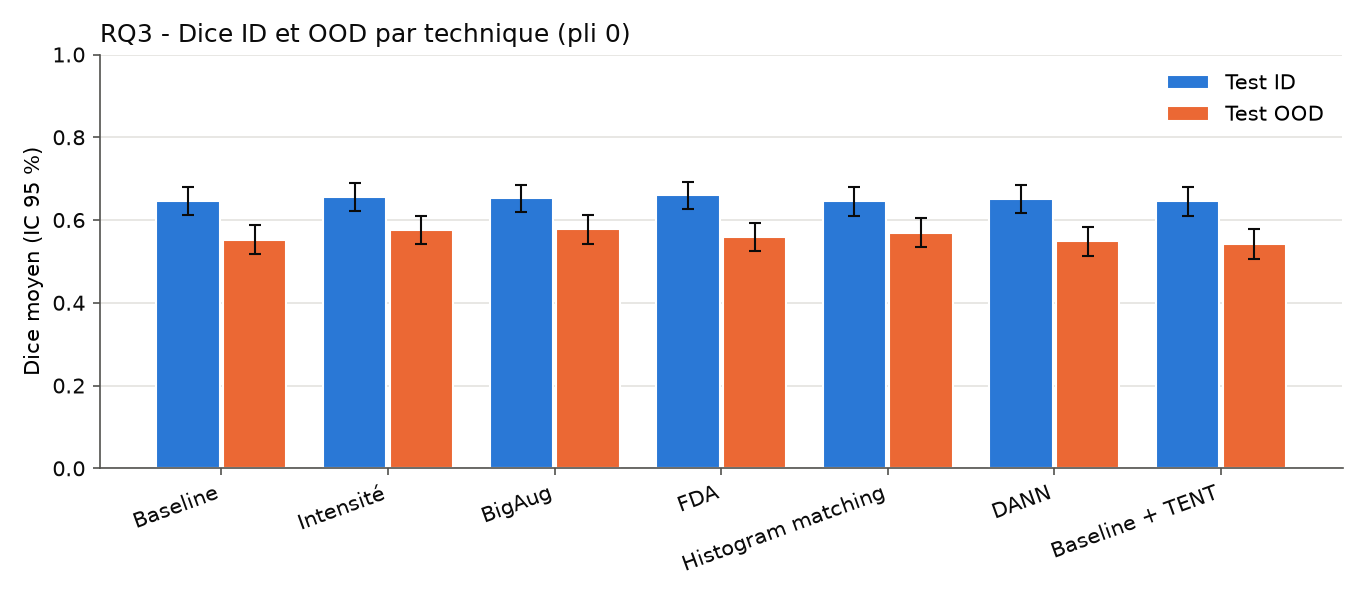
\includegraphics[width=0.8\linewidth]{figures/rq3/rq3_dice_id_ood.png}
  \caption{Dice moyen sur les tests ID et OOD par technique, avec IC à 95~\% (pli~0).}
  \label{fig:rq3-dice-id-ood}
\end{figure}

La figure~\ref{fig:rq3-delta-ood} montre la distribution des différences appariées à la baseline sur le test OOD.
\begin{itemize}
  \item L'augmentation d'intensité est la seule technique qui améliore le Dice OOD de façon significative après correction : $+0{,}024$ [0,008 ; 0,041], $p = 0{,}0014$, $p$ Holm $= 0{,}0068$. Le gain est réparti : 155 sujets sur 252 différences non nulles sont en sa faveur, pour une médiane de $+0{,}006$.
  \item BigAug obtient le même gain moyen ($+0{,}025$ [0,010 ; 0,040]), mais son Wilcoxon ($p = 0{,}035$) n'est plus significatif après correction ($p$ Holm $= 0{,}14$). La différence médiane avec la baseline est quasi nulle ($+0{,}001$ ; 135 sujets en sa faveur sur 250 différences non nulles), et la moyenne est tirée par quelques grands écarts, jusqu'à $+0{,}67$. C'est ce qui explique que le Wilcoxon, fondé sur les rangs, ne passe pas la correction de Holm. Son écart ID $-$ OOD est le plus faible (0,075), mais son IC chevauche celui de la baseline.
  \item FDA a le meilleur Dice ID (0,660), mais son gain sur la baseline n'est significatif après correction ni en ID (Wilcoxon $p = 0{,}012$, $p$ Holm $= 0{,}061$ ; $\Delta$ ID $= +0{,}014$ [$-$0,001 ; 0,029]), ni en OOD ($p = 0{,}32$).
  Avant correction, le Wilcoxon en ID est significatif alors que l'IC bootstrap de $\Delta$ ID contient 0, car les deux ne testent pas la même chose.
  Le Wilcoxon porte sur les rangs des différences appariées : 109 sujets sur 179 différences non nulles sont en faveur de FDA, pour une médiane de $+0{,}005$.
  L'IC porte sur la moyenne, que quelques grandes différences dans les deux sens (jusqu'à $-0{,}32$) rendent plus variable.
  \item Histogram matching améliore le Dice OOD en moyenne ($+0{,}017$ [0,001 ; 0,034]), mais pas de façon significative ($p = 0{,}24$, $p$ Holm $= 0{,}49$). L'IC bootstrap de $\Delta$ OOD exclut tout juste 0 alors que le Wilcoxon n'est pas significatif, pour la même raison que FDA en ID : l'IC porte sur la moyenne, tirée par quelques grands écarts (jusqu'à $+0{,}84$), et le Wilcoxon sur les rangs, avec une médiane nulle (125 sujets en sa faveur, 125 en sa défaveur). Son écart ID $-$ OOD (0,077) est proche de celui de BigAug.
  \item DANN ne se distingue de la baseline ni en ID ($p = 0{,}45$) ni en OOD ($p = 0{,}13$).
  \item TENT abaisse le Dice OOD de 0,011 [0,006 ; 0,016]. L'effet est petit mais systématique ($p < 10^{-4}$). En ID, la baisse est de 0,0007 [0,0002 ; 0,0012] ($p = 1{,}7 \times 10^{-4}$, $p$ Holm $= 1{,}0 \times 10^{-3}$).
\end{itemize}

\begin{figure}[htbp]
  \centering
  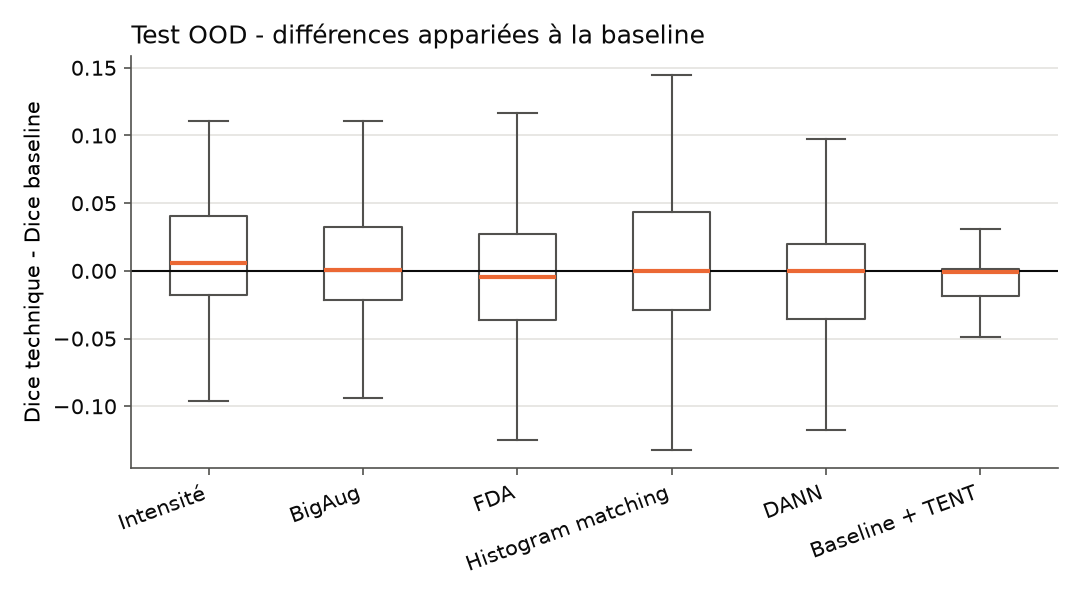
\includegraphics[width=0.8\linewidth]{figures/rq3/rq3_delta_ood.png}
  \caption{Différences appariées de Dice avec la baseline, par sujet, sur le test OOD.}
  \label{fig:rq3-delta-ood}
\end{figure}

\paragraph{BigAug et intensité.}
Le tableau~\ref{tab:rq3-bigaug-intensite} compare directement les deux techniques sur les mêmes sujets (\nolinkurl{adaptation/outputs/rq3/comparaisons.csv}).
Sur le test OOD, la différence moyenne BigAug $-$ intensité vaut $+0{,}001$ [$-0{,}010$ ; 0,012] ($p = 0{,}53$ ; 123 sujets en faveur de BigAug, 128 en faveur de l'intensité).
Sur le test ID, elle vaut $-0{,}003$ [$-0{,}017$ ; 0,011] ($p = 0{,}35$).
Aucun centre OOD ne les sépare : les différences vont de $-0{,}011$ (R034) à $+0{,}006$ (R008), toutes avec $p \geq 0{,}32$.
Les deux techniques sont donc équivalentes en Dice à la précision de cette étude.
Elles diffèrent sur deux points secondaires.
L'entraînement de BigAug dure 8,1~h contre 5,0~h pour l'intensité (\nolinkurl{adaptation/outputs/rq3/entrainement.csv}).
Le F1 des lésions OOD est plus élevé avec l'intensité qu'avec BigAug (0,450 contre 0,420), mais les deux restent sous la baseline (0,477, tableau~\ref{tab:rq3-secondaires}) : ce n'est qu'un avantage relatif face à BigAug.

\begin{table}[htbp]
  \centering
  \caption{Comparaison directe BigAug $-$ intensité par centre OOD (sujets appariés). Source : \texttt{comparaisons\_par\_centre.csv}.}
  \label{tab:rq3-bigaug-intensite}
  \small
  \setlength{\tabcolsep}{4pt}
  \begin{tabular}{lcccccc}
    \toprule
    Centre & n & Dice BigAug & Dice intensité & $\Delta$ moyen & \makecell{Sujets\\BigAug > / < intensité} & $p$ Wilcoxon \\
    \midrule
    R008 & 7 & 0,006 & 0,000 & +0,006 & 1 / 0 & 1 \\
    R028 & 26 & 0,652 & 0,649 & +0,003 & 16 / 10 & 0,50 \\
    R031 & 37 & 0,663 & 0,672 & $-$0,009 & 15 / 22 & 0,32 \\
    R034 & 24 & 0,642 & 0,653 & $-$0,011 & 11 / 12 & 0,76 \\
    R053 & 4 & 0,195 & 0,197 & $-$0,002 & 1 / 1 & 1 \\
    SOOP & 167 & 0,571 & 0,567 & +0,004 & 79 / 83 & 0,60 \\
    \midrule
    Total OOD & 265 & 0,577 & 0,577 & +0,001 & 123 / 128 & 0,53 \\
    \bottomrule
  \end{tabular}
\end{table}

\paragraph{Histogram matching et intensité.}
Le tableau~\ref{tab:rq3-hm-intensite} compare de la même façon histogram matching et intensité.
Sur le test OOD, la différence moyenne histogram matching $-$ intensité vaut $-0{,}007$ [$-0{,}023$ ; 0,009] ($p = 0{,}062$ ; 110 sujets en faveur d'histogram matching, 142 en faveur de l'intensité).
Sur le test ID, elle vaut $-0{,}010$ [$-0{,}025$ ; 0,005] ($p = 0{,}35$).
Le seul écart net par centre concerne R031 : $-0{,}059$ ($p = 0{,}0018$ ; 10 sujets contre 27), qui reste sous 0,05 après une correction de Bonferroni sur les six centres.
Histogram matching a en revanche un F1 des lésions OOD supérieur à celui de la baseline (0,486 contre 0,477) et le plus faible écart absolu de volume de toutes les techniques (9,1~ml, tableau~\ref{tab:rq3-secondaires}).

\begin{table}[htbp]
  \centering
  \caption{Comparaison directe histogram matching $-$ intensité par centre OOD (sujets appariés). HM : histogram matching. Source : \texttt{comparaisons\_par\_centre.csv}.}
  \label{tab:rq3-hm-intensite}
  \small
  \setlength{\tabcolsep}{4pt}
  \begin{tabular}{lcccccc}
    \toprule
    Centre & n & Dice HM & Dice intensité & $\Delta$ moyen & \makecell{Sujets\\HM > / < intensité} & $p$ Wilcoxon \\
    \midrule
    R008 & 7 & 0,019 & 0,000 & +0,019 & 1 / 0 & 1 \\
    R028 & 26 & 0,659 & 0,649 & +0,010 & 16 / 9 & 0,23 \\
    R031 & 37 & 0,614 & 0,672 & $-$0,059 & 10 / 27 & 0,0018 \\
    R034 & 24 & 0,648 & 0,653 & $-$0,005 & 14 / 9 & 0,41 \\
    R053 & 4 & 0,237 & 0,197 & +0,040 & 1 / 1 & 1 \\
    SOOP & 167 & 0,566 & 0,567 & 0,000 & 68 / 96 & 0,11 \\
    \midrule
    Total OOD & 265 & 0,570 & 0,577 & $-$0,007 & 110 / 142 & 0,062 \\
    \bottomrule
  \end{tabular}
\end{table}

\paragraph{Lecture des résultats négatifs.}
Les résultats de DANN et de TENT ne sont pas des défaillances techniques. La run DANN est allée à son terme, avec un contrôle de reprise validé (section~\ref{sec:rq3-limites}). TENT a été appliqué au modèle baseline sur les mêmes sujets. Les deux sont évalués comme les autres techniques.
Pour DANN, l'alignement des caractéristiques entre 39 centres n'apporte rien de mesurable.
Une explication compatible avec nos données est que les échecs OOD dépendent surtout de la taille et du contraste des lésions (section~\ref{sec:rq3-echecs}), deux facteurs que l'alignement des centres ne traite pas.
Pour TENT, la minimisation de l'entropie rend les prédictions plus tranchées sans étiquettes. La baisse touche surtout les lésions de plus de 50~ml (0,71 contre 0,74, tableau~\ref{tab:rq3-taille}).

\paragraph{Métriques secondaires.}
Elles ne suivent pas toujours le Dice (tableau~\ref{tab:rq3-secondaires}).
Le F1 des lésions OOD baisse avec l'intensité (0,450 contre 0,477), BigAug (0,420), FDA et DANN (0,366 et 0,367) ; il augmente avec histogram matching (0,486) et TENT (0,495).
L'écart absolu de volume baisse surtout avec histogram matching (9,1~ml contre 11,1~ml), puis avec l'intensité (10,0~ml) et BigAug (10,9~ml).

\begin{table}[htbp]
  \centering
  \caption{Métriques secondaires moyennes sur le test OOD (\texttt{tableau\_rq3.csv}).}
  \label{tab:rq3-secondaires}
  \begin{tabular}{lccc}
    \toprule
    Technique & F1 des lésions & HD95 (mm) & Écart absolu de volume (ml) \\
    \midrule
    Baseline & 0,477 & 24,9 & 11,1 \\
    Intensité & 0,450 & 25,5 & 10,0 \\
    BigAug & 0,420 & 25,4 & 10,9 \\
    FDA & 0,366 & 26,1 & 13,3 \\
    Histogram matching & 0,486 & 24,9 & 9,1 \\
    DANN & 0,367 & 27,2 & 12,1 \\
    Baseline + TENT & 0,495 & 25,9 & 12,1 \\
    \bottomrule
  \end{tabular}
\end{table}

\paragraph{Validation et test.}
Les meilleurs Dice de validation vont de 0,427 à 0,443 (\nolinkurl{adaptation/outputs/rq3/entrainement.csv}). La validation ne départage donc pas les techniques.
Le Dice de validation (environ 0,43) est plus bas que celui du test ID (0,646) pour deux raisons.
La validation porte sur neuf centres non vus.
Ses lésions sont aussi plus petites : médiane de 1,26~ml et 43~\% sous 1~ml, contre 7,56~ml et 18~\% au test ID (volumes \texttt{lesion\_ml} des fichiers \texttt{qc.json}).

\section{Analyse des échecs}
\label{sec:rq3-echecs}

Les tableaux détaillés de cette section sont produits par le script \nolinkurl{adaptation/analyse_echecs.py}.
Ils se trouvent dans le dossier \nolinkurl{adaptation/outputs/rq3/echecs/}.

\subsection{Dice par centre OOD}

Le tableau~\ref{tab:rq3-centres} et la figure~\ref{fig:rq3-dice-centre} donnent le Dice moyen par centre.
Le contraste T1 est la différence entre le z-score moyen de la lésion et celui d'un anneau de 1 à 4~mm autour d'elle. Une lésion chronique est hypo-intense, et son contraste est négatif.

\begin{table}[htbp]
  \centering
  \caption{Centres OOD, rangés par distance décroissante au reste des centres. Vol. : volume médian des lésions ; J : jours après l'AVC (médiane) ; W1 : distance de Wasserstein ; Base. : baseline ; Int. : intensité ; HM : histogram matching ; TENT : baseline + TENT. Source : \texttt{par\_centre\_ood.csv}.}
  \label{tab:rq3-centres}
  \small
  \setlength{\tabcolsep}{3pt}
  \begin{tabular}{lcccccccccccc}
    \toprule
    & & & & & & \multicolumn{7}{c}{Dice moyen} \\
    \cmidrule(lr){7-13}
    Centre & \makecell{Sujets\\(lésion)} & \makecell{Vol.\\(ml)} & J & W1 & Contraste & Base. & Int. & BigAug & FDA & HM & DANN & TENT \\
    \midrule
    R008 & 7 (7) & 0,95 & 1 & 0,216 & $-$0,17 & 0,00 & 0,00 & 0,01 & 0,00 & 0,02 & 0,00 & 0,00 \\
    R031 & 37 (37) & 6,74 & 138 & 0,164 & $-$0,98 & 0,62 & 0,67 & 0,66 & 0,65 & 0,61 & 0,63 & 0,62 \\
    R028 & 26 (26) & 4,94 & 576 & 0,157 & $-$0,82 & 0,66 & 0,65 & 0,65 & 0,64 & 0,66 & 0,65 & 0,66 \\
    SOOP & 169 (167) & 22,75 & -- & 0,023 & $-$0,69 & 0,54 & 0,57 & 0,57 & 0,54 & 0,57 & 0,53 & 0,52 \\
    R053 & 5 (4) & 0,81 & 25 & 0,020 & $-$0,50 & 0,20 & 0,20 & 0,20 & 0,22 & 0,24 & 0,25 & 0,20 \\
    R034 & 24 (24) & 2,38 & 1\,506 & 0,014 & $-$0,64 & 0,63 & 0,65 & 0,64 & 0,66 & 0,65 & 0,64 & 0,63 \\
    \bottomrule
  \end{tabular}
\end{table}

\begin{figure}[htbp]
  \centering
  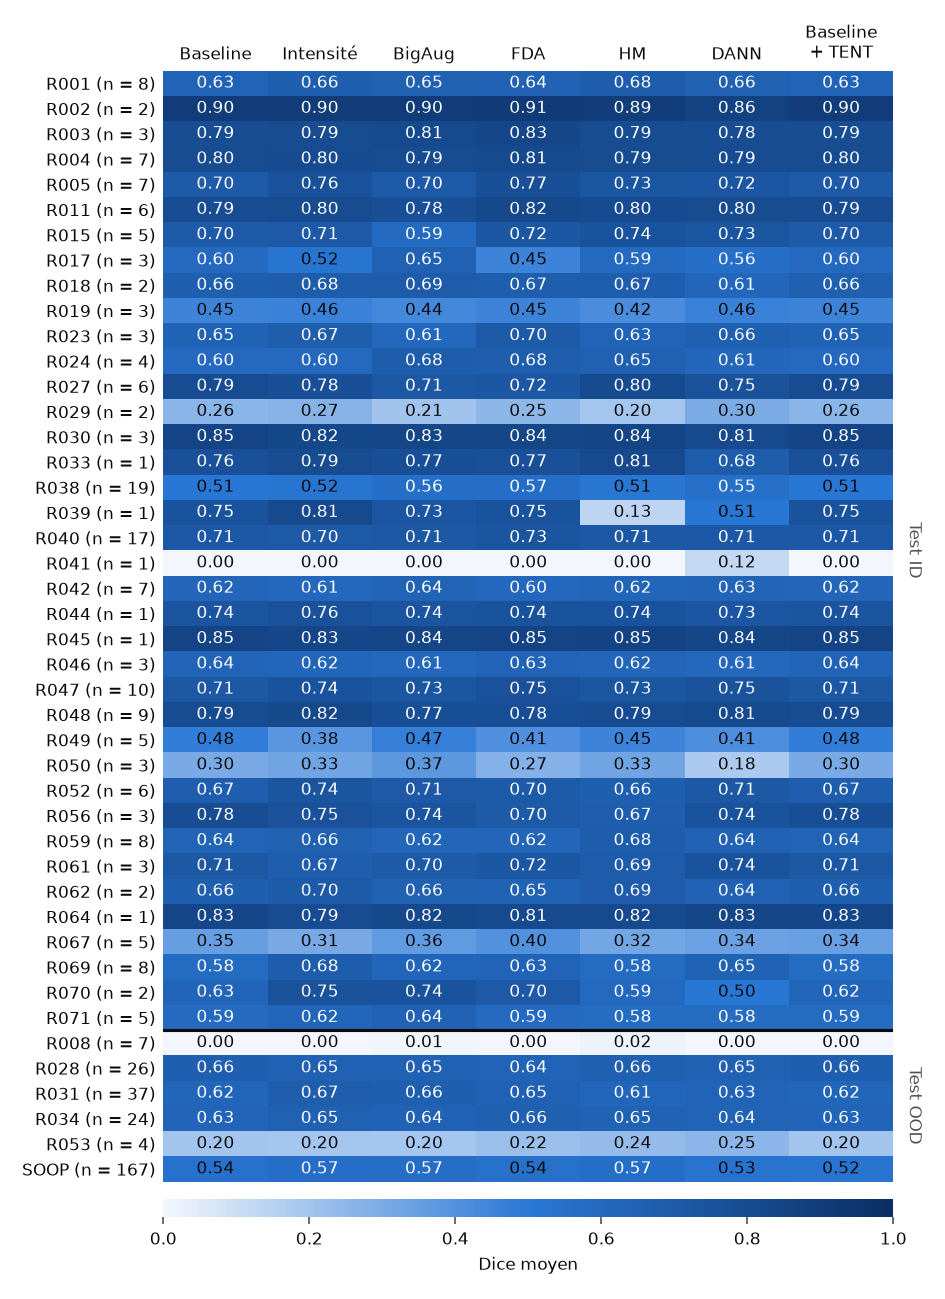
\includegraphics[width=\linewidth]{figures/rq3/rq3_dice_par_centre.png}
  \caption{Dice moyen par centre de test (ID et OOD) et par technique. HM : histogram matching.}
  \label{fig:rq3-dice-centre}
\end{figure}

\subsection{Taille des lésions}

La taille est le facteur le plus net.
Sur les 265 sujets OOD, la corrélation de Spearman entre le volume de la lésion et le Dice (modèle intensité) vaut $\rho = 0{,}53$ ($p < 10^{-4}$).
Le tableau~\ref{tab:rq3-taille} et la figure~\ref{fig:rq3-dice-taille} montrent que toutes les techniques suivent le même profil.
L'intensité gagne surtout entre 1 et 50~ml (0,50 et 0,67 contre 0,46 et 0,64 pour la baseline). BigAug gagne surtout au-dessus de 10~ml (0,68 et 0,77 contre 0,64 et 0,74).

\begin{table}[htbp]
  \centering
  \caption{Dice moyen par volume de lésion sur le test OOD (Dice ID entre parenthèses). L'adaptation continue porte sur un sous-ensemble des sujets.}
  \label{tab:rq3-taille}
  \small
  \begin{tabular}{lcccc}
    \toprule
    Technique & $< 1$~ml & 1--10~ml & 10--50~ml & $\geq 50$~ml \\
    \midrule
    Sujets OOD (ID) & 41 (34) & 86 (65) & 80 (48) & 58 (38) \\
    \midrule
    Baseline & 0,31 (0,48) & 0,46 (0,58) & 0,64 (0,71) & 0,74 (0,83) \\
    Intensité & 0,33 (0,46) & 0,50 (0,59) & 0,67 (0,74) & 0,74 (0,83) \\
    BigAug & 0,32 (0,43) & 0,48 (0,59) & 0,68 (0,75) & 0,77 (0,83) \\
    FDA & 0,30 (0,44) & 0,46 (0,61) & 0,66 (0,74) & 0,75 (0,84) \\
    Histogram matching & 0,33 (0,49) & 0,49 (0,58) & 0,66 (0,71) & 0,74 (0,83) \\
    DANN & 0,29 (0,46) & 0,45 (0,58) & 0,63 (0,73) & 0,75 (0,83) \\
    Baseline + TENT & 0,32 (0,48) & 0,46 (0,58) & 0,62 (0,71) & 0,71 (0,82) \\
    Continue (contrôlée) & 0,35 & 0,48 & 0,60 & 0,81 \\
    \bottomrule
  \end{tabular}
\end{table}

\begin{figure}[htbp]
  \centering
  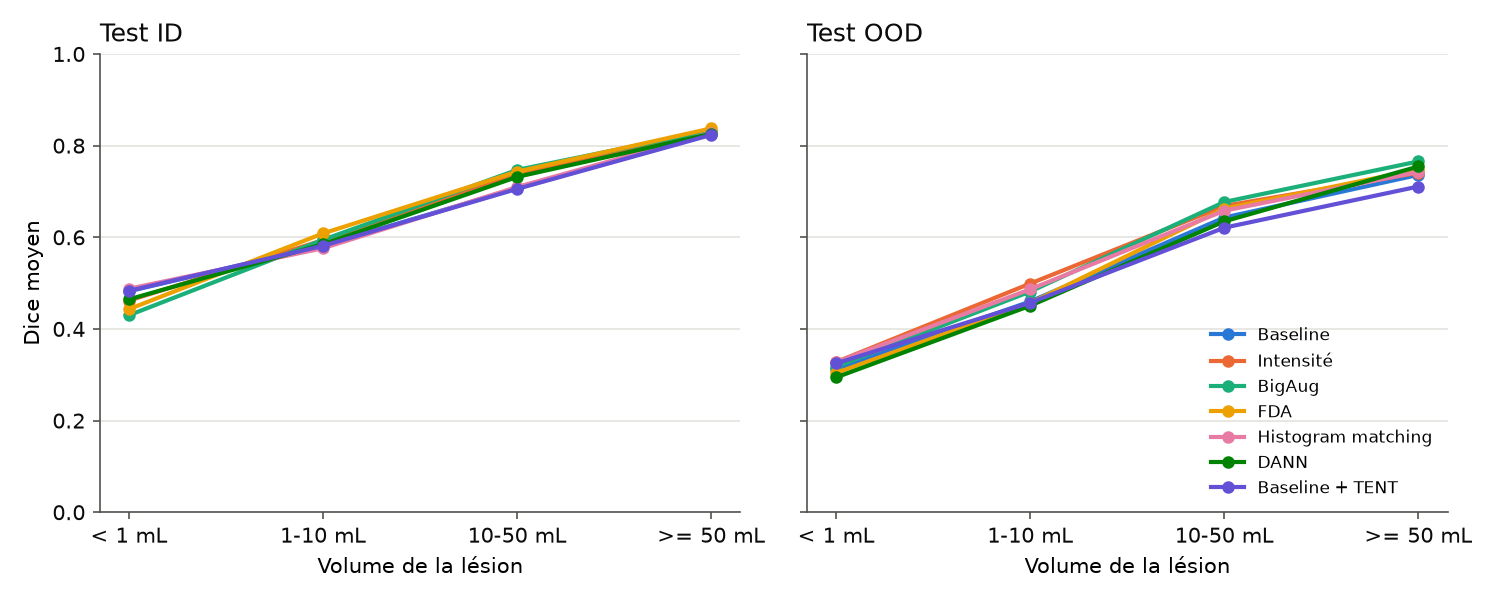
\includegraphics[width=\linewidth]{figures/rq3/rq3_dice_par_taille.png}
  \caption{Dice moyen par classe de volume de lésion, sur les tests ID (à gauche) et OOD (à droite).}
  \label{fig:rq3-dice-taille}
\end{figure}

La figure~\ref{fig:rq3-echecs-taille} reprend le test OOD en y ajoutant l'adaptation continue contrôlée.

\begin{figure}[htbp]
  \centering
  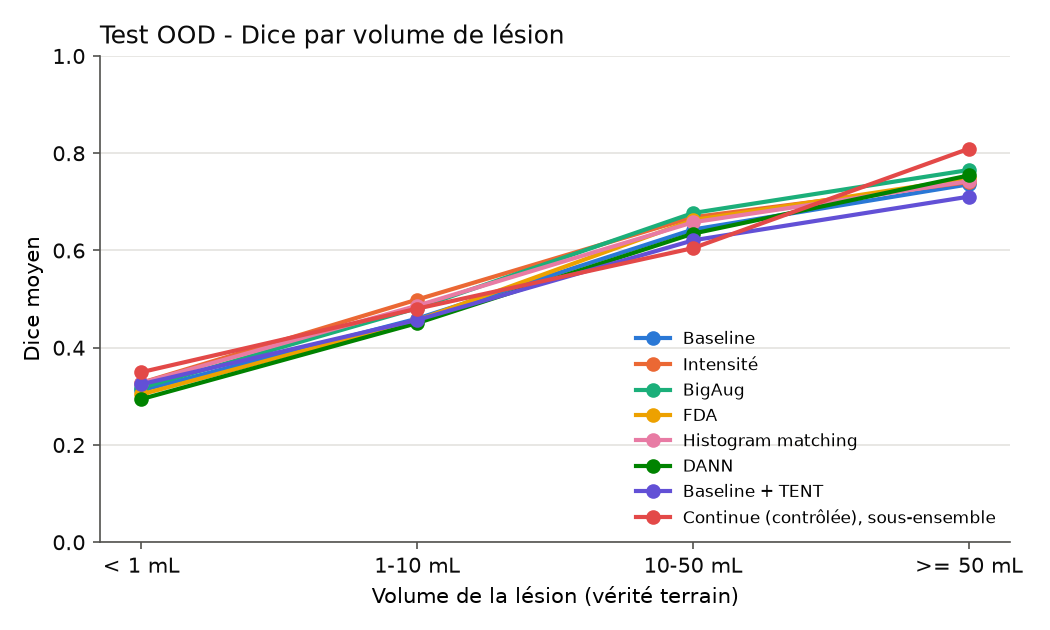
\includegraphics[width=0.8\linewidth]{figures/rq3/rq3_echecs_dice_par_taille.png}
  \caption{Dice moyen par volume de lésion sur le test OOD, avec l'adaptation continue contrôlée (sous-ensemble préquentiel).}
  \label{fig:rq3-echecs-taille}
\end{figure}

\subsection{Centre R008}

Toutes les techniques obtiennent un Dice nul ou presque sur R008. Le Dice moyen de BigAug est de 0,006 sur le centre ; un seul sujet est non nul, à 0,04 (tableau~\ref{tab:rq3-bigaug-intensite} ; moyenne arrondie à 0,01 dans le tableau~\ref{tab:rq3-centres}). Celui d'histogram matching est de 0,019, avec un seul sujet non nul, à 0,13 (tableau~\ref{tab:rq3-hm-intensite}). Le détail par sujet est dans \nolinkurl{zoom_R008_R053.csv}.
\begin{itemize}
  \item Six sujets sur sept sont imagés au premier jour après l'AVC. Leurs lésions font de 0,1 à 4,1~ml.
  \item Les lésions sont peu visibles en T1 : contraste médian de $-0{,}17$, contre $-0{,}50$ à $-0{,}98$ dans les autres centres OOD.
  \item Les intensités sont atypiques : 1,1 à 1,7~\% des voxels du cerveau dépassent $z = 3$, contre 0,003~\% en médiane chez les autres sujets OOD (\nolinkurl{contraste_lesions.csv}).
  \item Le modèle prédit de 0,4 à 33,6~ml répartis en nombreuses composantes, pour une différence du nombre de lésions de 9 à 67.
  \item À l'examen des coupes, vaisseaux, sinus et dure-mère apparaissent hyperintenses.
\end{itemize}
% Les coupes de R008 (figures/rq3/rq3_echecs_coupes_R008.png) ne sont pas incluses :
% ce sont des images ATLAS, non versionnées ; elles se régénèrent avec adaptation/analyse_echecs.py.

\emph{Hypothèse.} La séquence T1 de R008 aurait été acquise après injection de gadolinium, en phase aiguë.
La lésion n'y aurait pas encore le contraste T1 des lésions chroniques, majoritaires à l'entraînement.
Le décalage serait alors à la fois d'acquisition et de stade clinique.
Cette hypothèse reste à vérifier sur le protocole d'acquisition de R008 et sur l'écart entre la date de l'IRM et celle de l'annotation.

\subsection{Centre R053}

Le Dice moyen de R053 est de 0,20 sur quatre sujets ; un cinquième sujet a un masque vide et est exclu du Dice.
Deux lésions minuscules (0,13 et 0,015~ml) ont un Dice de 0. Les deux autres (1,5 et 2,6~ml) obtiennent 0,27 et 0,52.
Les intensités sont dans la norme (99\textsuperscript{e} centile du z-score proche de 1,8) et le contraste vaut $-0{,}50$.
L'échec s'explique par la taille des lésions, pas par un décalage d'intensité. Avec quatre sujets, la moyenne du centre est très instable.

\subsection{Distance de domaine}

La distance de Wasserstein entre histogrammes d'intensité (\nolinkurl{analysis/center_distance.py}, référence = tous les autres centres) ne prédit pas le Dice dans nos runs (\nolinkurl{spearman.csv}).
\begin{itemize}
  \item Sur les six centres OOD, $\rho$ va de $-0{,}43$ à $-0{,}03$ selon la technique ($p$ de 0,40 à 0,96). Avec la MMD, $\rho$ va de $-0{,}37$ à $-0{,}09$.
  \item Sur les 44 centres de test (ID et OOD), $\rho$ va de 0,03 à 0,12 ($p \geq 0{,}44$).
\end{itemize}
La figure~\ref{fig:rq3-distance} en donne deux contre-exemples. R053 est l'un des centres les plus proches (0,020) et l'un des pires. R031 est éloigné (0,164) et parmi les meilleurs.
Six centres offrent une puissance très faible : nous ne concluons pas à l'absence de lien, seulement qu'il n'apparaît pas ici.

\begin{figure}[htbp]
  \centering
  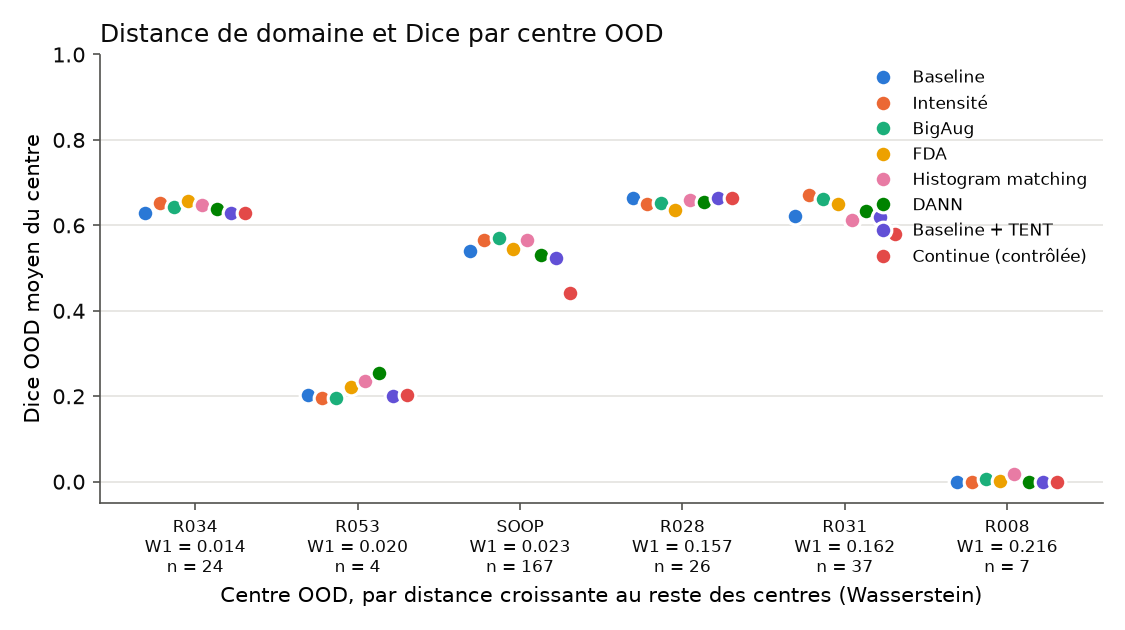
\includegraphics[width=0.8\linewidth]{figures/rq3/rq3_echecs_distance_dice.png}
  \caption{Dice OOD moyen par centre, les centres étant rangés par distance croissante au reste des centres.}
  \label{fig:rq3-distance}
\end{figure}

Au niveau des sujets, le contraste de la lésion n'est que faiblement lié au Dice ($\rho = -0{,}19$, $p = 0{,}001$). La figure~\ref{fig:rq3-contraste} montre ce nuage et place les sujets de R008 et R053.

\begin{figure}[htbp]
  \centering
  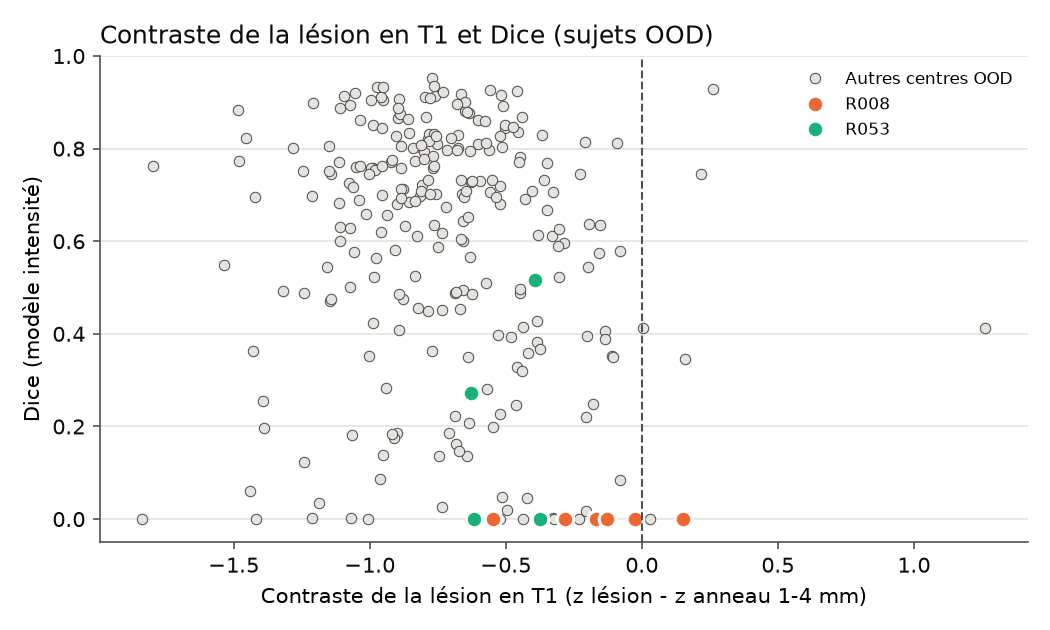
\includegraphics[width=0.8\linewidth]{figures/rq3/rq3_echecs_contraste_dice.png}
  \caption{Contraste T1 de la lésion et Dice (modèle intensité) pour les sujets OOD ; R008 et R053 sont mis en évidence.}
  \label{fig:rq3-contraste}
\end{figure}

\section{Adaptation continue contrôlée}
\label{sec:rq3-continue}

\paragraph{Protocole.}
L'expérience est réalisée par le script \nolinkurl{adaptation/continual.py}.
Ses sorties se trouvent dans le dossier \nolinkurl{adaptation/outputs/rq3/adaptation_continue/}.
Le modèle baseline reçoit les six centres OOD l'un après l'autre, par lots de quatre sujets : 28 lots, 108 sujets, au plus 24 par centre. Il n'est jamais réinitialisé.
L'évaluation est préquentielle : chaque lot est d'abord noté (Dice), puis utilisé pour l'adaptation, sans étiquettes.
Quatre stratégies sont comparées sur les mêmes lots :
\begin{itemize}
  \item \texttt{fige} : le modèle reste inchangé ;
  \item \texttt{auto\_apprentissage} : pseudo-étiquettes, tous les poids sont mis à jour ;
  \item \texttt{tent} : TENT appliqué en continu ;
  \item \texttt{controlee} : TENT dans un modèle candidat, promu seulement si trois conditions sont réunies. (1) La distance du lot dépasse un seuil calibré sur la source (0,077). (2) L'entropie baisse sur des patches neufs. (3) Le Dice sur un jeu de garde étiqueté de la source ne baisse pas de plus de 0,01. Cette stratégie rejoue aussi des exemples des centres déjà vus et des patches de la source.
\end{itemize}
L'oubli est mesuré après chaque centre, par le Dice sur 16 sujets fixes du test ID et sur les premiers sujets des centres OOD déjà vus.

\paragraph{Résultats.}
Le tableau~\ref{tab:rq3-continue} résume les quatre stratégies (\nolinkurl{resume.json}, \nolinkurl{oubli.csv}).

\begin{table}[htbp]
  \centering
  \caption{Adaptation continue sur les six centres OOD : Dice préquentiel et oubli.}
  \label{tab:rq3-continue}
  \small
  \begin{tabular}{lcccc}
    \toprule
    Stratégie & \makecell{Dice\\préquentiel} & \makecell{Dice ID\\(début $\rightarrow$ fin)} & Oubli ID & \makecell{Oubli OOD\\moyen} \\
    \midrule
    Figé & 0,528 & 0,635 $\rightarrow$ 0,635 & 0,000 & 0,000 \\
    Auto-apprentissage & 0,486 & 0,635 $\rightarrow$ 0,583 & 0,052 & 0,033 \\
    TENT continu & 0,526 & 0,635 $\rightarrow$ 0,632 & 0,002 & 0,000 \\
    Contrôlée & 0,527 & 0,635 $\rightarrow$ 0,634 & 0,001 & 0,000 \\
    \bottomrule
  \end{tabular}
\end{table}

Les décisions lot par lot sont dans \nolinkurl{decisions.csv}.
\begin{itemize}
  \item \textbf{Détection.} Un décalage est détecté sur 15 lots sur 28 : tous ceux de R008, R028 et R031, et un lot sur six de SOOP. Il n'est jamais détecté sur R034 ni R053, les centres les plus proches de la source.
  \item \textbf{Promotions.} Douze candidats sont promus : deux pour R008, six pour R028, trois pour R031 et un pour SOOP. Trois candidats de R031 sont refusés parce que leur entropie augmente.
  \item \textbf{Oubli.} La stratégie contrôlée évite l'oubli de l'auto-apprentissage (0,001 contre 0,052 sur le test ID).
  \item \textbf{Gain.} Elle n'améliore pas le Dice par rapport au modèle figé (0,527 contre 0,528).
\end{itemize}

\paragraph{Lecture du résultat.}
L'absence de gain s'explique par la nature des décalages détectés.
R028 et R031 sont déjà bien segmentés par le modèle figé (0,66 et 0,58 en préquentiel).
Sur R008, le problème tient au contraste des lésions (section~\ref{sec:rq3-echecs}), qu'une adaptation des normalisations ne peut pas créer.
Les Dice préquentiels portent sur 108 des 268 sujets OOD ; ils ne se comparent pas directement au tableau~\ref{tab:rq3-resultats}.

\section{Limites}
\label{sec:rq3-limites}

\begin{itemize}
  \item \textbf{Un seul pli et une seule graine.} Les IC traduisent la variabilité des sujets, pas celle de l'entraînement.
  \item \textbf{Reprise de DANN.} La run a été coupée à l'itération 35\,889 et reprise jusqu'à 40\,000. La reprise restaure les poids, l'optimiseur, le taux d'apprentissage, $\lambda$, la position de l'échantillonneur et les états aléatoires des processus de chargement. Le contrôle automatique a validé la première ligne reprise (itération 35\,900, taux $1{,}29 \times 10^{-4}$, $\lambda = 0{,}9771$). Seuls les masques de Dropout du classifieur de centre ne sont pas restaurés. Le meilleur modèle, à l'itération 24\,000, précède de toute façon la coupure.
  \item \textbf{Environnement de DANN.} DANN a été entraînée sur Colab avec torch 2.14.1+cu130 jusqu'à l'itération 35\,889, puis sur Kaggle avec torch 2.11.0+cu130, comme les autres runs. Les deux plateformes utilisent un GPU T4 et CUDA 13.0. Le meilleur modèle (itération 24\,000) vient de la partie Colab. La différence de version de torch peut changer les calculs numériques ; son effet n'a pas été mesuré.
  \item \textbf{Poids de DANN.} Avec un poids de 1, la première run DANN a divergé (perte totale de 10\,508 à l'itération 100 et de 33 millions à l'itération 400). Le poids de 0,1 et la LayerNorm ont été choisis pour la stabilité, sans recherche d'hyperparamètres. Un autre poids pourrait donner un autre résultat.
  \item \textbf{Validation sur des centres non vus.} Ses lésions sont plus petites que celles du test. Elle sert à choisir le checkpoint, mais son Dice (environ 0,43) n'estime pas la performance ID.
  \item \textbf{Diagnostic fp16.} La première baseline, entraînée en fp16, a produit des NaN : des patches entiers donnaient des logits NaN dès l'itération 160 à 180 environ, alors que le fp32 restait stable sur les mêmes lots. Toutes les runs ont été refaites en fp32, environ deux fois plus lentement. La couche qui déborde n'a pas été localisée.
  \item \textbf{Bug de reprise corrigé.} Dans la version du code utilisée pour les runs, la ligne de progression écrasait la file des états aléatoires sauvegardés pour la reprise. Le défaut ne concerne que les reprises, donc uniquement DANN. Il a été corrigé et couvert par un test. Le checkpoint de DANN a été réparé avant la reprise en ne gardant que les quatre derniers états, qui étaient les bons ; les poids n'ont pas changé.
  \item \textbf{Référence de la distance de domaine.} Pour chaque centre, la référence de \nolinkurl{center_distance} regroupe tous les autres centres, OOD compris, et pas seulement les centres d'entraînement du pli~0. La distance mesure donc l'écart au reste du jeu de données, pas exactement l'écart à ce que le modèle a vu.
  \item \textbf{Version du code d'histogram matching.} Cette run a utilisé une version ultérieure du code (\texttt{dbf2f28} au lieu de \texttt{7449c49}), qui ne diffère que par la correction du bug de reprise. Sans DANN ni reprise, les deux versions donnent des poids identiques (vérifié par un court entraînement sur CPU, pour la baseline et l'intensité).
  \item \textbf{Quota GPU.} Avec 30~h par semaine sur Kaggle, aucun autre pli n'a été entraîné, et l'histogram matching a été lancé après les autres techniques.
  \item \textbf{Portée de TENT et de l'adaptation continue.} Les deux ne sont évalués que sur la baseline.
\end{itemize}

\section{Conclusion}
\label{sec:rq3-conclusion}

Sur le pli~0, seule l'augmentation d'intensité améliore le Dice OOD de façon significative après correction : $+0{,}024$ [0,008 ; 0,041], $p$ Holm $= 0{,}0068$ (tableau~\ref{tab:rq3-resultats}).
BigAug atteint le même Dice OOD (0,577), mais son gain n'est pas significatif après correction ($p$ Holm $= 0{,}14$), et la comparaison directe ne sépare pas les deux techniques ($+0{,}001$ [$-0{,}010$ ; 0,012], tableau~\ref{tab:rq3-bigaug-intensite}).
Histogram matching n'est pas significatif non plus ($+0{,}017$, $p$ Holm $= 0{,}49$) ; il reste en dessous de l'intensité en Dice OOD ($-0{,}007$ [$-0{,}023$ ; 0,009]), avec un écart net sur R031 (tableau~\ref{tab:rq3-hm-intensite}).
Aucune technique ne supprime l'écart ID $-$ OOD, qui reste compris entre 0,075 et 0,104.
FDA, DANN et TENT n'améliorent pas le test OOD ; TENT le dégrade légèrement.
L'adaptation continue contrôlée évite l'oubli sans améliorer le Dice (tableau~\ref{tab:rq3-continue}).
L'analyse des échecs montre que les cas les plus difficiles tiennent aux lésions elles-mêmes, petites ou peu contrastées en T1, plutôt qu'à la distance d'intensité entre centres.
Le livrable C8 (\nolinkurl{adaptation/inference.py}) segmente un T1 et renvoie le masque et le volume de la lésion.
Le modèle retenu pour la démonstration est celui de l'intensité.
À Dice égal avec BigAug, ce choix repose d'abord sur son gain significatif après correction, ensuite sur un entraînement plus court (5,0~h contre 8,1~h).
Son F1 des lésions est supérieur à celui de BigAug (0,450 contre 0,420) mais inférieur à celui de la baseline (0,477) : ce n'est qu'un argument relatif face à BigAug.
Histogram matching a le plus faible écart absolu de volume (9,1~ml contre 10,0~ml pour l'intensité) et un F1 des lésions supérieur à celui de la baseline (0,486 contre 0,477).
Il n'a pas été retenu, car son gain en Dice n'est pas significatif et il exigerait d'harmoniser aussi chaque volume à l'inférence, avec l'histogramme de référence de R059.
Ces constats orientent la suite vers la prédiction des cas à risque, en particulier les lésions de moins de 1~ml et les AVC en phase aiguë.
.
% Paquets attendus dans le préambule : babel (french), graphicx, booktabs, makecell, hyperref, float.
% Réglages à mettre dans le préambule du rapport final :
%   \addto\captionsfrench{\def\tablename{Tableau}}   % « Tableau » au lieu de « Table »
%   \hypersetup{hidelinks}                             % liens sans cadre rouge
% Les chemins des figures sont relatifs à la racine du dépôt.
% Citations : docs/rapport/references_rq3.bib, à ajouter à la commande \bibliography du rapport.

\chapter{Généralisation inter-centres (RQ3) et adaptation continue contrôlée}
\label{chap:rq3}

\section{Introduction}
\label{sec:rq3-introduction}

Ce chapitre étudie la robustesse d'un modèle de segmentation des lésions d'AVC face à des centres d'acquisition jamais vus.
La question de recherche RQ3 est la suivante : « Quelles techniques de data augmentation et/ou d'adaptation de domaine réduisent le plus efficacement l'écart de performance entre centres ? »
Nous mesurons cet écart entre des centres vus à l'entraînement (ID) et des centres non vus (OOD).
Nous décrivons d'abord le protocole et les techniques évaluées, puis les résultats et l'analyse des échecs.
Nous présentons ensuite une adaptation continue contrôlée, avant de discuter les limites de l'étude.

\section{Protocole expérimental}
\label{sec:rq3-protocole}

\paragraph{Données.}
Nous utilisons les images T1 d'ATLAS v2.0~\cite{liew2022atlas}, déjà débarrassées du crâne, après le prétraitement S4 de l'équipe : orientation RAS, rééchantillonnage à 1~mm, recadrage sur le cerveau et z-score dans le cerveau (\nolinkurl{preprocessing/week4.py}).
Le découpage est fixé dans \nolinkurl{splits.json}. Le centre R032 est exclu.

\paragraph{Découpage par centre.}
Six centres sont réservés au test OOD : R008, R028, R031, R034, R053 et SOOP.
Ils ont été choisis sur la taille des centres et la distance entre histogrammes d'intensité, sans consulter le Dice (champ \texttt{selection} de \nolinkurl{splits.json}).
Les autres centres sont répartis en cinq plis. Seul le pli~0 a été entraîné. Le tableau~\ref{tab:rq3-donnees} donne les effectifs.

\begin{table}[htbp]
  \centering
  \caption{Effectifs du pli~0.}
  \label{tab:rq3-donnees}
  \begin{tabular}{lrl}
    \toprule
    Ensemble & Sujets & Centres \\
    \midrule
    Entraînement & 733 & 39 \\
    Validation & 183 & 9 centres absents de l'entraînement \\
    Test ID & 185 & centres d'entraînement, sujets non vus \\
    Test OOD & 268 (265 à lésion non vide) & 6 \\
    \bottomrule
  \end{tabular}
\end{table}

Le découpage de \nolinkurl{splits.json} compte 184 sujets de validation.
L'un d'eux, le sujet r065s019 du centre R065, n'a pas de volume prétraité.
Le prétraitement S4 l'a rejeté, car une partie de sa lésion sort du recadrage calculé sur l'image.
Le chargeur l'écarte, et la validation porte donc sur 183 sujets, comme l'indiquent les journaux d'entraînement.
Un de ces 183 sujets a un masque vide : le Dice de validation est calculé sur 182 sujets.

\paragraph{Modèle et entraînement.}
Le réseau est un U-Net~3D de MONAI~\cite{cardoso2022monai} : canaux de 32 à 320, quatre sous-échantillonnages et deux unités résiduelles par niveau.
La normalisation d'instance est affine, ce qu'exige TENT.
L'entraînement utilise des patches de $96^3$ voxels, par lots de quatre patches (deux volumes $\times$ deux patches), dont la moitié est centrée sur la lésion.
Un miroir gauche-droite aléatoire est appliqué à toutes les runs.
La perte combine Dice et entropie croisée.
L'optimiseur AdamW part d'un taux d'apprentissage de $10^{-3}$, avec une décroissance polynomiale (puissance 0,9) et une décroissance des poids de $10^{-5}$.
La norme des gradients est écrêtée à 12.
Toutes les techniques reçoivent le même budget : 40\,000 itérations, graine 2026, calcul en fp32 sur un GPU T4.
Les runs ont été exécutées sur Kaggle (torch 2.11.0+cu130), sauf DANN.
DANN a été entraînée sur Google Colab (GPU T4, torch 2.14.1+cu130) jusqu'à l'itération 35\,889, puis reprise sur Kaggle jusqu'à 40\,000 (section~\ref{sec:rq3-limites}).

\paragraph{Sélection du modèle.}
Le modèle est validé toutes les 2\,000 itérations sur les 183 sujets de validation, en volume entier, par fenêtre glissante de $96^3$ (recouvrement 0,25).
Le checkpoint retenu est celui du meilleur Dice de validation. Il est évalué une seule fois sur les tests ID et OOD.

\paragraph{Métriques.}
Nous rapportons le Dice, la distance de Hausdorff à 95~\% (HD95), l'écart absolu de volume, le F1 des lésions et la différence du nombre de lésions.
Ces métriques sont communes à l'équipe (\nolinkurl{baselines/common.py}).
Le Dice n'est calculé que sur les sujets dont la lésion n'est pas vide.

\paragraph{Tests statistiques.}
Les moyennes sont données avec un intervalle de confiance (IC) à 95~\% par bootstrap percentile (10\,000 tirages).
Pour l'écart ID $-$ OOD, les deux groupes sont rééchantillonnés indépendamment.
Chaque technique est comparée à la baseline par un test des rangs signés de Wilcoxon~\cite{wilcoxon1945}, apparié sur les mêmes sujets.
Une correction de Holm~\cite{holm1979} est appliquée sur l'ensemble des techniques comparées.
La correction porte sur six comparaisons : intensité, BigAug, FDA, histogram matching, DANN et TENT.
BigAug et histogram matching sont aussi comparés directement à l'intensité (différence appariée, IC bootstrap, Wilcoxon), hors correction de Holm : ce sont des comparaisons secondaires avec la technique de référence.

\section{Techniques évaluées}
\label{sec:rq3-techniques}

Toutes les techniques partagent le réseau, les plis, les graines et le budget d'itérations. Seule l'étape propre à chaque technique change (\nolinkurl{adaptation/train.py}, \nolinkurl{generalization/configs/}).

\begin{itemize}
  \item \textbf{Augmentation d'intensité.} Gamma ($p = 0{,}3$) et contraste ($p = 0{,}3$), calibrés sur les seuls sujets d'entraînement ; bruit ($p = 0{,}2$), flou ($p = 0{,}2$), champ de biais ($p = 0{,}3$) et basse résolution ($p = 0{,}25$, jusqu'à 3~mm sur un axe).
  \item \textbf{BigAug}~\cite{zhang2020bigaug}. Flou, netteté, bruit, luminosité, gamma (plage calibrée) et transformation affine (échelle de 0,8 à 1,2, rotation de 20\textdegree), chacun avec $p = 0{,}5$. La déformation élastique est désactivée. Les plages sont adoucies par rapport à l'article pour préserver les petites lésions.
  \item \textbf{FDA} (Fourier Domain Adaptation)~\cite{yang2020fda}. L'amplitude basse fréquence est échangée avec celle d'une image d'un centre d'entraînement de référence (R059 pour le pli~0), avec $\beta$ entre 0,015 et 0,03 et $p = 0{,}5$.
  \item \textbf{DANN} (Domain-Adversarial Neural Network)~\cite{ganin2016dann}. Un classifieur des 39 centres d'entraînement est branché sur la sortie du goulot du réseau : moyenne spatiale, LayerNorm sans paramètres, puis perceptron de 64 unités. Une couche d'inversion du gradient le relie à l'encodeur. Le coefficient $\lambda$ est nul pendant les 2\,000 premières itérations, puis suit la montée proposée par Ganin et al.\ ($\gamma = 5$). La perte du centre a un poids de 0,1.
  \item \textbf{TENT}~\cite{wang2021tent}. Adaptation au test, sans étiquettes, du modèle baseline. Seuls les paramètres affines des normalisations sont modifiés, en minimisant l'entropie des prédictions, centre par centre (Adam, taux de $10^{-4}$, quatre patches par sujet).
  \item \textbf{Histogram matching.} L'histogramme d'intensité du cerveau de chaque volume est ramené vers un histogramme de référence, moyenné sur 20 sujets d'un centre d'entraînement (R059 pour le pli~0). La transformation est déterministe ($p = 1$) et s'applique aussi à la validation et au test. Faute de quota GPU, cette run a été lancée après les autres, avec une version ultérieure du code (section~\ref{sec:rq3-limites}).
\end{itemize}
Fan-Net~\cite{yu2023fannet} n'a pas été implémenté ; FDA en reprend le principe (échange d'amplitude de Fourier) sous une forme plus simple.

\section{Résultats RQ3}
\label{sec:rq3-resultats}

Le tableau~\ref{tab:rq3-resultats} résume les résultats sur 185 sujets ID et 265 sujets OOD (\nolinkurl{adaptation/outputs/rq3/tableau_rq3.md}).

\begin{table}[htbp]
  \centering
  \caption{Dice moyen par technique (pli~0), avec l'IC à 95~\% sous chaque valeur. $\Delta$ OOD : différence appariée à la baseline sur le test OOD ; $p$ : test de Wilcoxon, puis $p$ corrigé par Holm.}
  \label{tab:rq3-resultats}
  \small
  \setlength{\tabcolsep}{4pt}
  \begin{tabular}{lccccc}
    \toprule
    Technique & Dice ID & Dice OOD & \makecell{Écart\\ID $-$ OOD} & $\Delta$ OOD & $p$ OOD \\
    \midrule
    Baseline & \makecell{0,646\\{\footnotesize [0,611 ; 0,680]}} & \makecell{0,553\\{\footnotesize [0,517 ; 0,589]}} & \makecell{0,093\\{\footnotesize [0,044 ; 0,142]}} & -- & -- \\[2pt]
    Intensité & \makecell{0,656\\{\footnotesize [0,621 ; 0,690]}} & \makecell{0,577\\{\footnotesize [0,543 ; 0,611]}} & \makecell{0,080\\{\footnotesize [0,031 ; 0,126]}} & \makecell{+0,024\\{\footnotesize [0,008 ; 0,041]}} & \makecell{0,0014\\{\footnotesize (Holm 0,0068)}} \\[2pt]
    BigAug & \makecell{0,653\\{\footnotesize [0,619 ; 0,686]}} & \makecell{0,577\\{\footnotesize [0,543 ; 0,611]}} & \makecell{0,075\\{\footnotesize [0,028 ; 0,122]}} & \makecell{+0,025\\{\footnotesize [0,010 ; 0,040]}} & \makecell{0,035\\{\footnotesize (Holm 0,14)}} \\[2pt]
    FDA & \makecell{0,660\\{\footnotesize [0,626 ; 0,693]}} & \makecell{0,559\\{\footnotesize [0,524 ; 0,593]}} & \makecell{0,101\\{\footnotesize [0,053 ; 0,148]}} & \makecell{+0,006\\{\footnotesize [$-$0,007 ; 0,020]}} & \makecell{0,32\\{\footnotesize (Holm 0,49)}} \\[2pt]
    \makecell[l]{Histogram\\matching} & \makecell{0,646\\{\footnotesize [0,611 ; 0,681]}} & \makecell{0,570\\{\footnotesize [0,536 ; 0,604]}} & \makecell{0,077\\{\footnotesize [0,027 ; 0,125]}} & \makecell{+0,017\\{\footnotesize [0,001 ; 0,034]}} & \makecell{0,24\\{\footnotesize (Holm 0,49)}} \\[2pt]
    DANN & \makecell{0,650\\{\footnotesize [0,616 ; 0,684]}} & \makecell{0,549\\{\footnotesize [0,513 ; 0,584]}} & \makecell{0,102\\{\footnotesize [0,053 ; 0,150]}} & \makecell{$-$0,004\\{\footnotesize [$-$0,018 ; 0,009]}} & \makecell{0,13\\{\footnotesize (Holm 0,39)}} \\[2pt]
    \makecell[l]{Baseline\\+ TENT} & \makecell{0,645\\{\footnotesize [0,610 ; 0,679]}} & \makecell{0,542\\{\footnotesize [0,506 ; 0,578]}} & \makecell{0,104\\{\footnotesize [0,054 ; 0,153]}} & \makecell{$-$0,011\\{\footnotesize [$-$0,016 ; $-$0,006]}} & \makecell{$< 10^{-4}$\\{\footnotesize (Holm $< 10^{-4}$)}} \\[2pt]
    \bottomrule
  \end{tabular}
\end{table}

La figure~\ref{fig:rq3-dice-id-ood} montre les Dice ID et OOD de chaque technique avec leurs IC.
L'écart entre ID et OOD demeure pour toutes les techniques : il va de 0,075 à 0,104, et aucun IC ne contient 0.

\begin{figure}[htbp]
  \centering
  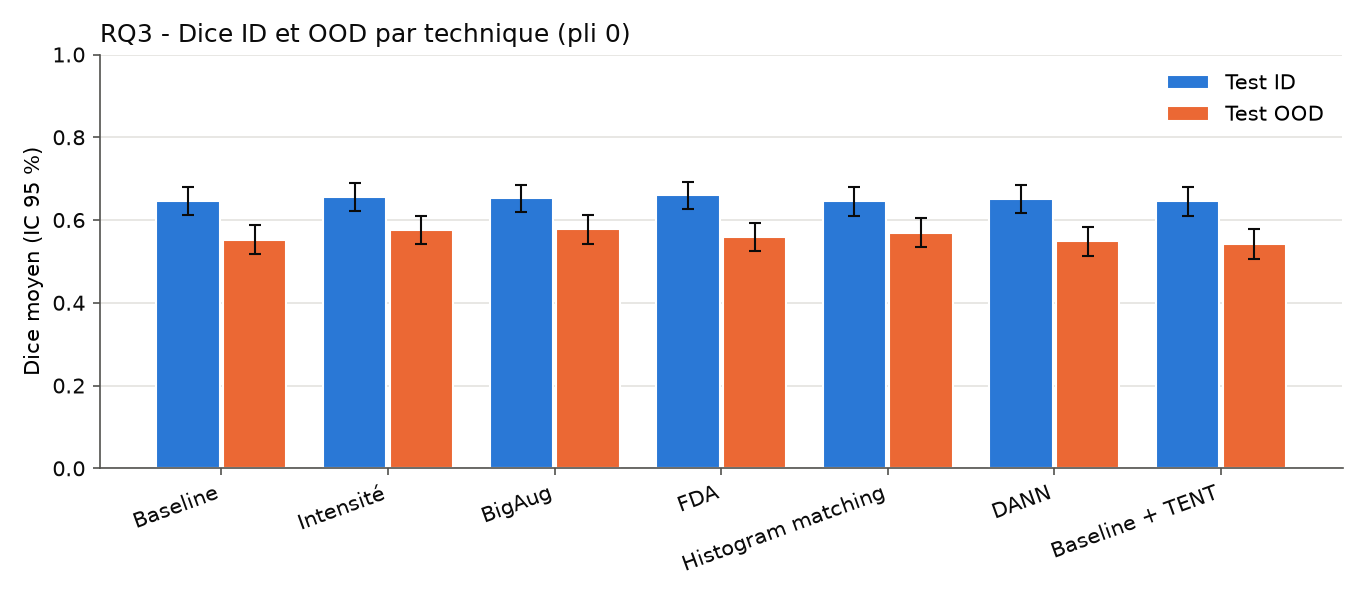
\includegraphics[width=0.8\linewidth]{figures/rq3/rq3_dice_id_ood.png}
  \caption{Dice moyen sur les tests ID et OOD par technique, avec IC à 95~\% (pli~0).}
  \label{fig:rq3-dice-id-ood}
\end{figure}

La figure~\ref{fig:rq3-delta-ood} montre la distribution des différences appariées à la baseline sur le test OOD.
\begin{itemize}
  \item L'augmentation d'intensité est la seule technique qui améliore le Dice OOD de façon significative après correction : $+0{,}024$ [0,008 ; 0,041], $p = 0{,}0014$, $p$ Holm $= 0{,}0068$. Le gain est réparti : 155 sujets sur 252 différences non nulles sont en sa faveur, pour une médiane de $+0{,}006$.
  \item BigAug obtient le même gain moyen ($+0{,}025$ [0,010 ; 0,040]), mais son Wilcoxon ($p = 0{,}035$) n'est plus significatif après correction ($p$ Holm $= 0{,}14$). La différence médiane avec la baseline est quasi nulle ($+0{,}001$ ; 135 sujets en sa faveur sur 250 différences non nulles), et la moyenne est tirée par quelques grands écarts, jusqu'à $+0{,}67$. C'est ce qui explique que le Wilcoxon, fondé sur les rangs, ne passe pas la correction de Holm. Son écart ID $-$ OOD est le plus faible (0,075), mais son IC chevauche celui de la baseline.
  \item FDA a le meilleur Dice ID (0,660), mais son gain sur la baseline n'est significatif après correction ni en ID (Wilcoxon $p = 0{,}012$, $p$ Holm $= 0{,}061$ ; $\Delta$ ID $= +0{,}014$ [$-$0,001 ; 0,029]), ni en OOD ($p = 0{,}32$).
  Avant correction, le Wilcoxon en ID est significatif alors que l'IC bootstrap de $\Delta$ ID contient 0, car les deux ne testent pas la même chose.
  Le Wilcoxon porte sur les rangs des différences appariées : 109 sujets sur 179 différences non nulles sont en faveur de FDA, pour une médiane de $+0{,}005$.
  L'IC porte sur la moyenne, que quelques grandes différences dans les deux sens (jusqu'à $-0{,}32$) rendent plus variable.
  \item Histogram matching améliore le Dice OOD en moyenne ($+0{,}017$ [0,001 ; 0,034]), mais pas de façon significative ($p = 0{,}24$, $p$ Holm $= 0{,}49$). L'IC bootstrap de $\Delta$ OOD exclut tout juste 0 alors que le Wilcoxon n'est pas significatif, pour la même raison que FDA en ID : l'IC porte sur la moyenne, tirée par quelques grands écarts (jusqu'à $+0{,}84$), et le Wilcoxon sur les rangs, avec une médiane nulle (125 sujets en sa faveur, 125 en sa défaveur). Son écart ID $-$ OOD (0,077) est proche de celui de BigAug.
  \item DANN ne se distingue de la baseline ni en ID ($p = 0{,}45$) ni en OOD ($p = 0{,}13$).
  \item TENT abaisse le Dice OOD de 0,011 [0,006 ; 0,016]. L'effet est petit mais systématique ($p < 10^{-4}$). En ID, la baisse est de 0,0007 [0,0002 ; 0,0012] ($p = 1{,}7 \times 10^{-4}$, $p$ Holm $= 1{,}0 \times 10^{-3}$).
\end{itemize}

\begin{figure}[htbp]
  \centering
  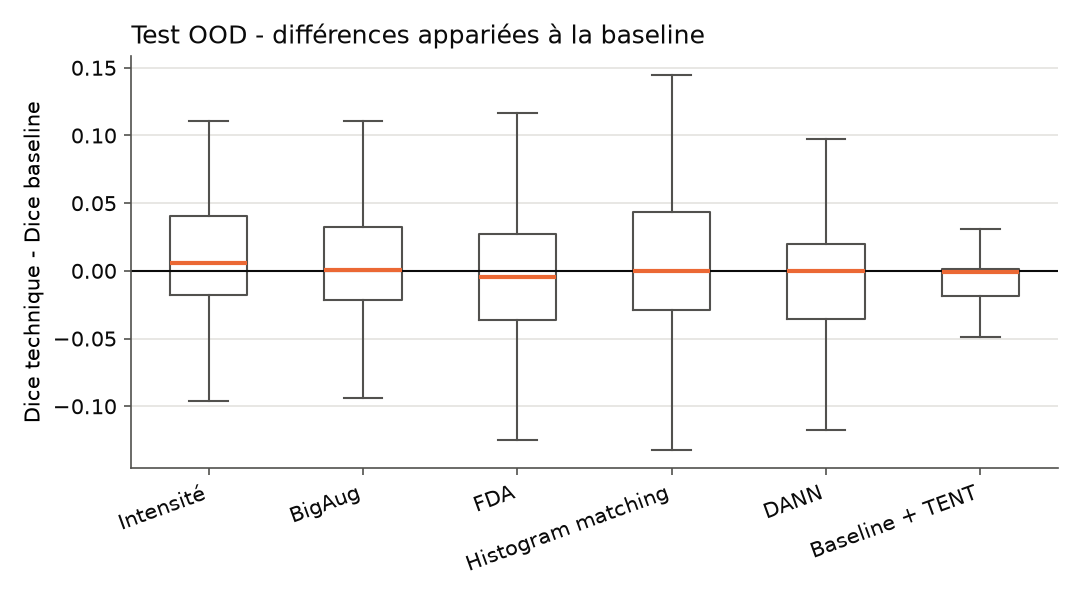
\includegraphics[width=0.8\linewidth]{figures/rq3/rq3_delta_ood.png}
  \caption{Différences appariées de Dice avec la baseline, par sujet, sur le test OOD.}
  \label{fig:rq3-delta-ood}
\end{figure}

\paragraph{BigAug et intensité.}
Le tableau~\ref{tab:rq3-bigaug-intensite} compare directement les deux techniques sur les mêmes sujets (\nolinkurl{adaptation/outputs/rq3/comparaisons.csv}).
Sur le test OOD, la différence moyenne BigAug $-$ intensité vaut $+0{,}001$ [$-0{,}010$ ; 0,012] ($p = 0{,}53$ ; 123 sujets en faveur de BigAug, 128 en faveur de l'intensité).
Sur le test ID, elle vaut $-0{,}003$ [$-0{,}017$ ; 0,011] ($p = 0{,}35$).
Aucun centre OOD ne les sépare : les différences vont de $-0{,}011$ (R034) à $+0{,}006$ (R008), toutes avec $p \geq 0{,}32$.
Les deux techniques sont donc équivalentes en Dice à la précision de cette étude.
Elles diffèrent sur deux points secondaires.
L'entraînement de BigAug dure 8,1~h contre 5,0~h pour l'intensité (\nolinkurl{adaptation/outputs/rq3/entrainement.csv}).
Le F1 des lésions OOD est plus élevé avec l'intensité qu'avec BigAug (0,450 contre 0,420), mais les deux restent sous la baseline (0,477, tableau~\ref{tab:rq3-secondaires}) : ce n'est qu'un avantage relatif face à BigAug.

\begin{table}[htbp]
  \centering
  \caption{Comparaison directe BigAug $-$ intensité par centre OOD (sujets appariés). Source : \texttt{comparaisons\_par\_centre.csv}.}
  \label{tab:rq3-bigaug-intensite}
  \small
  \setlength{\tabcolsep}{4pt}
  \begin{tabular}{lcccccc}
    \toprule
    Centre & n & Dice BigAug & Dice intensité & $\Delta$ moyen & \makecell{Sujets\\BigAug > / < intensité} & $p$ Wilcoxon \\
    \midrule
    R008 & 7 & 0,006 & 0,000 & +0,006 & 1 / 0 & 1 \\
    R028 & 26 & 0,652 & 0,649 & +0,003 & 16 / 10 & 0,50 \\
    R031 & 37 & 0,663 & 0,672 & $-$0,009 & 15 / 22 & 0,32 \\
    R034 & 24 & 0,642 & 0,653 & $-$0,011 & 11 / 12 & 0,76 \\
    R053 & 4 & 0,195 & 0,197 & $-$0,002 & 1 / 1 & 1 \\
    SOOP & 167 & 0,571 & 0,567 & +0,004 & 79 / 83 & 0,60 \\
    \midrule
    Total OOD & 265 & 0,577 & 0,577 & +0,001 & 123 / 128 & 0,53 \\
    \bottomrule
  \end{tabular}
\end{table}

\paragraph{Histogram matching et intensité.}
Le tableau~\ref{tab:rq3-hm-intensite} compare de la même façon histogram matching et intensité.
Sur le test OOD, la différence moyenne histogram matching $-$ intensité vaut $-0{,}007$ [$-0{,}023$ ; 0,009] ($p = 0{,}062$ ; 110 sujets en faveur d'histogram matching, 142 en faveur de l'intensité).
Sur le test ID, elle vaut $-0{,}010$ [$-0{,}025$ ; 0,005] ($p = 0{,}35$).
Le seul écart net par centre concerne R031 : $-0{,}059$ ($p = 0{,}0018$ ; 10 sujets contre 27), qui reste sous 0,05 après une correction de Bonferroni sur les six centres.
Histogram matching a en revanche un F1 des lésions OOD supérieur à celui de la baseline (0,486 contre 0,477) et le plus faible écart absolu de volume de toutes les techniques (9,1~ml, tableau~\ref{tab:rq3-secondaires}).

\begin{table}[htbp]
  \centering
  \caption{Comparaison directe histogram matching $-$ intensité par centre OOD (sujets appariés). HM : histogram matching. Source : \texttt{comparaisons\_par\_centre.csv}.}
  \label{tab:rq3-hm-intensite}
  \small
  \setlength{\tabcolsep}{4pt}
  \begin{tabular}{lcccccc}
    \toprule
    Centre & n & Dice HM & Dice intensité & $\Delta$ moyen & \makecell{Sujets\\HM > / < intensité} & $p$ Wilcoxon \\
    \midrule
    R008 & 7 & 0,019 & 0,000 & +0,019 & 1 / 0 & 1 \\
    R028 & 26 & 0,659 & 0,649 & +0,010 & 16 / 9 & 0,23 \\
    R031 & 37 & 0,614 & 0,672 & $-$0,059 & 10 / 27 & 0,0018 \\
    R034 & 24 & 0,648 & 0,653 & $-$0,005 & 14 / 9 & 0,41 \\
    R053 & 4 & 0,237 & 0,197 & +0,040 & 1 / 1 & 1 \\
    SOOP & 167 & 0,566 & 0,567 & 0,000 & 68 / 96 & 0,11 \\
    \midrule
    Total OOD & 265 & 0,570 & 0,577 & $-$0,007 & 110 / 142 & 0,062 \\
    \bottomrule
  \end{tabular}
\end{table}

\paragraph{Lecture des résultats négatifs.}
Les résultats de DANN et de TENT ne sont pas des défaillances techniques. La run DANN est allée à son terme, avec un contrôle de reprise validé (section~\ref{sec:rq3-limites}). TENT a été appliqué au modèle baseline sur les mêmes sujets. Les deux sont évalués comme les autres techniques.
Pour DANN, l'alignement des caractéristiques entre 39 centres n'apporte rien de mesurable.
Une explication compatible avec nos données est que les échecs OOD dépendent surtout de la taille et du contraste des lésions (section~\ref{sec:rq3-echecs}), deux facteurs que l'alignement des centres ne traite pas.
Pour TENT, la minimisation de l'entropie rend les prédictions plus tranchées sans étiquettes. La baisse touche surtout les lésions de plus de 50~ml (0,71 contre 0,74, tableau~\ref{tab:rq3-taille}).

\paragraph{Métriques secondaires.}
Elles ne suivent pas toujours le Dice (tableau~\ref{tab:rq3-secondaires}).
Le F1 des lésions OOD baisse avec l'intensité (0,450 contre 0,477), BigAug (0,420), FDA et DANN (0,366 et 0,367) ; il augmente avec histogram matching (0,486) et TENT (0,495).
L'écart absolu de volume baisse surtout avec histogram matching (9,1~ml contre 11,1~ml), puis avec l'intensité (10,0~ml) et BigAug (10,9~ml).

\begin{table}[htbp]
  \centering
  \caption{Métriques secondaires moyennes sur le test OOD (\texttt{tableau\_rq3.csv}).}
  \label{tab:rq3-secondaires}
  \begin{tabular}{lccc}
    \toprule
    Technique & F1 des lésions & HD95 (mm) & Écart absolu de volume (ml) \\
    \midrule
    Baseline & 0,477 & 24,9 & 11,1 \\
    Intensité & 0,450 & 25,5 & 10,0 \\
    BigAug & 0,420 & 25,4 & 10,9 \\
    FDA & 0,366 & 26,1 & 13,3 \\
    Histogram matching & 0,486 & 24,9 & 9,1 \\
    DANN & 0,367 & 27,2 & 12,1 \\
    Baseline + TENT & 0,495 & 25,9 & 12,1 \\
    \bottomrule
  \end{tabular}
\end{table}

\paragraph{Validation et test.}
Les meilleurs Dice de validation vont de 0,427 à 0,443 (\nolinkurl{adaptation/outputs/rq3/entrainement.csv}). La validation ne départage donc pas les techniques.
Le Dice de validation (environ 0,43) est plus bas que celui du test ID (0,646) pour deux raisons.
La validation porte sur neuf centres non vus.
Ses lésions sont aussi plus petites : médiane de 1,26~ml et 43~\% sous 1~ml, contre 7,56~ml et 18~\% au test ID (volumes \texttt{lesion\_ml} des fichiers \texttt{qc.json}).

\section{Analyse des échecs}
\label{sec:rq3-echecs}

Les tableaux détaillés de cette section sont produits par le script \nolinkurl{adaptation/analyse_echecs.py}.
Ils se trouvent dans le dossier \nolinkurl{adaptation/outputs/rq3/echecs/}.

\subsection{Dice par centre OOD}

Le tableau~\ref{tab:rq3-centres} et la figure~\ref{fig:rq3-dice-centre} donnent le Dice moyen par centre.
Le contraste T1 est la différence entre le z-score moyen de la lésion et celui d'un anneau de 1 à 4~mm autour d'elle. Une lésion chronique est hypo-intense, et son contraste est négatif.

\begin{table}[htbp]
  \centering
  \caption{Centres OOD, rangés par distance décroissante au reste des centres. Vol. : volume médian des lésions ; J : jours après l'AVC (médiane) ; W1 : distance de Wasserstein ; Base. : baseline ; Int. : intensité ; HM : histogram matching ; TENT : baseline + TENT. Source : \texttt{par\_centre\_ood.csv}.}
  \label{tab:rq3-centres}
  \small
  \setlength{\tabcolsep}{3pt}
  \begin{tabular}{lcccccccccccc}
    \toprule
    & & & & & & \multicolumn{7}{c}{Dice moyen} \\
    \cmidrule(lr){7-13}
    Centre & \makecell{Sujets\\(lésion)} & \makecell{Vol.\\(ml)} & J & W1 & Contraste & Base. & Int. & BigAug & FDA & HM & DANN & TENT \\
    \midrule
    R008 & 7 (7) & 0,95 & 1 & 0,216 & $-$0,17 & 0,00 & 0,00 & 0,01 & 0,00 & 0,02 & 0,00 & 0,00 \\
    R031 & 37 (37) & 6,74 & 138 & 0,164 & $-$0,98 & 0,62 & 0,67 & 0,66 & 0,65 & 0,61 & 0,63 & 0,62 \\
    R028 & 26 (26) & 4,94 & 576 & 0,157 & $-$0,82 & 0,66 & 0,65 & 0,65 & 0,64 & 0,66 & 0,65 & 0,66 \\
    SOOP & 169 (167) & 22,75 & -- & 0,023 & $-$0,69 & 0,54 & 0,57 & 0,57 & 0,54 & 0,57 & 0,53 & 0,52 \\
    R053 & 5 (4) & 0,81 & 25 & 0,020 & $-$0,50 & 0,20 & 0,20 & 0,20 & 0,22 & 0,24 & 0,25 & 0,20 \\
    R034 & 24 (24) & 2,38 & 1\,506 & 0,014 & $-$0,64 & 0,63 & 0,65 & 0,64 & 0,66 & 0,65 & 0,64 & 0,63 \\
    \bottomrule
  \end{tabular}
\end{table}

\begin{figure}[htbp]
  \centering
  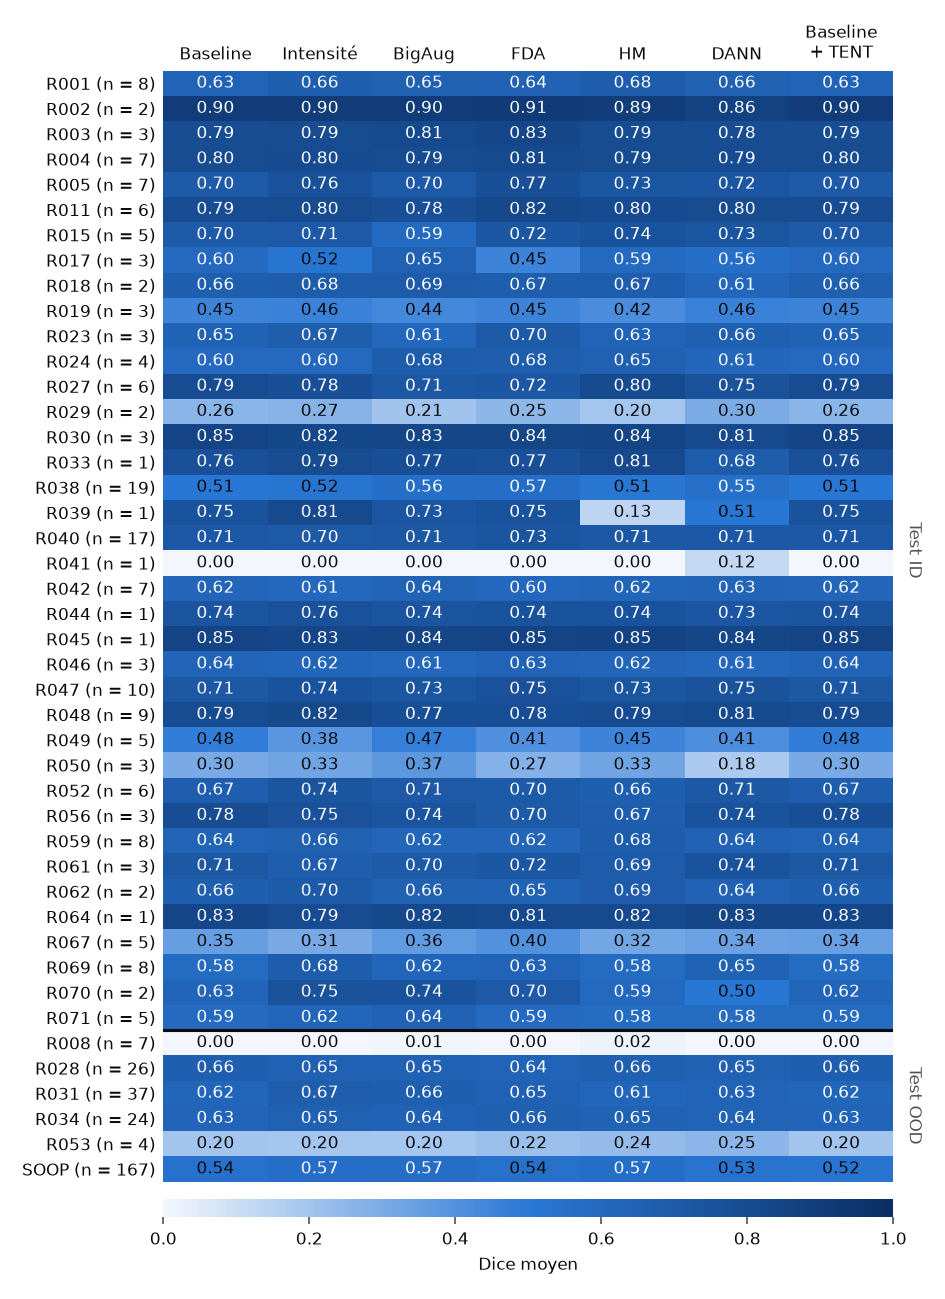
\includegraphics[width=\linewidth]{figures/rq3/rq3_dice_par_centre.png}
  \caption{Dice moyen par centre de test (ID et OOD) et par technique. HM : histogram matching.}
  \label{fig:rq3-dice-centre}
\end{figure}

\subsection{Taille des lésions}

La taille est le facteur le plus net.
Sur les 265 sujets OOD, la corrélation de Spearman entre le volume de la lésion et le Dice (modèle intensité) vaut $\rho = 0{,}53$ ($p < 10^{-4}$).
Le tableau~\ref{tab:rq3-taille} et la figure~\ref{fig:rq3-dice-taille} montrent que toutes les techniques suivent le même profil.
L'intensité gagne surtout entre 1 et 50~ml (0,50 et 0,67 contre 0,46 et 0,64 pour la baseline). BigAug gagne surtout au-dessus de 10~ml (0,68 et 0,77 contre 0,64 et 0,74).

\begin{table}[htbp]
  \centering
  \caption{Dice moyen par volume de lésion sur le test OOD (Dice ID entre parenthèses). L'adaptation continue porte sur un sous-ensemble des sujets.}
  \label{tab:rq3-taille}
  \small
  \begin{tabular}{lcccc}
    \toprule
    Technique & $< 1$~ml & 1--10~ml & 10--50~ml & $\geq 50$~ml \\
    \midrule
    Sujets OOD (ID) & 41 (34) & 86 (65) & 80 (48) & 58 (38) \\
    \midrule
    Baseline & 0,31 (0,48) & 0,46 (0,58) & 0,64 (0,71) & 0,74 (0,83) \\
    Intensité & 0,33 (0,46) & 0,50 (0,59) & 0,67 (0,74) & 0,74 (0,83) \\
    BigAug & 0,32 (0,43) & 0,48 (0,59) & 0,68 (0,75) & 0,77 (0,83) \\
    FDA & 0,30 (0,44) & 0,46 (0,61) & 0,66 (0,74) & 0,75 (0,84) \\
    Histogram matching & 0,33 (0,49) & 0,49 (0,58) & 0,66 (0,71) & 0,74 (0,83) \\
    DANN & 0,29 (0,46) & 0,45 (0,58) & 0,63 (0,73) & 0,75 (0,83) \\
    Baseline + TENT & 0,32 (0,48) & 0,46 (0,58) & 0,62 (0,71) & 0,71 (0,82) \\
    Continue (contrôlée) & 0,35 & 0,48 & 0,60 & 0,81 \\
    \bottomrule
  \end{tabular}
\end{table}

\begin{figure}[htbp]
  \centering
  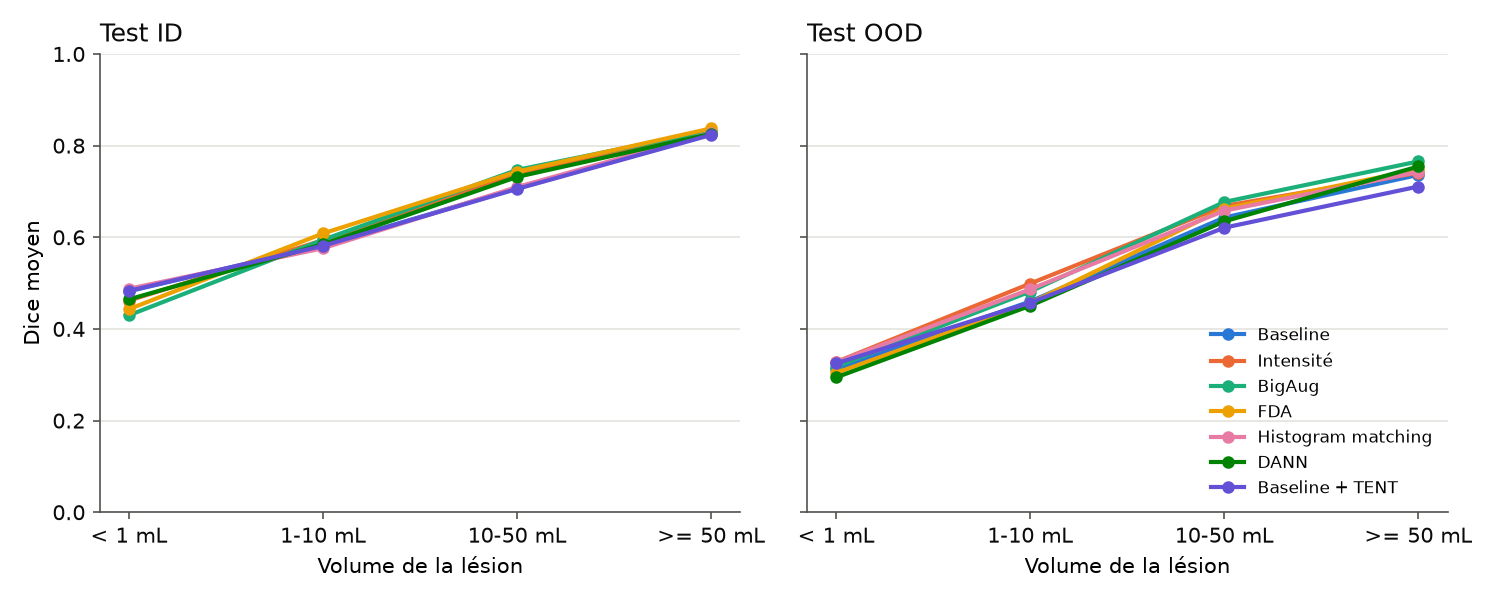
\includegraphics[width=\linewidth]{figures/rq3/rq3_dice_par_taille.png}
  \caption{Dice moyen par classe de volume de lésion, sur les tests ID (à gauche) et OOD (à droite).}
  \label{fig:rq3-dice-taille}
\end{figure}

La figure~\ref{fig:rq3-echecs-taille} reprend le test OOD en y ajoutant l'adaptation continue contrôlée.

\begin{figure}[htbp]
  \centering
  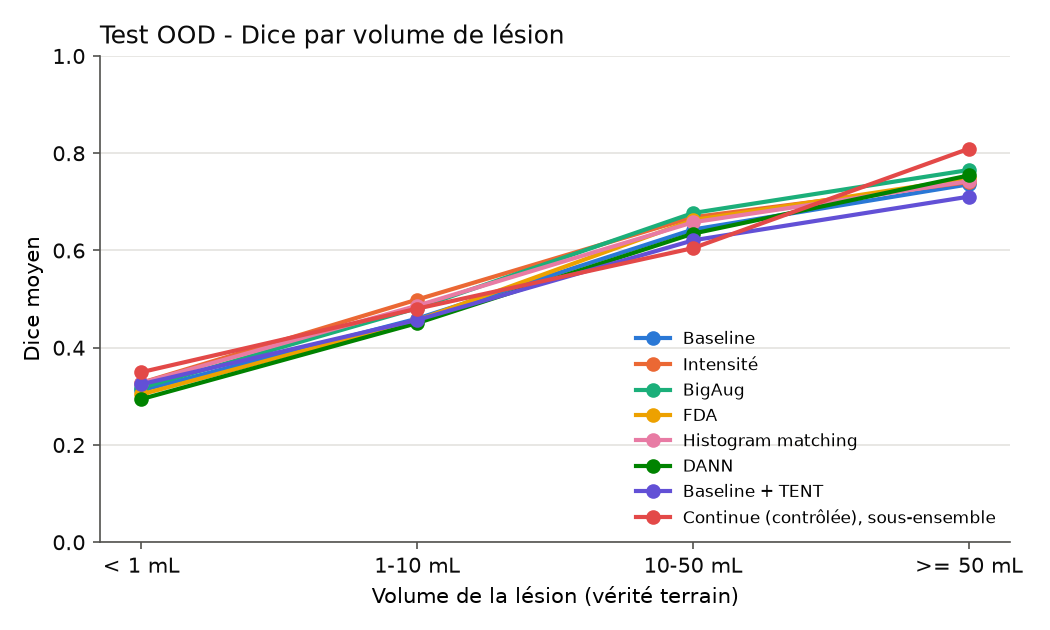
\includegraphics[width=0.8\linewidth]{figures/rq3/rq3_echecs_dice_par_taille.png}
  \caption{Dice moyen par volume de lésion sur le test OOD, avec l'adaptation continue contrôlée (sous-ensemble préquentiel).}
  \label{fig:rq3-echecs-taille}
\end{figure}

\subsection{Centre R008}

Toutes les techniques obtiennent un Dice nul ou presque sur R008. Le Dice moyen de BigAug est de 0,006 sur le centre ; un seul sujet est non nul, à 0,04 (tableau~\ref{tab:rq3-bigaug-intensite} ; moyenne arrondie à 0,01 dans le tableau~\ref{tab:rq3-centres}). Celui d'histogram matching est de 0,019, avec un seul sujet non nul, à 0,13 (tableau~\ref{tab:rq3-hm-intensite}). Le détail par sujet est dans \nolinkurl{zoom_R008_R053.csv}.
\begin{itemize}
  \item Six sujets sur sept sont imagés au premier jour après l'AVC. Leurs lésions font de 0,1 à 4,1~ml.
  \item Les lésions sont peu visibles en T1 : contraste médian de $-0{,}17$, contre $-0{,}50$ à $-0{,}98$ dans les autres centres OOD.
  \item Les intensités sont atypiques : 1,1 à 1,7~\% des voxels du cerveau dépassent $z = 3$, contre 0,003~\% en médiane chez les autres sujets OOD (\nolinkurl{contraste_lesions.csv}).
  \item Le modèle prédit de 0,4 à 33,6~ml répartis en nombreuses composantes, pour une différence du nombre de lésions de 9 à 67.
  \item À l'examen des coupes, vaisseaux, sinus et dure-mère apparaissent hyperintenses.
\end{itemize}
% Les coupes de R008 (figures/rq3/rq3_echecs_coupes_R008.png) ne sont pas incluses :
% ce sont des images ATLAS, non versionnées ; elles se régénèrent avec adaptation/analyse_echecs.py.

\emph{Hypothèse.} La séquence T1 de R008 aurait été acquise après injection de gadolinium, en phase aiguë.
La lésion n'y aurait pas encore le contraste T1 des lésions chroniques, majoritaires à l'entraînement.
Le décalage serait alors à la fois d'acquisition et de stade clinique.
Cette hypothèse reste à vérifier sur le protocole d'acquisition de R008 et sur l'écart entre la date de l'IRM et celle de l'annotation.

\subsection{Centre R053}

Le Dice moyen de R053 est de 0,20 sur quatre sujets ; un cinquième sujet a un masque vide et est exclu du Dice.
Deux lésions minuscules (0,13 et 0,015~ml) ont un Dice de 0. Les deux autres (1,5 et 2,6~ml) obtiennent 0,27 et 0,52.
Les intensités sont dans la norme (99\textsuperscript{e} centile du z-score proche de 1,8) et le contraste vaut $-0{,}50$.
L'échec s'explique par la taille des lésions, pas par un décalage d'intensité. Avec quatre sujets, la moyenne du centre est très instable.

\subsection{Distance de domaine}

La distance de Wasserstein entre histogrammes d'intensité (\nolinkurl{analysis/center_distance.py}, référence = tous les autres centres) ne prédit pas le Dice dans nos runs (\nolinkurl{spearman.csv}).
\begin{itemize}
  \item Sur les six centres OOD, $\rho$ va de $-0{,}43$ à $-0{,}03$ selon la technique ($p$ de 0,40 à 0,96). Avec la MMD, $\rho$ va de $-0{,}37$ à $-0{,}09$.
  \item Sur les 44 centres de test (ID et OOD), $\rho$ va de 0,03 à 0,12 ($p \geq 0{,}44$).
\end{itemize}
La figure~\ref{fig:rq3-distance} en donne deux contre-exemples. R053 est l'un des centres les plus proches (0,020) et l'un des pires. R031 est éloigné (0,164) et parmi les meilleurs.
Six centres offrent une puissance très faible : nous ne concluons pas à l'absence de lien, seulement qu'il n'apparaît pas ici.

\begin{figure}[htbp]
  \centering
  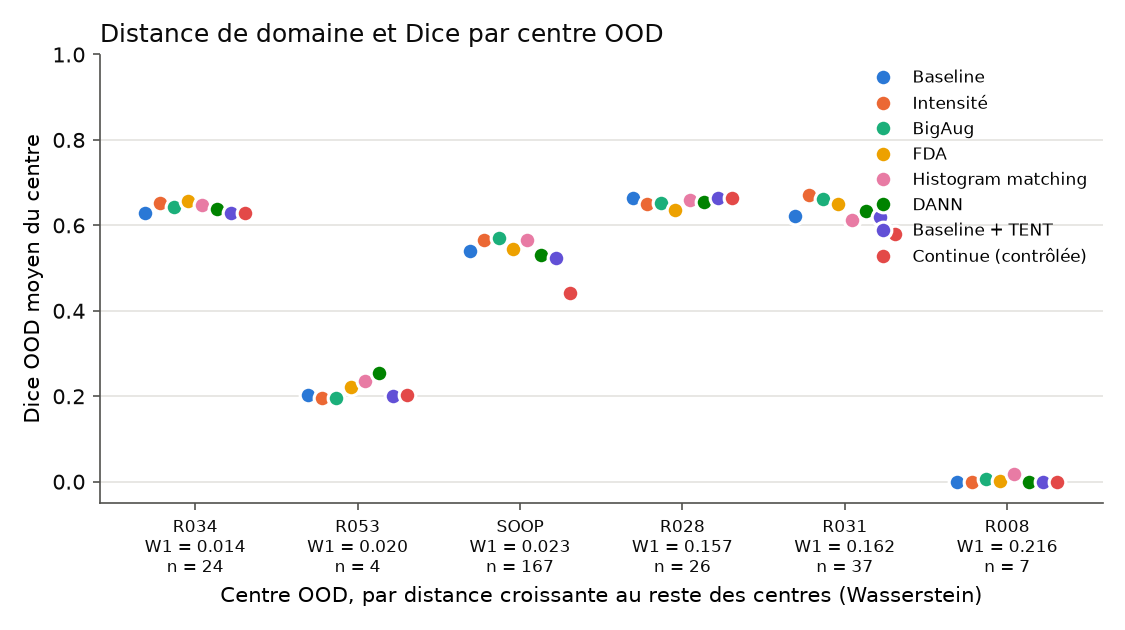
\includegraphics[width=0.8\linewidth]{figures/rq3/rq3_echecs_distance_dice.png}
  \caption{Dice OOD moyen par centre, les centres étant rangés par distance croissante au reste des centres.}
  \label{fig:rq3-distance}
\end{figure}

Au niveau des sujets, le contraste de la lésion n'est que faiblement lié au Dice ($\rho = -0{,}19$, $p = 0{,}001$). La figure~\ref{fig:rq3-contraste} montre ce nuage et place les sujets de R008 et R053.

\begin{figure}[htbp]
  \centering
  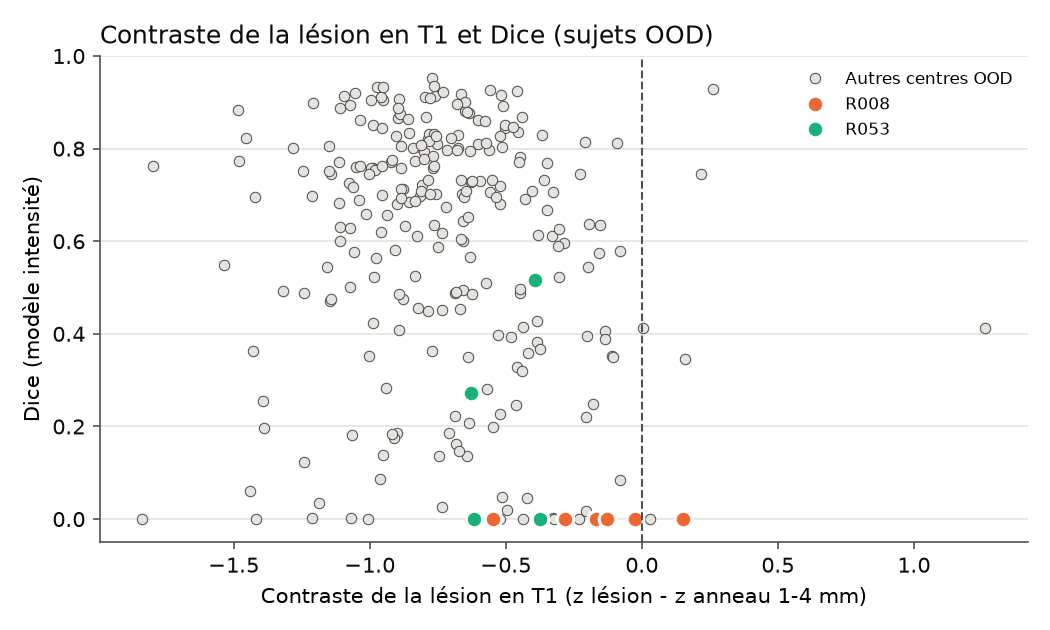
\includegraphics[width=0.8\linewidth]{figures/rq3/rq3_echecs_contraste_dice.png}
  \caption{Contraste T1 de la lésion et Dice (modèle intensité) pour les sujets OOD ; R008 et R053 sont mis en évidence.}
  \label{fig:rq3-contraste}
\end{figure}

\section{Adaptation continue contrôlée}
\label{sec:rq3-continue}

\paragraph{Protocole.}
L'expérience est réalisée par le script \nolinkurl{adaptation/continual.py}.
Ses sorties se trouvent dans le dossier \nolinkurl{adaptation/outputs/rq3/adaptation_continue/}.
Le modèle baseline reçoit les six centres OOD l'un après l'autre, par lots de quatre sujets : 28 lots, 108 sujets, au plus 24 par centre. Il n'est jamais réinitialisé.
L'évaluation est préquentielle : chaque lot est d'abord noté (Dice), puis utilisé pour l'adaptation, sans étiquettes.
Quatre stratégies sont comparées sur les mêmes lots :
\begin{itemize}
  \item \texttt{fige} : le modèle reste inchangé ;
  \item \texttt{auto\_apprentissage} : pseudo-étiquettes, tous les poids sont mis à jour ;
  \item \texttt{tent} : TENT appliqué en continu ;
  \item \texttt{controlee} : TENT dans un modèle candidat, promu seulement si trois conditions sont réunies. (1) La distance du lot dépasse un seuil calibré sur la source (0,077). (2) L'entropie baisse sur des patches neufs. (3) Le Dice sur un jeu de garde étiqueté de la source ne baisse pas de plus de 0,01. Cette stratégie rejoue aussi des exemples des centres déjà vus et des patches de la source.
\end{itemize}
L'oubli est mesuré après chaque centre, par le Dice sur 16 sujets fixes du test ID et sur les premiers sujets des centres OOD déjà vus.

\paragraph{Résultats.}
Le tableau~\ref{tab:rq3-continue} résume les quatre stratégies (\nolinkurl{resume.json}, \nolinkurl{oubli.csv}).

\begin{table}[htbp]
  \centering
  \caption{Adaptation continue sur les six centres OOD : Dice préquentiel et oubli.}
  \label{tab:rq3-continue}
  \small
  \begin{tabular}{lcccc}
    \toprule
    Stratégie & \makecell{Dice\\préquentiel} & \makecell{Dice ID\\(début $\rightarrow$ fin)} & Oubli ID & \makecell{Oubli OOD\\moyen} \\
    \midrule
    Figé & 0,528 & 0,635 $\rightarrow$ 0,635 & 0,000 & 0,000 \\
    Auto-apprentissage & 0,486 & 0,635 $\rightarrow$ 0,583 & 0,052 & 0,033 \\
    TENT continu & 0,526 & 0,635 $\rightarrow$ 0,632 & 0,002 & 0,000 \\
    Contrôlée & 0,527 & 0,635 $\rightarrow$ 0,634 & 0,001 & 0,000 \\
    \bottomrule
  \end{tabular}
\end{table}

Les décisions lot par lot sont dans \nolinkurl{decisions.csv}.
\begin{itemize}
  \item \textbf{Détection.} Un décalage est détecté sur 15 lots sur 28 : tous ceux de R008, R028 et R031, et un lot sur six de SOOP. Il n'est jamais détecté sur R034 ni R053, les centres les plus proches de la source.
  \item \textbf{Promotions.} Douze candidats sont promus : deux pour R008, six pour R028, trois pour R031 et un pour SOOP. Trois candidats de R031 sont refusés parce que leur entropie augmente.
  \item \textbf{Oubli.} La stratégie contrôlée évite l'oubli de l'auto-apprentissage (0,001 contre 0,052 sur le test ID).
  \item \textbf{Gain.} Elle n'améliore pas le Dice par rapport au modèle figé (0,527 contre 0,528).
\end{itemize}

\paragraph{Lecture du résultat.}
L'absence de gain s'explique par la nature des décalages détectés.
R028 et R031 sont déjà bien segmentés par le modèle figé (0,66 et 0,58 en préquentiel).
Sur R008, le problème tient au contraste des lésions (section~\ref{sec:rq3-echecs}), qu'une adaptation des normalisations ne peut pas créer.
Les Dice préquentiels portent sur 108 des 268 sujets OOD ; ils ne se comparent pas directement au tableau~\ref{tab:rq3-resultats}.

\section{Limites}
\label{sec:rq3-limites}

\begin{itemize}
  \item \textbf{Un seul pli et une seule graine.} Les IC traduisent la variabilité des sujets, pas celle de l'entraînement.
  \item \textbf{Reprise de DANN.} La run a été coupée à l'itération 35\,889 et reprise jusqu'à 40\,000. La reprise restaure les poids, l'optimiseur, le taux d'apprentissage, $\lambda$, la position de l'échantillonneur et les états aléatoires des processus de chargement. Le contrôle automatique a validé la première ligne reprise (itération 35\,900, taux $1{,}29 \times 10^{-4}$, $\lambda = 0{,}9771$). Seuls les masques de Dropout du classifieur de centre ne sont pas restaurés. Le meilleur modèle, à l'itération 24\,000, précède de toute façon la coupure.
  \item \textbf{Environnement de DANN.} DANN a été entraînée sur Colab avec torch 2.14.1+cu130 jusqu'à l'itération 35\,889, puis sur Kaggle avec torch 2.11.0+cu130, comme les autres runs. Les deux plateformes utilisent un GPU T4 et CUDA 13.0. Le meilleur modèle (itération 24\,000) vient de la partie Colab. La différence de version de torch peut changer les calculs numériques ; son effet n'a pas été mesuré.
  \item \textbf{Poids de DANN.} Avec un poids de 1, la première run DANN a divergé (perte totale de 10\,508 à l'itération 100 et de 33 millions à l'itération 400). Le poids de 0,1 et la LayerNorm ont été choisis pour la stabilité, sans recherche d'hyperparamètres. Un autre poids pourrait donner un autre résultat.
  \item \textbf{Validation sur des centres non vus.} Ses lésions sont plus petites que celles du test. Elle sert à choisir le checkpoint, mais son Dice (environ 0,43) n'estime pas la performance ID.
  \item \textbf{Diagnostic fp16.} La première baseline, entraînée en fp16, a produit des NaN : des patches entiers donnaient des logits NaN dès l'itération 160 à 180 environ, alors que le fp32 restait stable sur les mêmes lots. Toutes les runs ont été refaites en fp32, environ deux fois plus lentement. La couche qui déborde n'a pas été localisée.
  \item \textbf{Bug de reprise corrigé.} Dans la version du code utilisée pour les runs, la ligne de progression écrasait la file des états aléatoires sauvegardés pour la reprise. Le défaut ne concerne que les reprises, donc uniquement DANN. Il a été corrigé et couvert par un test. Le checkpoint de DANN a été réparé avant la reprise en ne gardant que les quatre derniers états, qui étaient les bons ; les poids n'ont pas changé.
  \item \textbf{Référence de la distance de domaine.} Pour chaque centre, la référence de \nolinkurl{center_distance} regroupe tous les autres centres, OOD compris, et pas seulement les centres d'entraînement du pli~0. La distance mesure donc l'écart au reste du jeu de données, pas exactement l'écart à ce que le modèle a vu.
  \item \textbf{Version du code d'histogram matching.} Cette run a utilisé une version ultérieure du code (\texttt{dbf2f28} au lieu de \texttt{7449c49}), qui ne diffère que par la correction du bug de reprise. Sans DANN ni reprise, les deux versions donnent des poids identiques (vérifié par un court entraînement sur CPU, pour la baseline et l'intensité).
  \item \textbf{Quota GPU.} Avec 30~h par semaine sur Kaggle, aucun autre pli n'a été entraîné, et l'histogram matching a été lancé après les autres techniques.
  \item \textbf{Portée de TENT et de l'adaptation continue.} Les deux ne sont évalués que sur la baseline.
\end{itemize}

\section{Conclusion}
\label{sec:rq3-conclusion}

Sur le pli~0, seule l'augmentation d'intensité améliore le Dice OOD de façon significative après correction : $+0{,}024$ [0,008 ; 0,041], $p$ Holm $= 0{,}0068$ (tableau~\ref{tab:rq3-resultats}).
BigAug atteint le même Dice OOD (0,577), mais son gain n'est pas significatif après correction ($p$ Holm $= 0{,}14$), et la comparaison directe ne sépare pas les deux techniques ($+0{,}001$ [$-0{,}010$ ; 0,012], tableau~\ref{tab:rq3-bigaug-intensite}).
Histogram matching n'est pas significatif non plus ($+0{,}017$, $p$ Holm $= 0{,}49$) ; il reste en dessous de l'intensité en Dice OOD ($-0{,}007$ [$-0{,}023$ ; 0,009]), avec un écart net sur R031 (tableau~\ref{tab:rq3-hm-intensite}).
Aucune technique ne supprime l'écart ID $-$ OOD, qui reste compris entre 0,075 et 0,104.
FDA, DANN et TENT n'améliorent pas le test OOD ; TENT le dégrade légèrement.
L'adaptation continue contrôlée évite l'oubli sans améliorer le Dice (tableau~\ref{tab:rq3-continue}).
L'analyse des échecs montre que les cas les plus difficiles tiennent aux lésions elles-mêmes, petites ou peu contrastées en T1, plutôt qu'à la distance d'intensité entre centres.
Le livrable C8 (\nolinkurl{adaptation/inference.py}) segmente un T1 et renvoie le masque et le volume de la lésion.
Le modèle retenu pour la démonstration est celui de l'intensité.
À Dice égal avec BigAug, ce choix repose d'abord sur son gain significatif après correction, ensuite sur un entraînement plus court (5,0~h contre 8,1~h).
Son F1 des lésions est supérieur à celui de BigAug (0,450 contre 0,420) mais inférieur à celui de la baseline (0,477) : ce n'est qu'un argument relatif face à BigAug.
Histogram matching a le plus faible écart absolu de volume (9,1~ml contre 10,0~ml pour l'intensité) et un F1 des lésions supérieur à celui de la baseline (0,486 contre 0,477).
Il n'a pas été retenu, car son gain en Dice n'est pas significatif et il exigerait d'harmoniser aussi chaque volume à l'inférence, avec l'histogramme de référence de R059.
Ces constats orientent la suite vers la prédiction des cas à risque, en particulier les lésions de moins de 1~ml et les AVC en phase aiguë.
.
% Paquets attendus dans le préambule : babel (french), graphicx, booktabs, makecell, hyperref, float.
% Réglages à mettre dans le préambule du rapport final :
%   \addto\captionsfrench{\def\tablename{Tableau}}   % « Tableau » au lieu de « Table »
%   \hypersetup{hidelinks}                             % liens sans cadre rouge
% Les chemins des figures sont relatifs à la racine du dépôt.
% Citations : docs/rapport/references_rq3.bib, à ajouter à la commande \bibliography du rapport.

\chapter{Généralisation inter-centres (RQ3) et adaptation continue contrôlée}
\label{chap:rq3}

\section{Introduction}
\label{sec:rq3-introduction}

Ce chapitre étudie la robustesse d'un modèle de segmentation des lésions d'AVC face à des centres d'acquisition jamais vus.
La question de recherche RQ3 est la suivante : « Quelles techniques de data augmentation et/ou d'adaptation de domaine réduisent le plus efficacement l'écart de performance entre centres ? »
Nous mesurons cet écart entre des centres vus à l'entraînement (ID) et des centres non vus (OOD).
Nous décrivons d'abord le protocole et les techniques évaluées, puis les résultats et l'analyse des échecs.
Nous présentons ensuite une adaptation continue contrôlée, avant de discuter les limites de l'étude.

\section{Protocole expérimental}
\label{sec:rq3-protocole}

\paragraph{Données.}
Nous utilisons les images T1 d'ATLAS v2.0~\cite{liew2022atlas}, déjà débarrassées du crâne, après le prétraitement S4 de l'équipe : orientation RAS, rééchantillonnage à 1~mm, recadrage sur le cerveau et z-score dans le cerveau (\nolinkurl{preprocessing/week4.py}).
Le découpage est fixé dans \nolinkurl{splits.json}. Le centre R032 est exclu.

\paragraph{Découpage par centre.}
Six centres sont réservés au test OOD : R008, R028, R031, R034, R053 et SOOP.
Ils ont été choisis sur la taille des centres et la distance entre histogrammes d'intensité, sans consulter le Dice (champ \texttt{selection} de \nolinkurl{splits.json}).
Les autres centres sont répartis en cinq plis. Seul le pli~0 a été entraîné. Le tableau~\ref{tab:rq3-donnees} donne les effectifs.

\begin{table}[htbp]
  \centering
  \caption{Effectifs du pli~0.}
  \label{tab:rq3-donnees}
  \begin{tabular}{lrl}
    \toprule
    Ensemble & Sujets & Centres \\
    \midrule
    Entraînement & 733 & 39 \\
    Validation & 183 & 9 centres absents de l'entraînement \\
    Test ID & 185 & centres d'entraînement, sujets non vus \\
    Test OOD & 268 (265 à lésion non vide) & 6 \\
    \bottomrule
  \end{tabular}
\end{table}

Le découpage de \nolinkurl{splits.json} compte 184 sujets de validation.
L'un d'eux, le sujet r065s019 du centre R065, n'a pas de volume prétraité.
Le prétraitement S4 l'a rejeté, car une partie de sa lésion sort du recadrage calculé sur l'image.
Le chargeur l'écarte, et la validation porte donc sur 183 sujets, comme l'indiquent les journaux d'entraînement.
Un de ces 183 sujets a un masque vide : le Dice de validation est calculé sur 182 sujets.

\paragraph{Modèle et entraînement.}
Le réseau est un U-Net~3D de MONAI~\cite{cardoso2022monai} : canaux de 32 à 320, quatre sous-échantillonnages et deux unités résiduelles par niveau.
La normalisation d'instance est affine, ce qu'exige TENT.
L'entraînement utilise des patches de $96^3$ voxels, par lots de quatre patches (deux volumes $\times$ deux patches), dont la moitié est centrée sur la lésion.
Un miroir gauche-droite aléatoire est appliqué à toutes les runs.
La perte combine Dice et entropie croisée.
L'optimiseur AdamW part d'un taux d'apprentissage de $10^{-3}$, avec une décroissance polynomiale (puissance 0,9) et une décroissance des poids de $10^{-5}$.
La norme des gradients est écrêtée à 12.
Toutes les techniques reçoivent le même budget : 40\,000 itérations, graine 2026, calcul en fp32 sur un GPU T4.
Les runs ont été exécutées sur Kaggle (torch 2.11.0+cu130), sauf DANN.
DANN a été entraînée sur Google Colab (GPU T4, torch 2.14.1+cu130) jusqu'à l'itération 35\,889, puis reprise sur Kaggle jusqu'à 40\,000 (section~\ref{sec:rq3-limites}).

\paragraph{Sélection du modèle.}
Le modèle est validé toutes les 2\,000 itérations sur les 183 sujets de validation, en volume entier, par fenêtre glissante de $96^3$ (recouvrement 0,25).
Le checkpoint retenu est celui du meilleur Dice de validation. Il est évalué une seule fois sur les tests ID et OOD.

\paragraph{Métriques.}
Nous rapportons le Dice, la distance de Hausdorff à 95~\% (HD95), l'écart absolu de volume, le F1 des lésions et la différence du nombre de lésions.
Ces métriques sont communes à l'équipe (\nolinkurl{baselines/common.py}).
Le Dice n'est calculé que sur les sujets dont la lésion n'est pas vide.

\paragraph{Tests statistiques.}
Les moyennes sont données avec un intervalle de confiance (IC) à 95~\% par bootstrap percentile (10\,000 tirages).
Pour l'écart ID $-$ OOD, les deux groupes sont rééchantillonnés indépendamment.
Chaque technique est comparée à la baseline par un test des rangs signés de Wilcoxon~\cite{wilcoxon1945}, apparié sur les mêmes sujets.
Une correction de Holm~\cite{holm1979} est appliquée sur l'ensemble des techniques comparées.
La correction porte sur six comparaisons : intensité, BigAug, FDA, histogram matching, DANN et TENT.
BigAug et histogram matching sont aussi comparés directement à l'intensité (différence appariée, IC bootstrap, Wilcoxon), hors correction de Holm : ce sont des comparaisons secondaires avec la technique de référence.

\section{Techniques évaluées}
\label{sec:rq3-techniques}

Toutes les techniques partagent le réseau, les plis, les graines et le budget d'itérations. Seule l'étape propre à chaque technique change (\nolinkurl{adaptation/train.py}, \nolinkurl{generalization/configs/}).

\begin{itemize}
  \item \textbf{Augmentation d'intensité.} Gamma ($p = 0{,}3$) et contraste ($p = 0{,}3$), calibrés sur les seuls sujets d'entraînement ; bruit ($p = 0{,}2$), flou ($p = 0{,}2$), champ de biais ($p = 0{,}3$) et basse résolution ($p = 0{,}25$, jusqu'à 3~mm sur un axe).
  \item \textbf{BigAug}~\cite{zhang2020bigaug}. Flou, netteté, bruit, luminosité, gamma (plage calibrée) et transformation affine (échelle de 0,8 à 1,2, rotation de 20\textdegree), chacun avec $p = 0{,}5$. La déformation élastique est désactivée. Les plages sont adoucies par rapport à l'article pour préserver les petites lésions.
  \item \textbf{FDA} (Fourier Domain Adaptation)~\cite{yang2020fda}. L'amplitude basse fréquence est échangée avec celle d'une image d'un centre d'entraînement de référence (R059 pour le pli~0), avec $\beta$ entre 0,015 et 0,03 et $p = 0{,}5$.
  \item \textbf{DANN} (Domain-Adversarial Neural Network)~\cite{ganin2016dann}. Un classifieur des 39 centres d'entraînement est branché sur la sortie du goulot du réseau : moyenne spatiale, LayerNorm sans paramètres, puis perceptron de 64 unités. Une couche d'inversion du gradient le relie à l'encodeur. Le coefficient $\lambda$ est nul pendant les 2\,000 premières itérations, puis suit la montée proposée par Ganin et al.\ ($\gamma = 5$). La perte du centre a un poids de 0,1.
  \item \textbf{TENT}~\cite{wang2021tent}. Adaptation au test, sans étiquettes, du modèle baseline. Seuls les paramètres affines des normalisations sont modifiés, en minimisant l'entropie des prédictions, centre par centre (Adam, taux de $10^{-4}$, quatre patches par sujet).
  \item \textbf{Histogram matching.} L'histogramme d'intensité du cerveau de chaque volume est ramené vers un histogramme de référence, moyenné sur 20 sujets d'un centre d'entraînement (R059 pour le pli~0). La transformation est déterministe ($p = 1$) et s'applique aussi à la validation et au test. Faute de quota GPU, cette run a été lancée après les autres, avec une version ultérieure du code (section~\ref{sec:rq3-limites}).
\end{itemize}
Fan-Net~\cite{yu2023fannet} n'a pas été implémenté ; FDA en reprend le principe (échange d'amplitude de Fourier) sous une forme plus simple.

\section{Résultats RQ3}
\label{sec:rq3-resultats}

Le tableau~\ref{tab:rq3-resultats} résume les résultats sur 185 sujets ID et 265 sujets OOD (\nolinkurl{adaptation/outputs/rq3/tableau_rq3.md}).

\begin{table}[htbp]
  \centering
  \caption{Dice moyen par technique (pli~0), avec l'IC à 95~\% sous chaque valeur. $\Delta$ OOD : différence appariée à la baseline sur le test OOD ; $p$ : test de Wilcoxon, puis $p$ corrigé par Holm.}
  \label{tab:rq3-resultats}
  \small
  \setlength{\tabcolsep}{4pt}
  \begin{tabular}{lccccc}
    \toprule
    Technique & Dice ID & Dice OOD & \makecell{Écart\\ID $-$ OOD} & $\Delta$ OOD & $p$ OOD \\
    \midrule
    Baseline & \makecell{0,646\\{\footnotesize [0,611 ; 0,680]}} & \makecell{0,553\\{\footnotesize [0,517 ; 0,589]}} & \makecell{0,093\\{\footnotesize [0,044 ; 0,142]}} & -- & -- \\[2pt]
    Intensité & \makecell{0,656\\{\footnotesize [0,621 ; 0,690]}} & \makecell{0,577\\{\footnotesize [0,543 ; 0,611]}} & \makecell{0,080\\{\footnotesize [0,031 ; 0,126]}} & \makecell{+0,024\\{\footnotesize [0,008 ; 0,041]}} & \makecell{0,0014\\{\footnotesize (Holm 0,0068)}} \\[2pt]
    BigAug & \makecell{0,653\\{\footnotesize [0,619 ; 0,686]}} & \makecell{0,577\\{\footnotesize [0,543 ; 0,611]}} & \makecell{0,075\\{\footnotesize [0,028 ; 0,122]}} & \makecell{+0,025\\{\footnotesize [0,010 ; 0,040]}} & \makecell{0,035\\{\footnotesize (Holm 0,14)}} \\[2pt]
    FDA & \makecell{0,660\\{\footnotesize [0,626 ; 0,693]}} & \makecell{0,559\\{\footnotesize [0,524 ; 0,593]}} & \makecell{0,101\\{\footnotesize [0,053 ; 0,148]}} & \makecell{+0,006\\{\footnotesize [$-$0,007 ; 0,020]}} & \makecell{0,32\\{\footnotesize (Holm 0,49)}} \\[2pt]
    \makecell[l]{Histogram\\matching} & \makecell{0,646\\{\footnotesize [0,611 ; 0,681]}} & \makecell{0,570\\{\footnotesize [0,536 ; 0,604]}} & \makecell{0,077\\{\footnotesize [0,027 ; 0,125]}} & \makecell{+0,017\\{\footnotesize [0,001 ; 0,034]}} & \makecell{0,24\\{\footnotesize (Holm 0,49)}} \\[2pt]
    DANN & \makecell{0,650\\{\footnotesize [0,616 ; 0,684]}} & \makecell{0,549\\{\footnotesize [0,513 ; 0,584]}} & \makecell{0,102\\{\footnotesize [0,053 ; 0,150]}} & \makecell{$-$0,004\\{\footnotesize [$-$0,018 ; 0,009]}} & \makecell{0,13\\{\footnotesize (Holm 0,39)}} \\[2pt]
    \makecell[l]{Baseline\\+ TENT} & \makecell{0,645\\{\footnotesize [0,610 ; 0,679]}} & \makecell{0,542\\{\footnotesize [0,506 ; 0,578]}} & \makecell{0,104\\{\footnotesize [0,054 ; 0,153]}} & \makecell{$-$0,011\\{\footnotesize [$-$0,016 ; $-$0,006]}} & \makecell{$< 10^{-4}$\\{\footnotesize (Holm $< 10^{-4}$)}} \\[2pt]
    \bottomrule
  \end{tabular}
\end{table}

La figure~\ref{fig:rq3-dice-id-ood} montre les Dice ID et OOD de chaque technique avec leurs IC.
L'écart entre ID et OOD demeure pour toutes les techniques : il va de 0,075 à 0,104, et aucun IC ne contient 0.

\begin{figure}[htbp]
  \centering
  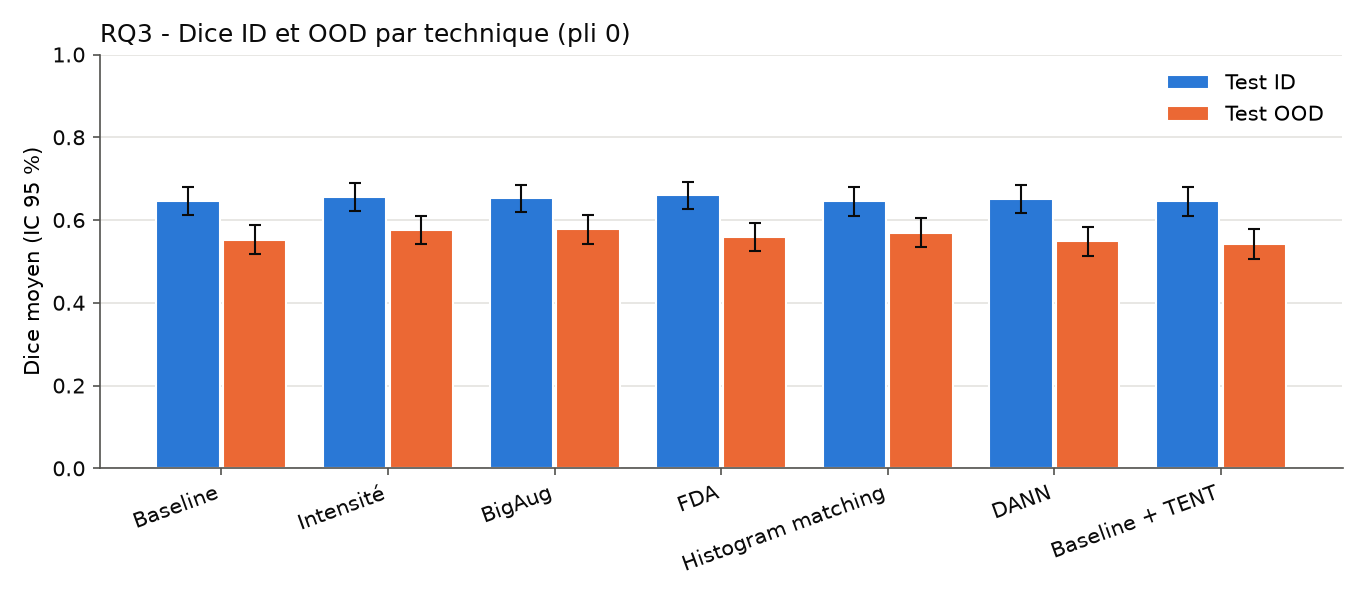
\includegraphics[width=0.8\linewidth]{figures/rq3/rq3_dice_id_ood.png}
  \caption{Dice moyen sur les tests ID et OOD par technique, avec IC à 95~\% (pli~0).}
  \label{fig:rq3-dice-id-ood}
\end{figure}

La figure~\ref{fig:rq3-delta-ood} montre la distribution des différences appariées à la baseline sur le test OOD.
\begin{itemize}
  \item L'augmentation d'intensité est la seule technique qui améliore le Dice OOD de façon significative après correction : $+0{,}024$ [0,008 ; 0,041], $p = 0{,}0014$, $p$ Holm $= 0{,}0068$. Le gain est réparti : 155 sujets sur 252 différences non nulles sont en sa faveur, pour une médiane de $+0{,}006$.
  \item BigAug obtient le même gain moyen ($+0{,}025$ [0,010 ; 0,040]), mais son Wilcoxon ($p = 0{,}035$) n'est plus significatif après correction ($p$ Holm $= 0{,}14$). La différence médiane avec la baseline est quasi nulle ($+0{,}001$ ; 135 sujets en sa faveur sur 250 différences non nulles), et la moyenne est tirée par quelques grands écarts, jusqu'à $+0{,}67$. C'est ce qui explique que le Wilcoxon, fondé sur les rangs, ne passe pas la correction de Holm. Son écart ID $-$ OOD est le plus faible (0,075), mais son IC chevauche celui de la baseline.
  \item FDA a le meilleur Dice ID (0,660), mais son gain sur la baseline n'est significatif après correction ni en ID (Wilcoxon $p = 0{,}012$, $p$ Holm $= 0{,}061$ ; $\Delta$ ID $= +0{,}014$ [$-$0,001 ; 0,029]), ni en OOD ($p = 0{,}32$).
  Avant correction, le Wilcoxon en ID est significatif alors que l'IC bootstrap de $\Delta$ ID contient 0, car les deux ne testent pas la même chose.
  Le Wilcoxon porte sur les rangs des différences appariées : 109 sujets sur 179 différences non nulles sont en faveur de FDA, pour une médiane de $+0{,}005$.
  L'IC porte sur la moyenne, que quelques grandes différences dans les deux sens (jusqu'à $-0{,}32$) rendent plus variable.
  \item Histogram matching améliore le Dice OOD en moyenne ($+0{,}017$ [0,001 ; 0,034]), mais pas de façon significative ($p = 0{,}24$, $p$ Holm $= 0{,}49$). L'IC bootstrap de $\Delta$ OOD exclut tout juste 0 alors que le Wilcoxon n'est pas significatif, pour la même raison que FDA en ID : l'IC porte sur la moyenne, tirée par quelques grands écarts (jusqu'à $+0{,}84$), et le Wilcoxon sur les rangs, avec une médiane nulle (125 sujets en sa faveur, 125 en sa défaveur). Son écart ID $-$ OOD (0,077) est proche de celui de BigAug.
  \item DANN ne se distingue de la baseline ni en ID ($p = 0{,}45$) ni en OOD ($p = 0{,}13$).
  \item TENT abaisse le Dice OOD de 0,011 [0,006 ; 0,016]. L'effet est petit mais systématique ($p < 10^{-4}$). En ID, la baisse est de 0,0007 [0,0002 ; 0,0012] ($p = 1{,}7 \times 10^{-4}$, $p$ Holm $= 1{,}0 \times 10^{-3}$).
\end{itemize}

\begin{figure}[htbp]
  \centering
  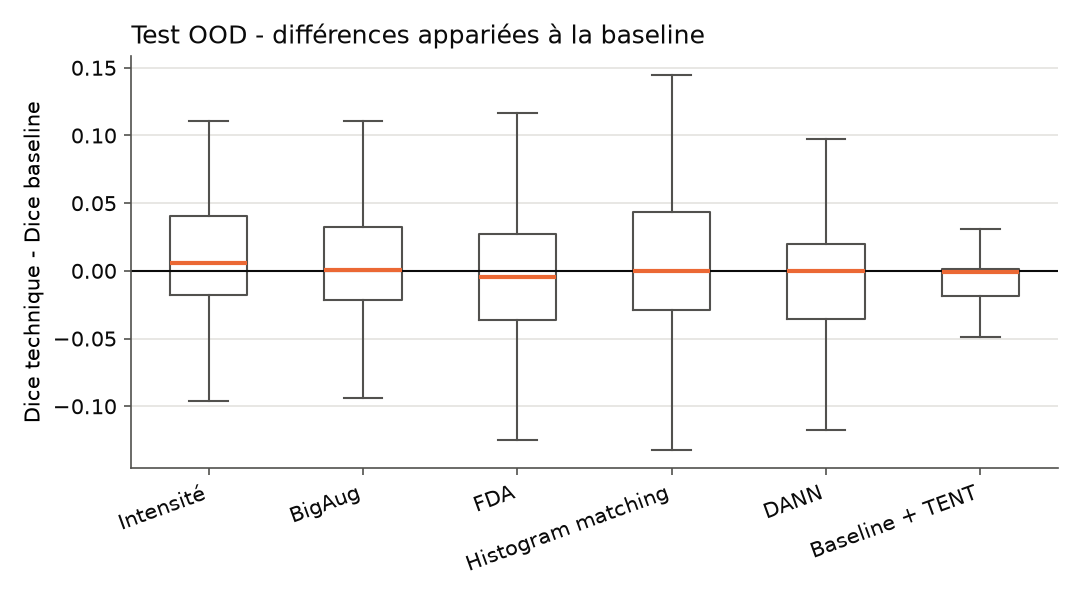
\includegraphics[width=0.8\linewidth]{figures/rq3/rq3_delta_ood.png}
  \caption{Différences appariées de Dice avec la baseline, par sujet, sur le test OOD.}
  \label{fig:rq3-delta-ood}
\end{figure}

\paragraph{BigAug et intensité.}
Le tableau~\ref{tab:rq3-bigaug-intensite} compare directement les deux techniques sur les mêmes sujets (\nolinkurl{adaptation/outputs/rq3/comparaisons.csv}).
Sur le test OOD, la différence moyenne BigAug $-$ intensité vaut $+0{,}001$ [$-0{,}010$ ; 0,012] ($p = 0{,}53$ ; 123 sujets en faveur de BigAug, 128 en faveur de l'intensité).
Sur le test ID, elle vaut $-0{,}003$ [$-0{,}017$ ; 0,011] ($p = 0{,}35$).
Aucun centre OOD ne les sépare : les différences vont de $-0{,}011$ (R034) à $+0{,}006$ (R008), toutes avec $p \geq 0{,}32$.
Les deux techniques sont donc équivalentes en Dice à la précision de cette étude.
Elles diffèrent sur deux points secondaires.
L'entraînement de BigAug dure 8,1~h contre 5,0~h pour l'intensité (\nolinkurl{adaptation/outputs/rq3/entrainement.csv}).
Le F1 des lésions OOD est plus élevé avec l'intensité qu'avec BigAug (0,450 contre 0,420), mais les deux restent sous la baseline (0,477, tableau~\ref{tab:rq3-secondaires}) : ce n'est qu'un avantage relatif face à BigAug.

\begin{table}[htbp]
  \centering
  \caption{Comparaison directe BigAug $-$ intensité par centre OOD (sujets appariés). Source : \texttt{comparaisons\_par\_centre.csv}.}
  \label{tab:rq3-bigaug-intensite}
  \small
  \setlength{\tabcolsep}{4pt}
  \begin{tabular}{lcccccc}
    \toprule
    Centre & n & Dice BigAug & Dice intensité & $\Delta$ moyen & \makecell{Sujets\\BigAug > / < intensité} & $p$ Wilcoxon \\
    \midrule
    R008 & 7 & 0,006 & 0,000 & +0,006 & 1 / 0 & 1 \\
    R028 & 26 & 0,652 & 0,649 & +0,003 & 16 / 10 & 0,50 \\
    R031 & 37 & 0,663 & 0,672 & $-$0,009 & 15 / 22 & 0,32 \\
    R034 & 24 & 0,642 & 0,653 & $-$0,011 & 11 / 12 & 0,76 \\
    R053 & 4 & 0,195 & 0,197 & $-$0,002 & 1 / 1 & 1 \\
    SOOP & 167 & 0,571 & 0,567 & +0,004 & 79 / 83 & 0,60 \\
    \midrule
    Total OOD & 265 & 0,577 & 0,577 & +0,001 & 123 / 128 & 0,53 \\
    \bottomrule
  \end{tabular}
\end{table}

\paragraph{Histogram matching et intensité.}
Le tableau~\ref{tab:rq3-hm-intensite} compare de la même façon histogram matching et intensité.
Sur le test OOD, la différence moyenne histogram matching $-$ intensité vaut $-0{,}007$ [$-0{,}023$ ; 0,009] ($p = 0{,}062$ ; 110 sujets en faveur d'histogram matching, 142 en faveur de l'intensité).
Sur le test ID, elle vaut $-0{,}010$ [$-0{,}025$ ; 0,005] ($p = 0{,}35$).
Le seul écart net par centre concerne R031 : $-0{,}059$ ($p = 0{,}0018$ ; 10 sujets contre 27), qui reste sous 0,05 après une correction de Bonferroni sur les six centres.
Histogram matching a en revanche un F1 des lésions OOD supérieur à celui de la baseline (0,486 contre 0,477) et le plus faible écart absolu de volume de toutes les techniques (9,1~ml, tableau~\ref{tab:rq3-secondaires}).

\begin{table}[htbp]
  \centering
  \caption{Comparaison directe histogram matching $-$ intensité par centre OOD (sujets appariés). HM : histogram matching. Source : \texttt{comparaisons\_par\_centre.csv}.}
  \label{tab:rq3-hm-intensite}
  \small
  \setlength{\tabcolsep}{4pt}
  \begin{tabular}{lcccccc}
    \toprule
    Centre & n & Dice HM & Dice intensité & $\Delta$ moyen & \makecell{Sujets\\HM > / < intensité} & $p$ Wilcoxon \\
    \midrule
    R008 & 7 & 0,019 & 0,000 & +0,019 & 1 / 0 & 1 \\
    R028 & 26 & 0,659 & 0,649 & +0,010 & 16 / 9 & 0,23 \\
    R031 & 37 & 0,614 & 0,672 & $-$0,059 & 10 / 27 & 0,0018 \\
    R034 & 24 & 0,648 & 0,653 & $-$0,005 & 14 / 9 & 0,41 \\
    R053 & 4 & 0,237 & 0,197 & +0,040 & 1 / 1 & 1 \\
    SOOP & 167 & 0,566 & 0,567 & 0,000 & 68 / 96 & 0,11 \\
    \midrule
    Total OOD & 265 & 0,570 & 0,577 & $-$0,007 & 110 / 142 & 0,062 \\
    \bottomrule
  \end{tabular}
\end{table}

\paragraph{Lecture des résultats négatifs.}
Les résultats de DANN et de TENT ne sont pas des défaillances techniques. La run DANN est allée à son terme, avec un contrôle de reprise validé (section~\ref{sec:rq3-limites}). TENT a été appliqué au modèle baseline sur les mêmes sujets. Les deux sont évalués comme les autres techniques.
Pour DANN, l'alignement des caractéristiques entre 39 centres n'apporte rien de mesurable.
Une explication compatible avec nos données est que les échecs OOD dépendent surtout de la taille et du contraste des lésions (section~\ref{sec:rq3-echecs}), deux facteurs que l'alignement des centres ne traite pas.
Pour TENT, la minimisation de l'entropie rend les prédictions plus tranchées sans étiquettes. La baisse touche surtout les lésions de plus de 50~ml (0,71 contre 0,74, tableau~\ref{tab:rq3-taille}).

\paragraph{Métriques secondaires.}
Elles ne suivent pas toujours le Dice (tableau~\ref{tab:rq3-secondaires}).
Le F1 des lésions OOD baisse avec l'intensité (0,450 contre 0,477), BigAug (0,420), FDA et DANN (0,366 et 0,367) ; il augmente avec histogram matching (0,486) et TENT (0,495).
L'écart absolu de volume baisse surtout avec histogram matching (9,1~ml contre 11,1~ml), puis avec l'intensité (10,0~ml) et BigAug (10,9~ml).

\begin{table}[htbp]
  \centering
  \caption{Métriques secondaires moyennes sur le test OOD (\texttt{tableau\_rq3.csv}).}
  \label{tab:rq3-secondaires}
  \begin{tabular}{lccc}
    \toprule
    Technique & F1 des lésions & HD95 (mm) & Écart absolu de volume (ml) \\
    \midrule
    Baseline & 0,477 & 24,9 & 11,1 \\
    Intensité & 0,450 & 25,5 & 10,0 \\
    BigAug & 0,420 & 25,4 & 10,9 \\
    FDA & 0,366 & 26,1 & 13,3 \\
    Histogram matching & 0,486 & 24,9 & 9,1 \\
    DANN & 0,367 & 27,2 & 12,1 \\
    Baseline + TENT & 0,495 & 25,9 & 12,1 \\
    \bottomrule
  \end{tabular}
\end{table}

\paragraph{Validation et test.}
Les meilleurs Dice de validation vont de 0,427 à 0,443 (\nolinkurl{adaptation/outputs/rq3/entrainement.csv}). La validation ne départage donc pas les techniques.
Le Dice de validation (environ 0,43) est plus bas que celui du test ID (0,646) pour deux raisons.
La validation porte sur neuf centres non vus.
Ses lésions sont aussi plus petites : médiane de 1,26~ml et 43~\% sous 1~ml, contre 7,56~ml et 18~\% au test ID (volumes \texttt{lesion\_ml} des fichiers \texttt{qc.json}).

\section{Analyse des échecs}
\label{sec:rq3-echecs}

Les tableaux détaillés de cette section sont produits par le script \nolinkurl{adaptation/analyse_echecs.py}.
Ils se trouvent dans le dossier \nolinkurl{adaptation/outputs/rq3/echecs/}.

\subsection{Dice par centre OOD}

Le tableau~\ref{tab:rq3-centres} et la figure~\ref{fig:rq3-dice-centre} donnent le Dice moyen par centre.
Le contraste T1 est la différence entre le z-score moyen de la lésion et celui d'un anneau de 1 à 4~mm autour d'elle. Une lésion chronique est hypo-intense, et son contraste est négatif.

\begin{table}[htbp]
  \centering
  \caption{Centres OOD, rangés par distance décroissante au reste des centres. Vol. : volume médian des lésions ; J : jours après l'AVC (médiane) ; W1 : distance de Wasserstein ; Base. : baseline ; Int. : intensité ; HM : histogram matching ; TENT : baseline + TENT. Source : \texttt{par\_centre\_ood.csv}.}
  \label{tab:rq3-centres}
  \small
  \setlength{\tabcolsep}{3pt}
  \begin{tabular}{lcccccccccccc}
    \toprule
    & & & & & & \multicolumn{7}{c}{Dice moyen} \\
    \cmidrule(lr){7-13}
    Centre & \makecell{Sujets\\(lésion)} & \makecell{Vol.\\(ml)} & J & W1 & Contraste & Base. & Int. & BigAug & FDA & HM & DANN & TENT \\
    \midrule
    R008 & 7 (7) & 0,95 & 1 & 0,216 & $-$0,17 & 0,00 & 0,00 & 0,01 & 0,00 & 0,02 & 0,00 & 0,00 \\
    R031 & 37 (37) & 6,74 & 138 & 0,164 & $-$0,98 & 0,62 & 0,67 & 0,66 & 0,65 & 0,61 & 0,63 & 0,62 \\
    R028 & 26 (26) & 4,94 & 576 & 0,157 & $-$0,82 & 0,66 & 0,65 & 0,65 & 0,64 & 0,66 & 0,65 & 0,66 \\
    SOOP & 169 (167) & 22,75 & -- & 0,023 & $-$0,69 & 0,54 & 0,57 & 0,57 & 0,54 & 0,57 & 0,53 & 0,52 \\
    R053 & 5 (4) & 0,81 & 25 & 0,020 & $-$0,50 & 0,20 & 0,20 & 0,20 & 0,22 & 0,24 & 0,25 & 0,20 \\
    R034 & 24 (24) & 2,38 & 1\,506 & 0,014 & $-$0,64 & 0,63 & 0,65 & 0,64 & 0,66 & 0,65 & 0,64 & 0,63 \\
    \bottomrule
  \end{tabular}
\end{table}

\begin{figure}[htbp]
  \centering
  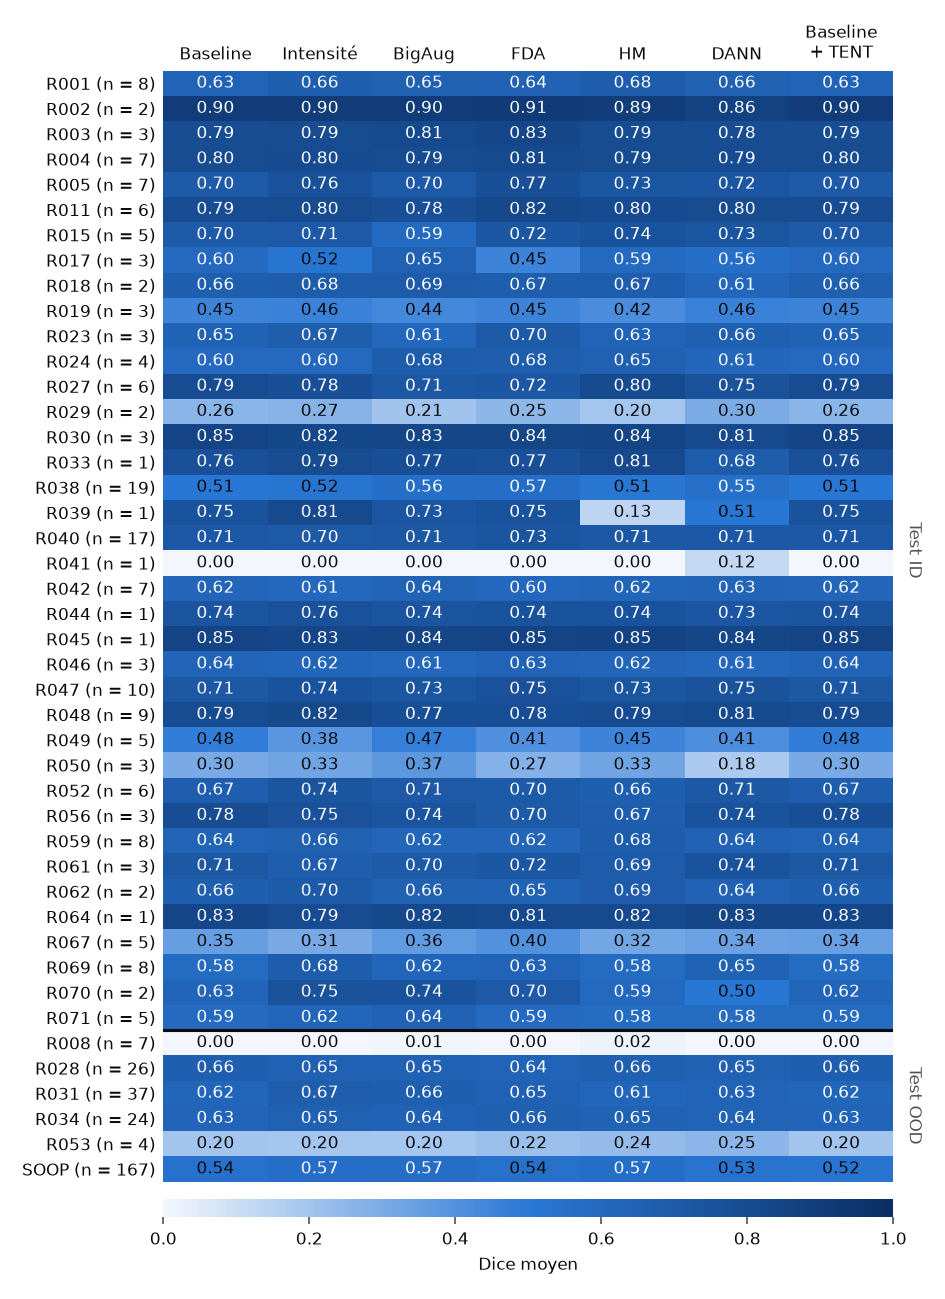
\includegraphics[width=\linewidth]{figures/rq3/rq3_dice_par_centre.png}
  \caption{Dice moyen par centre de test (ID et OOD) et par technique. HM : histogram matching.}
  \label{fig:rq3-dice-centre}
\end{figure}

\subsection{Taille des lésions}

La taille est le facteur le plus net.
Sur les 265 sujets OOD, la corrélation de Spearman entre le volume de la lésion et le Dice (modèle intensité) vaut $\rho = 0{,}53$ ($p < 10^{-4}$).
Le tableau~\ref{tab:rq3-taille} et la figure~\ref{fig:rq3-dice-taille} montrent que toutes les techniques suivent le même profil.
L'intensité gagne surtout entre 1 et 50~ml (0,50 et 0,67 contre 0,46 et 0,64 pour la baseline). BigAug gagne surtout au-dessus de 10~ml (0,68 et 0,77 contre 0,64 et 0,74).

\begin{table}[htbp]
  \centering
  \caption{Dice moyen par volume de lésion sur le test OOD (Dice ID entre parenthèses). L'adaptation continue porte sur un sous-ensemble des sujets.}
  \label{tab:rq3-taille}
  \small
  \begin{tabular}{lcccc}
    \toprule
    Technique & $< 1$~ml & 1--10~ml & 10--50~ml & $\geq 50$~ml \\
    \midrule
    Sujets OOD (ID) & 41 (34) & 86 (65) & 80 (48) & 58 (38) \\
    \midrule
    Baseline & 0,31 (0,48) & 0,46 (0,58) & 0,64 (0,71) & 0,74 (0,83) \\
    Intensité & 0,33 (0,46) & 0,50 (0,59) & 0,67 (0,74) & 0,74 (0,83) \\
    BigAug & 0,32 (0,43) & 0,48 (0,59) & 0,68 (0,75) & 0,77 (0,83) \\
    FDA & 0,30 (0,44) & 0,46 (0,61) & 0,66 (0,74) & 0,75 (0,84) \\
    Histogram matching & 0,33 (0,49) & 0,49 (0,58) & 0,66 (0,71) & 0,74 (0,83) \\
    DANN & 0,29 (0,46) & 0,45 (0,58) & 0,63 (0,73) & 0,75 (0,83) \\
    Baseline + TENT & 0,32 (0,48) & 0,46 (0,58) & 0,62 (0,71) & 0,71 (0,82) \\
    Continue (contrôlée) & 0,35 & 0,48 & 0,60 & 0,81 \\
    \bottomrule
  \end{tabular}
\end{table}

\begin{figure}[htbp]
  \centering
  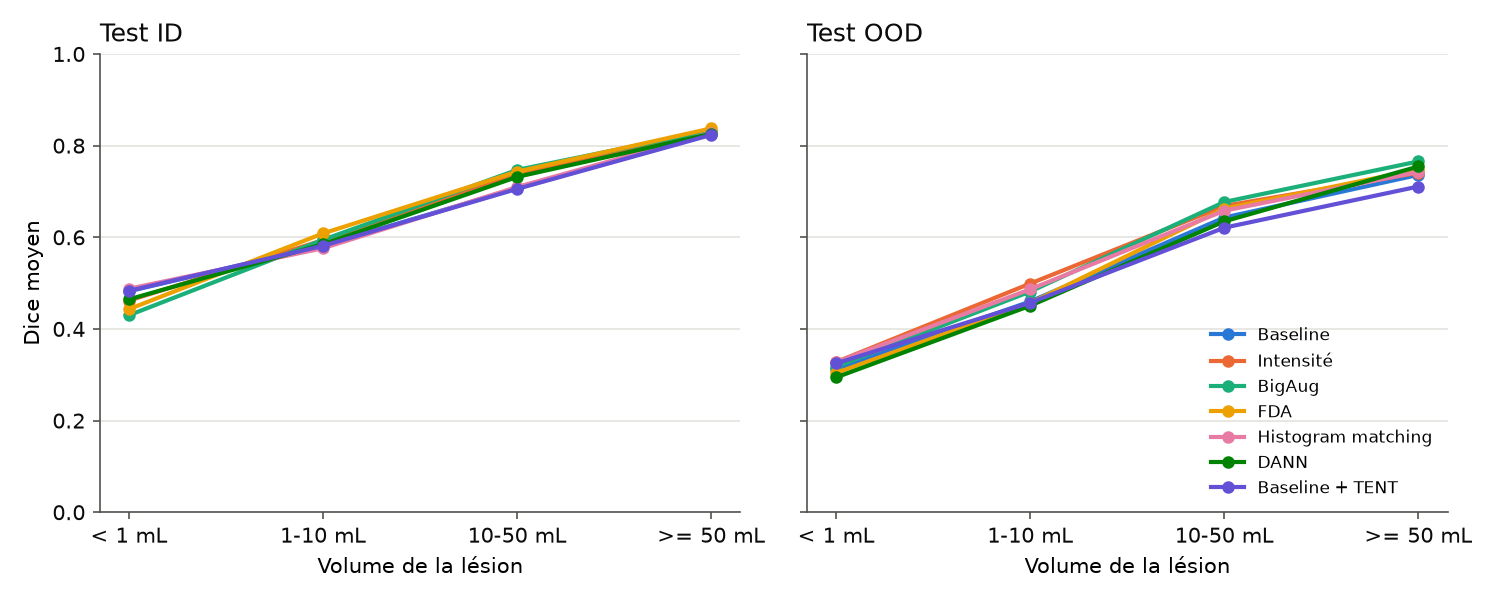
\includegraphics[width=\linewidth]{figures/rq3/rq3_dice_par_taille.png}
  \caption{Dice moyen par classe de volume de lésion, sur les tests ID (à gauche) et OOD (à droite).}
  \label{fig:rq3-dice-taille}
\end{figure}

La figure~\ref{fig:rq3-echecs-taille} reprend le test OOD en y ajoutant l'adaptation continue contrôlée.

\begin{figure}[htbp]
  \centering
  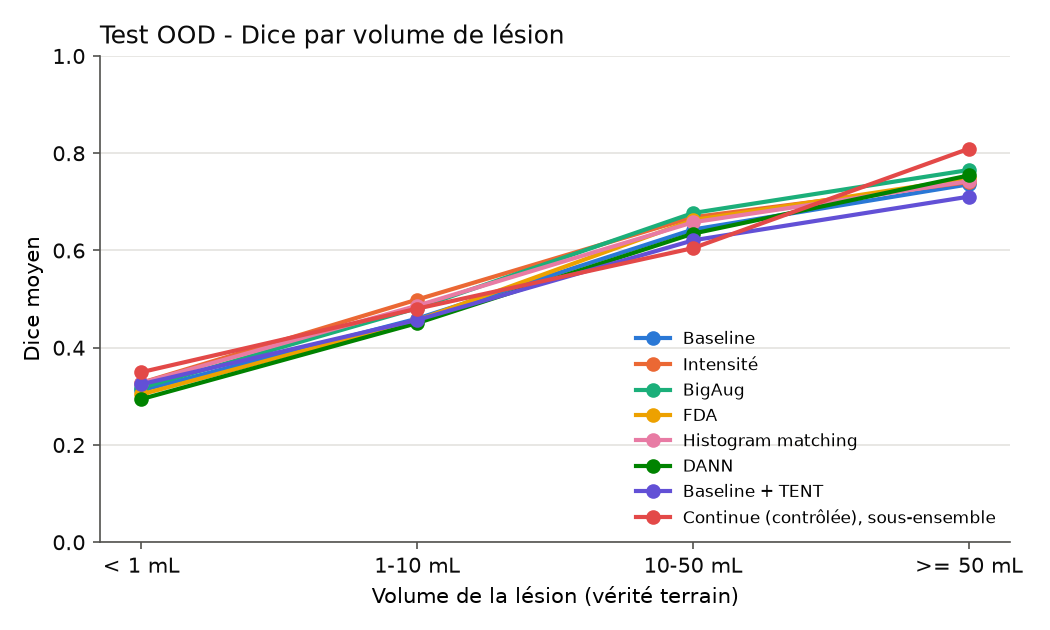
\includegraphics[width=0.8\linewidth]{figures/rq3/rq3_echecs_dice_par_taille.png}
  \caption{Dice moyen par volume de lésion sur le test OOD, avec l'adaptation continue contrôlée (sous-ensemble préquentiel).}
  \label{fig:rq3-echecs-taille}
\end{figure}

\subsection{Centre R008}

Toutes les techniques obtiennent un Dice nul ou presque sur R008. Le Dice moyen de BigAug est de 0,006 sur le centre ; un seul sujet est non nul, à 0,04 (tableau~\ref{tab:rq3-bigaug-intensite} ; moyenne arrondie à 0,01 dans le tableau~\ref{tab:rq3-centres}). Celui d'histogram matching est de 0,019, avec un seul sujet non nul, à 0,13 (tableau~\ref{tab:rq3-hm-intensite}). Le détail par sujet est dans \nolinkurl{zoom_R008_R053.csv}.
\begin{itemize}
  \item Six sujets sur sept sont imagés au premier jour après l'AVC. Leurs lésions font de 0,1 à 4,1~ml.
  \item Les lésions sont peu visibles en T1 : contraste médian de $-0{,}17$, contre $-0{,}50$ à $-0{,}98$ dans les autres centres OOD.
  \item Les intensités sont atypiques : 1,1 à 1,7~\% des voxels du cerveau dépassent $z = 3$, contre 0,003~\% en médiane chez les autres sujets OOD (\nolinkurl{contraste_lesions.csv}).
  \item Le modèle prédit de 0,4 à 33,6~ml répartis en nombreuses composantes, pour une différence du nombre de lésions de 9 à 67.
  \item À l'examen des coupes, vaisseaux, sinus et dure-mère apparaissent hyperintenses.
\end{itemize}
% Les coupes de R008 (figures/rq3/rq3_echecs_coupes_R008.png) ne sont pas incluses :
% ce sont des images ATLAS, non versionnées ; elles se régénèrent avec adaptation/analyse_echecs.py.

\emph{Hypothèse.} La séquence T1 de R008 aurait été acquise après injection de gadolinium, en phase aiguë.
La lésion n'y aurait pas encore le contraste T1 des lésions chroniques, majoritaires à l'entraînement.
Le décalage serait alors à la fois d'acquisition et de stade clinique.
Cette hypothèse reste à vérifier sur le protocole d'acquisition de R008 et sur l'écart entre la date de l'IRM et celle de l'annotation.

\subsection{Centre R053}

Le Dice moyen de R053 est de 0,20 sur quatre sujets ; un cinquième sujet a un masque vide et est exclu du Dice.
Deux lésions minuscules (0,13 et 0,015~ml) ont un Dice de 0. Les deux autres (1,5 et 2,6~ml) obtiennent 0,27 et 0,52.
Les intensités sont dans la norme (99\textsuperscript{e} centile du z-score proche de 1,8) et le contraste vaut $-0{,}50$.
L'échec s'explique par la taille des lésions, pas par un décalage d'intensité. Avec quatre sujets, la moyenne du centre est très instable.

\subsection{Distance de domaine}

La distance de Wasserstein entre histogrammes d'intensité (\nolinkurl{analysis/center_distance.py}, référence = tous les autres centres) ne prédit pas le Dice dans nos runs (\nolinkurl{spearman.csv}).
\begin{itemize}
  \item Sur les six centres OOD, $\rho$ va de $-0{,}43$ à $-0{,}03$ selon la technique ($p$ de 0,40 à 0,96). Avec la MMD, $\rho$ va de $-0{,}37$ à $-0{,}09$.
  \item Sur les 44 centres de test (ID et OOD), $\rho$ va de 0,03 à 0,12 ($p \geq 0{,}44$).
\end{itemize}
La figure~\ref{fig:rq3-distance} en donne deux contre-exemples. R053 est l'un des centres les plus proches (0,020) et l'un des pires. R031 est éloigné (0,164) et parmi les meilleurs.
Six centres offrent une puissance très faible : nous ne concluons pas à l'absence de lien, seulement qu'il n'apparaît pas ici.

\begin{figure}[htbp]
  \centering
  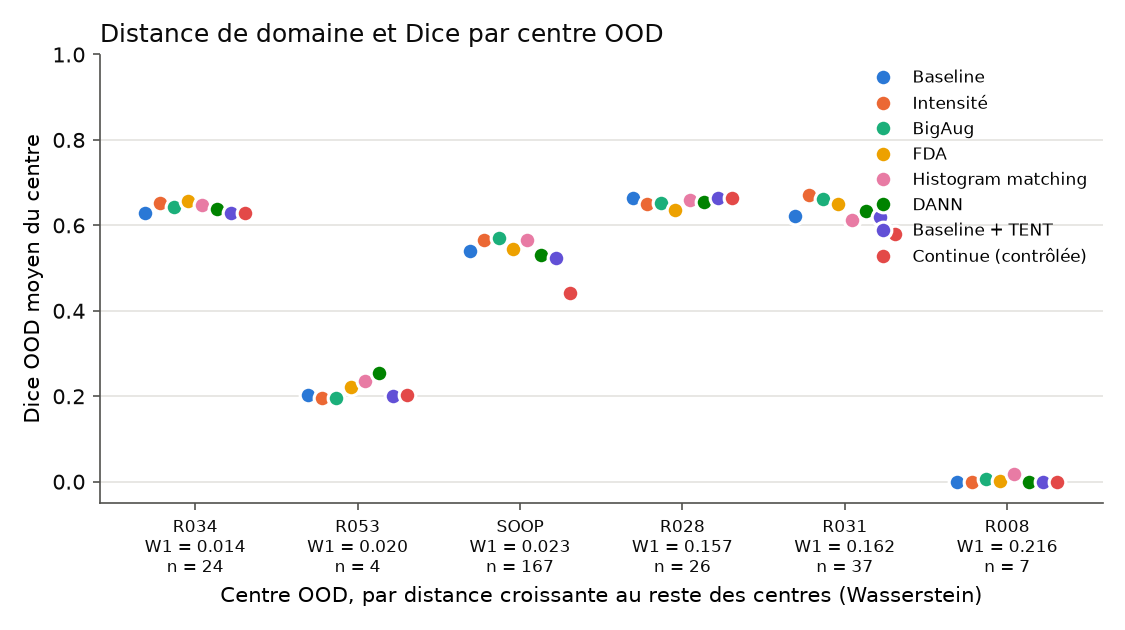
\includegraphics[width=0.8\linewidth]{figures/rq3/rq3_echecs_distance_dice.png}
  \caption{Dice OOD moyen par centre, les centres étant rangés par distance croissante au reste des centres.}
  \label{fig:rq3-distance}
\end{figure}

Au niveau des sujets, le contraste de la lésion n'est que faiblement lié au Dice ($\rho = -0{,}19$, $p = 0{,}001$). La figure~\ref{fig:rq3-contraste} montre ce nuage et place les sujets de R008 et R053.

\begin{figure}[htbp]
  \centering
  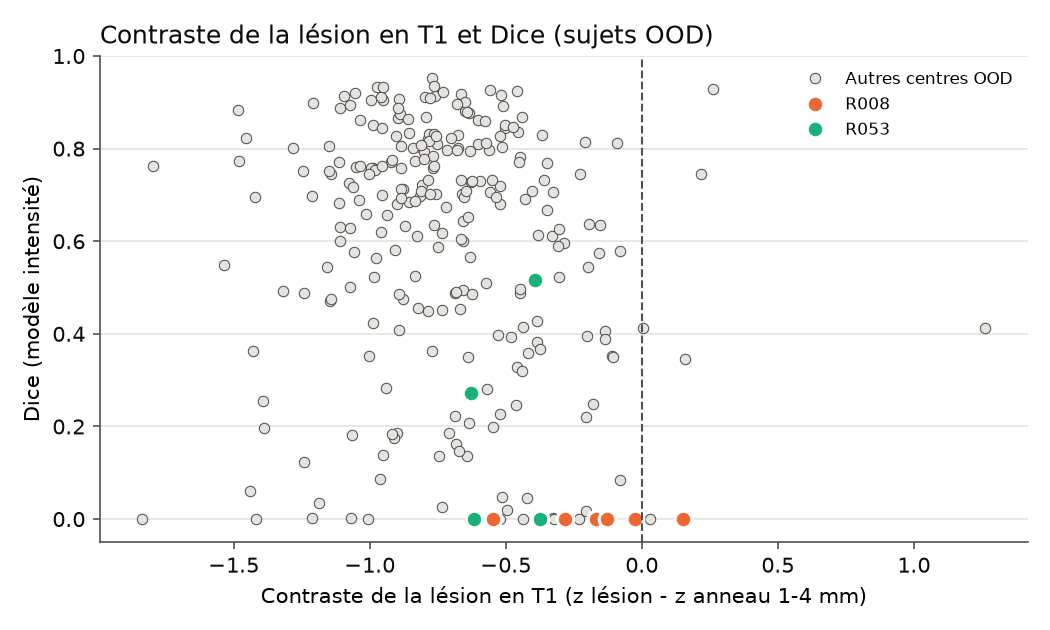
\includegraphics[width=0.8\linewidth]{figures/rq3/rq3_echecs_contraste_dice.png}
  \caption{Contraste T1 de la lésion et Dice (modèle intensité) pour les sujets OOD ; R008 et R053 sont mis en évidence.}
  \label{fig:rq3-contraste}
\end{figure}

\section{Adaptation continue contrôlée}
\label{sec:rq3-continue}

\paragraph{Protocole.}
L'expérience est réalisée par le script \nolinkurl{adaptation/continual.py}.
Ses sorties se trouvent dans le dossier \nolinkurl{adaptation/outputs/rq3/adaptation_continue/}.
Le modèle baseline reçoit les six centres OOD l'un après l'autre, par lots de quatre sujets : 28 lots, 108 sujets, au plus 24 par centre. Il n'est jamais réinitialisé.
L'évaluation est préquentielle : chaque lot est d'abord noté (Dice), puis utilisé pour l'adaptation, sans étiquettes.
Quatre stratégies sont comparées sur les mêmes lots :
\begin{itemize}
  \item \texttt{fige} : le modèle reste inchangé ;
  \item \texttt{auto\_apprentissage} : pseudo-étiquettes, tous les poids sont mis à jour ;
  \item \texttt{tent} : TENT appliqué en continu ;
  \item \texttt{controlee} : TENT dans un modèle candidat, promu seulement si trois conditions sont réunies. (1) La distance du lot dépasse un seuil calibré sur la source (0,077). (2) L'entropie baisse sur des patches neufs. (3) Le Dice sur un jeu de garde étiqueté de la source ne baisse pas de plus de 0,01. Cette stratégie rejoue aussi des exemples des centres déjà vus et des patches de la source.
\end{itemize}
L'oubli est mesuré après chaque centre, par le Dice sur 16 sujets fixes du test ID et sur les premiers sujets des centres OOD déjà vus.

\paragraph{Résultats.}
Le tableau~\ref{tab:rq3-continue} résume les quatre stratégies (\nolinkurl{resume.json}, \nolinkurl{oubli.csv}).

\begin{table}[htbp]
  \centering
  \caption{Adaptation continue sur les six centres OOD : Dice préquentiel et oubli.}
  \label{tab:rq3-continue}
  \small
  \begin{tabular}{lcccc}
    \toprule
    Stratégie & \makecell{Dice\\préquentiel} & \makecell{Dice ID\\(début $\rightarrow$ fin)} & Oubli ID & \makecell{Oubli OOD\\moyen} \\
    \midrule
    Figé & 0,528 & 0,635 $\rightarrow$ 0,635 & 0,000 & 0,000 \\
    Auto-apprentissage & 0,486 & 0,635 $\rightarrow$ 0,583 & 0,052 & 0,033 \\
    TENT continu & 0,526 & 0,635 $\rightarrow$ 0,632 & 0,002 & 0,000 \\
    Contrôlée & 0,527 & 0,635 $\rightarrow$ 0,634 & 0,001 & 0,000 \\
    \bottomrule
  \end{tabular}
\end{table}

Les décisions lot par lot sont dans \nolinkurl{decisions.csv}.
\begin{itemize}
  \item \textbf{Détection.} Un décalage est détecté sur 15 lots sur 28 : tous ceux de R008, R028 et R031, et un lot sur six de SOOP. Il n'est jamais détecté sur R034 ni R053, les centres les plus proches de la source.
  \item \textbf{Promotions.} Douze candidats sont promus : deux pour R008, six pour R028, trois pour R031 et un pour SOOP. Trois candidats de R031 sont refusés parce que leur entropie augmente.
  \item \textbf{Oubli.} La stratégie contrôlée évite l'oubli de l'auto-apprentissage (0,001 contre 0,052 sur le test ID).
  \item \textbf{Gain.} Elle n'améliore pas le Dice par rapport au modèle figé (0,527 contre 0,528).
\end{itemize}

\paragraph{Lecture du résultat.}
L'absence de gain s'explique par la nature des décalages détectés.
R028 et R031 sont déjà bien segmentés par le modèle figé (0,66 et 0,58 en préquentiel).
Sur R008, le problème tient au contraste des lésions (section~\ref{sec:rq3-echecs}), qu'une adaptation des normalisations ne peut pas créer.
Les Dice préquentiels portent sur 108 des 268 sujets OOD ; ils ne se comparent pas directement au tableau~\ref{tab:rq3-resultats}.

\section{Limites}
\label{sec:rq3-limites}

\begin{itemize}
  \item \textbf{Un seul pli et une seule graine.} Les IC traduisent la variabilité des sujets, pas celle de l'entraînement.
  \item \textbf{Reprise de DANN.} La run a été coupée à l'itération 35\,889 et reprise jusqu'à 40\,000. La reprise restaure les poids, l'optimiseur, le taux d'apprentissage, $\lambda$, la position de l'échantillonneur et les états aléatoires des processus de chargement. Le contrôle automatique a validé la première ligne reprise (itération 35\,900, taux $1{,}29 \times 10^{-4}$, $\lambda = 0{,}9771$). Seuls les masques de Dropout du classifieur de centre ne sont pas restaurés. Le meilleur modèle, à l'itération 24\,000, précède de toute façon la coupure.
  \item \textbf{Environnement de DANN.} DANN a été entraînée sur Colab avec torch 2.14.1+cu130 jusqu'à l'itération 35\,889, puis sur Kaggle avec torch 2.11.0+cu130, comme les autres runs. Les deux plateformes utilisent un GPU T4 et CUDA 13.0. Le meilleur modèle (itération 24\,000) vient de la partie Colab. La différence de version de torch peut changer les calculs numériques ; son effet n'a pas été mesuré.
  \item \textbf{Poids de DANN.} Avec un poids de 1, la première run DANN a divergé (perte totale de 10\,508 à l'itération 100 et de 33 millions à l'itération 400). Le poids de 0,1 et la LayerNorm ont été choisis pour la stabilité, sans recherche d'hyperparamètres. Un autre poids pourrait donner un autre résultat.
  \item \textbf{Validation sur des centres non vus.} Ses lésions sont plus petites que celles du test. Elle sert à choisir le checkpoint, mais son Dice (environ 0,43) n'estime pas la performance ID.
  \item \textbf{Diagnostic fp16.} La première baseline, entraînée en fp16, a produit des NaN : des patches entiers donnaient des logits NaN dès l'itération 160 à 180 environ, alors que le fp32 restait stable sur les mêmes lots. Toutes les runs ont été refaites en fp32, environ deux fois plus lentement. La couche qui déborde n'a pas été localisée.
  \item \textbf{Bug de reprise corrigé.} Dans la version du code utilisée pour les runs, la ligne de progression écrasait la file des états aléatoires sauvegardés pour la reprise. Le défaut ne concerne que les reprises, donc uniquement DANN. Il a été corrigé et couvert par un test. Le checkpoint de DANN a été réparé avant la reprise en ne gardant que les quatre derniers états, qui étaient les bons ; les poids n'ont pas changé.
  \item \textbf{Référence de la distance de domaine.} Pour chaque centre, la référence de \nolinkurl{center_distance} regroupe tous les autres centres, OOD compris, et pas seulement les centres d'entraînement du pli~0. La distance mesure donc l'écart au reste du jeu de données, pas exactement l'écart à ce que le modèle a vu.
  \item \textbf{Version du code d'histogram matching.} Cette run a utilisé une version ultérieure du code (\texttt{dbf2f28} au lieu de \texttt{7449c49}), qui ne diffère que par la correction du bug de reprise. Sans DANN ni reprise, les deux versions donnent des poids identiques (vérifié par un court entraînement sur CPU, pour la baseline et l'intensité).
  \item \textbf{Quota GPU.} Avec 30~h par semaine sur Kaggle, aucun autre pli n'a été entraîné, et l'histogram matching a été lancé après les autres techniques.
  \item \textbf{Portée de TENT et de l'adaptation continue.} Les deux ne sont évalués que sur la baseline.
\end{itemize}

\section{Conclusion}
\label{sec:rq3-conclusion}

Sur le pli~0, seule l'augmentation d'intensité améliore le Dice OOD de façon significative après correction : $+0{,}024$ [0,008 ; 0,041], $p$ Holm $= 0{,}0068$ (tableau~\ref{tab:rq3-resultats}).
BigAug atteint le même Dice OOD (0,577), mais son gain n'est pas significatif après correction ($p$ Holm $= 0{,}14$), et la comparaison directe ne sépare pas les deux techniques ($+0{,}001$ [$-0{,}010$ ; 0,012], tableau~\ref{tab:rq3-bigaug-intensite}).
Histogram matching n'est pas significatif non plus ($+0{,}017$, $p$ Holm $= 0{,}49$) ; il reste en dessous de l'intensité en Dice OOD ($-0{,}007$ [$-0{,}023$ ; 0,009]), avec un écart net sur R031 (tableau~\ref{tab:rq3-hm-intensite}).
Aucune technique ne supprime l'écart ID $-$ OOD, qui reste compris entre 0,075 et 0,104.
FDA, DANN et TENT n'améliorent pas le test OOD ; TENT le dégrade légèrement.
L'adaptation continue contrôlée évite l'oubli sans améliorer le Dice (tableau~\ref{tab:rq3-continue}).
L'analyse des échecs montre que les cas les plus difficiles tiennent aux lésions elles-mêmes, petites ou peu contrastées en T1, plutôt qu'à la distance d'intensité entre centres.
Le livrable C8 (\nolinkurl{adaptation/inference.py}) segmente un T1 et renvoie le masque et le volume de la lésion.
Le modèle retenu pour la démonstration est celui de l'intensité.
À Dice égal avec BigAug, ce choix repose d'abord sur son gain significatif après correction, ensuite sur un entraînement plus court (5,0~h contre 8,1~h).
Son F1 des lésions est supérieur à celui de BigAug (0,450 contre 0,420) mais inférieur à celui de la baseline (0,477) : ce n'est qu'un argument relatif face à BigAug.
Histogram matching a le plus faible écart absolu de volume (9,1~ml contre 10,0~ml pour l'intensité) et un F1 des lésions supérieur à celui de la baseline (0,486 contre 0,477).
Il n'a pas été retenu, car son gain en Dice n'est pas significatif et il exigerait d'harmoniser aussi chaque volume à l'inférence, avec l'histogramme de référence de R059.
Ces constats orientent la suite vers la prédiction des cas à risque, en particulier les lésions de moins de 1~ml et les AVC en phase aiguë.


\chapter*{Conclusion générale}
\addcontentsline{toc}{chapter}{Conclusion générale}
\label{chap:conclusion}

Le projet fournit une chaîne complète, de l'inventaire des données à une démonstration qui segmente une IRM T1 et en mesure la lésion.
Le chapitre~\ref{chap:yosra} établit les données, les partitions communes et les mesures du décalage entre centres.
Le chapitre~\ref{chap:anas} montre qu'un nnU-Net 3D dépasse nettement le CNN 2.5D, qu'un réseau plus grand n'apporte rien à budget de temps égal, et que les modèles restent sous-entraînés.
Le chapitre~\ref{chap:rq3} montre que, sur son protocole, seule l'augmentation d'intensité améliore le Dice OOD de façon significative après correction, sans supprimer l'écart entre ID et OOD, et que la distance d'intensité entre centres ne prédit pas le Dice OOD.
Dans les chapitres~\ref{chap:anas} et~\ref{chap:rq3}, les cas les plus difficiles sont les petites lésions et les AVC aigus, peu visibles en T1.
Deux limites demeurent : aucun Transformer n'a été évalué, si bien que la question RQ2 n'est traitée que par la comparaison d'un CNN 2.5D, d'un U-Net 3D et d'un ResEnc U-Net ; et les deux protocoles d'évaluation restent distincts.
La suite naturelle est d'évaluer les meilleurs modèles sur un même découpage et sur plusieurs plis.

\appendix
% Annexe glossaire, à inclure dans docs/rapport/rapport.tex après \appendix.
% Traduction du glossaire du rapport nnU-Net 3D d'Anas (partie « Terms »).

\chapter{Glossaire}
\label{chap:glossaire}

\begin{table}[htbp]
  \centering
  \caption{Termes utilisés dans le rapport.}
  \label{tab:glossaire}
  \small
  \begin{tabular}{lp{0.62\linewidth}}
    \toprule
    Terme & Signification \\
    \midrule
    Dice & recouvrement entre la lésion prédite et celle de l'expert : $2 \times$ recouvrement / (prédit + vrai). 0 = aucun, 1 = parfait \\
    HD95 & distance entre les bords de la lésion prédite et de la vraie lésion, en mm, en ignorant les 5~\% de points les plus éloignés ; plus bas est meilleur \\
    F1 par lésion & compte des lésions au lieu de voxels : une lésion est trouvée si la prédiction la touche ; combine lésions trouvées et fausses alarmes \\
    ID / OOD & in-distribution (centres vus à l'entraînement) / out-of-distribution (centres jamais vus) \\
    Pseudo-Dice & Dice que nnU-Net calcule sur des patches de validation pendant l'entraînement ; plus élevé que le vrai Dice sur des IRM entières, il sert seulement à suivre l'entraînement \\
    Époque & ici, 250 lots de 2 patches \\
    Sous-apprentissage & le modèle n'a pas encore assez appris : les erreurs d'entraînement et de validation baissent toutes deux encore \\
    Sur-apprentissage & le modèle mémorise le jeu d'entraînement : l'erreur d'entraînement baisse pendant que l'erreur de validation remonte \\
    Supervision profonde & la perte est aussi calculée sur les sorties de plus basse résolution du décodeur, ce qui aide les couches profondes à apprendre \\
    Normalisation d'instance & remet chaque carte de caractéristiques de chaque IRM à une moyenne de 0 et un écart-type de 1 ; fonctionne avec des lots de seulement 2 \\
    Leaky ReLU & activation : $x$ si $x > 0$, sinon $0{,}01\,x$ \\
    Bloc résiduel & deux convolutions plus un raccourci qui ajoute l'entrée à la sortie, si bien que l'information et les gradients peuvent sauter le bloc \\
    Augmentation au test & prédire l'IRM et ses copies en miroir, puis faire la moyenne \\
    \bottomrule
  \end{tabular}
\end{table}


\bibliographystyle{plain}
\bibliography{docs/rapport/references_rq3}

\end{document}
